This section describes the data files for a \mf Groundwater Flow (GWF) Model.  A GWF Model is added to the simulation by including a GWF entry in the MODELS block of the simulation name file.

There are three types of spatial discretization approaches that can be used with the GWF Model.  Input for a GWF Model may be entered in a structured form, like for previous MODFLOW versions, in that users specify cells using their layer, row, and column indices.  Users may also work with a layered grid in which cells are defined using vertices.  In this case, users specify cells using the layer number and the cell number.  Lastly, GWF Models may be entered as fully unstructured models, in which cells are specified using only their cell number.  Once a spatial discretization approach has been selected, then all input with cell indices must be entered accordingly.

The GWF Model is designed to permit input to be gathered, as it is needed, from many different files.  Likewise, results from the model calculations can be written to a number of output files. The GWF Model Listing File is a key file to which the GWF model output is written.  As \mf runs, information about the GWF Model is written to the GWF Model Listing File, including much of the input data (as a record of the simulation) and calculated results.  Details about the files used by each package are provided in this section on the GWF Model Instructions.

\mf is further designed to allow the user to control the amount, type, and frequency of information to be output. Much of the output will be written to the Simulation and GWF Model Listing Files, but some model output can be written to other files.  The Listing Files can become very large for common models.  Text editors are useful for examining the Listing File. The GWF Model Listing File includes a summary of the input data read for all packages.  In addition, the GWF Model Listing File optionally contains calculated head controlled by time step, and the overall volumetric budget controlled by time step. The Listing Files also contain information about solver convergence and error messages.  Output to other files can include head and cell-by-cell flow terms for use in calculations external to the model or in user-supplied applications such as plotting programs.

The GWF Model reads a file called the Name File, which specifies most of the files that will be used in a simulation. Several files are always required whereas other files are optional depending on the simulation. The Output Control Package receives instructions from the user to control the amount and frequency of output.  Details about the Name File and the Output Control Package are described in this section.

\subsection{Information for Existing MODFLOW Users}
\mf contains most of the functionality of MODFLOW-2005, MODFLOW-NWT, MODFLOW-USG, and MODFLOW-LGR.  To the existing MODFLOW user, however, \mf will feel different from previous MODFLOW versions.  Some packages have been divided, renamed, or removed, and some capabilities, which previously caused confusion or were implemented due to computer memory limitations, are no longer supported (for example, ``quasi-3d confining units'' are not supported in the GWF Model).  The form of the input files for \mf is different from previous MODFLOW versions in that input files are now divided into blocks, and keywords are used to specify options and input variables.  Extensive testing was used as part of the development process to ensure that \mf simulation results are identical to the results from previous MODFLOW versions.  In some cases, it was not possible to exactly replicate the simulation results from previous MODFLOW versions.  In those cases, the differences could be explained by an option that is no longer supported, or because of slight differences in the underlying formulation.  

The following list, which is repeated from \cite{modflow6gwf}, summarizes the major differences between the GWF Model in \mf and previous versions of MODFLOW.  This list is intended for those with a general understanding of the capabilities in previous versions of MODFLOW.

\begin{enumerate}

\item The GWF Model in \mf supports three alternative input packages for specifying the grid used to discretize the groundwater system.  
\begin{itemize}
\item The Discretization (DIS) Package defines a grid based on layers, rows, and columns.  In this report, this type of grid is referred to as a ``regular MODFLOW grid'' because it corresponds to traditional MODFLOW grids.  An interior cell in a regular MODFLOW grid is connected to four adjacent cells in the same layer, to one overlying cell, and to one underlying cell.
\item The Discretization by Vertices (DISV) Package defines a grid using a list of ($x$, $y$) vertex pairs and the number of layers.  A list of vertices is provided by the user to define a two-dimensional horizontal grid in plan view.  This list of vertices may define a regular MODFLOW grid, or they may define more complex grids, such as grids consisting of triangles, hexagons, or Voronoi polygons, for example.  This same two-dimensional horizontal grid applies to each layer in the model.  Cells defined using the DISV Package are referenced by layer number and by the cell number within the horizontal grid.  Within a layer, a cell may be horizontally connected to any number of surrounding cells in that layer.  In the vertical direction a cell can be connected to only one overlying cell and only one underlying cell.  Grids defined with the DISV Package are considered to be unstructured.
\item The unstructured Discretization (DISU) Package is the most flexible of the three packages and is patterned after the unstructured grid implemented in MODFLOW-USG.  For each cell, the user specifies a list of connected cells and the connection properties.  When the DISU Package is used, cells are referenced only by their cell number; unlike the MODFLOW-USG approach, there is no concept of a layer in the DISU Package in \mfcomma but cells may still overlie or underlie one another.  
\end{itemize}

\item For the layered grid types supported in the GWF Model (DIS and DISV), cells can be permanently excluded from the grid for the simulation.  Input values (such as hydraulic conductivity) are still required for these excluded cells, and the program will write special codes or zero values for output, but the program does not allocate memory or store values for excluded cells during run time.  In this case, the matrix equations are formulated for a reduced system in which only the included cells are numbered.  Users can also mark excluded cells as ``vertical pass-through cells.''  When these vertical pass-through cells are encountered, the program connects the cells overlying and underlying the pass-through cell.  This capability allows ``pinched'' cells to be removed from the solution.  These options to exclude cells or exclude them as pass-through cells are available for the DIS and DISV Packages through specification of the IDOMAIN array; the IDOMAIN capability is not available for the DISU Package.

\item There is no longer a Basic Package input file.  Initial head values are specified using an Initial Conditions (IC) Package, and constant heads are specified using the Time Varying Specified Head (CHD) Package.  Cells that are permanently excluded from the simulation can be eliminated using the IDOMAIN capability entered through the DIS or DISV Packages.  For a cell that may transition from inactive (``dry'') to active (``wet'') during a simulation, the user can start the cell as inactive by assigning an initial head below the cell bottom.

\item The Newton-Raphson formulations and accompanying upstream weighting schemes implemented in MODFLOW-NWT and MODFLOW-USG for handling dry or nearly dry cells have been synthesized into a single formulation.  The Newton-Raphson formulation in the GWF Model for \mf remains an optional alternative to the standard formulation used in most previous MODFLOW versions. Much of this report is focused on systematically explaining standard and Newton-Raphson formulations for the GWF Model and its packages.

\item Information on temporal discretization, such as number of stress periods, period lengths, number of time steps, and time step multipliers, is specified at the simulation level, rather than for an individual model.  This information is provided in the Timing Module, which controls the temporal discretization and applies to all models within a simulation.  The Timing Module is part of the \mf framework and is described separately in \cite{modflow6framework}.

\item Aquifer properties used to calculate hydraulic conductance are specified in the Node Property Flow (NPF) Package.  In \mfcomma the NPF Package calculates intercell conductance values, manages cell wetting and drying, and adds Newton-Raphson terms for intercell flow expressions.  The NPF Package allows individual cells to be designated as confined or convertible; this was not an option in previous MODFLOW versions as the designation was by layer.  The NPF Package also has several options for simulating drainage problems and problems involving perched aquifers where an active cell overlies a partially saturated cell.  The default NPF Package behavior (in which none of these options are set) is the most stable for typical groundwater problems.  The default NPF Package behavior does not correspond to the default behavior for other MODFLOW internal flow packages.  The NPF Package does not support quasi-3D confining units.  The NPF Package replaces the Layer Property Flow (LPF), Block-Centered Flow (BCF), and Upstream Weighting (UPW) Packages from previous MODFLOW versions.  Capabilities of the Hydrogeologic Unit Flow (HUF) Package \citep{anderman2000modflow, anderman2003modflow} are not supported in the GWF Model of \mf.

\item Aquifer storage properties are specified in the Storage (STO) Package.  If the STO Package is excluded for a model, then the model represents steady-state conditions.  If the STO Package is included, users can specify steady-state or transient conditions by stress period as needed.  Compressible storage contributions are no longer approximated as zero for unconfined layers; contributions from pore drainage and compressible storage are separated in the model output.

\item The Horizontal Flow Barrier (HFB) Package \citep{hsieh1993hfb, modflow2005} in \mf allows barrier properties and locations to change by stress period.  The capability to change barriers by stress period was not supported in previous MODFLOW versions.

\item The GWF Model in \mf allows multiple stress packages of the same type to be specified for a single GWF Model.  This capability is also available in MODFLOW-CDSS \citep{banta2011modflow}.  Package entries written to the budget file and budget terms in the listing file are written separately for each package.

\item Input of boundary conditions for simulation in multiple stress periods is entered differently than for previous MODFLOW versions. Boundary conditions are specified for a stress period in a ``PERIOD'' block. These boundary conditions remain active at their specified values until a subsequent ``PERIOD'' block is encountered or the end of the simulation is reached.  Individual entries within the ``PERIOD'' block can be specified as a time-series entry.  Values for these variables, which may correspond to a well pumping rate or a drain conductance, for example, are interpolated from a time-series dataset, for each time step, using several different interpolation options.

\item The Flow and Head Boundary (FHB) Package \citep{leake1997documentation, modflow2005} is not supported in \mf; however, its capabilities can be replicated using the WEL Package, the CHD Package, and the new time-series capability.

\item There is one Evapotranspiration (EVT) Package for \mf. The \mf EVT Package contains the functionality of the MODFLOW-2005 EVT Package, the Segmented Evapotranspiration (ETS) Package \citep{modflowdrtpack}, and the Riparian Evapotranspiration (RIP-ET) Package \citep{modflowripetpack}.

\item A new Multi-Aquifer Well (MAW) Package replaces the Multi-Node Well (MNW1 and MNW2) Packages \citep{halford2002, konikow2009}. The new package does not contain all of the options available in MNW1 and MNW2, but it does contain the most commonly used ones.  It also has new capabilities for simulating flowing wells. The MAW Package is solved as part of the matrix solution and is tightly coupled with the GWF Model. This tight coupling with the GWF Model may substantially improve convergence for simulations of groundwater flow to multi-aquifer wells.

\item Most capabilities of the Stream (STR) and Streamflow Routing (SFR) Packages \citep{prudic1989str, modflowsfr1pack, modflowsfr2pack} are included in \mf as a new SFR Package.  The new SFR Package contains all of the functionality of the SFR Package in MODFLOW-2005 with the following exceptions: (a) the concept of a ``segment'' has been eliminated, (b) only rectangular cross sections are supported for stream reaches, and (c) unsaturated zone flow beneath stream reaches cannot be simulated.

\item A new Lake (LAK) Package replaces the existing MODFLOW Lake Packages \citep{modflowlak3pack}. In addition to being able to represent lakes that are incised into the model grid, the new LAK Package can also represent sub-grid scale lakes that are conceptualized as being on top of the model.  The status of a lake can change during the simulation between \texttt{ACTIVE}, \texttt{INACTIVE}, and \texttt{CONSTANT}.  The new package contains most of the capabilities available in previous LAK Packages, including the ability to apply recharge and evapotranspiration to underlying cells if the lake is dry.  The LAK Package documented here does not represent unsaturated zone flow beneath a lake or support for the coalescing lake option described in \cite{modflowlak3pack}. 

\item A new Unsaturated Zone Flow (UZF) Package, based on the one described by \cite{UZF}, is included in the GWF Model of \mfdot The new UZF Package allows the UZF capabilities to be applied to only selected cells of the GWF model. The new UZF Package also supports a multi-layer option, which allows for vertical heterogeneity in unsaturated zone properties.

\item A new Water Mover (MVR) Package is included in \mfdot  The MVR Package can be used to transfer water from individual ``provider'' features of selected packages (WEL, DRN, RIV, GHB, MAW, SFR, LAK, and UZF) to individual ''receiver'' features of the advanced packages (MAW, SFR, LAK, and UZF).  Simple rules are used to determine how much of the available water is moved from the provider to the receiver, which allows management controls to be represented. 

\item \mf contains a flexible new Observation (OBS) capability, which allows the user to define many different types of continuous-in-time or point-in-time observations.  The new OBS capability replaces the Observation Process \citep{hill2000modflow}, the Gage Package, and the HYDMOD capability \citep{hanson1999documentation} in previous MODFLOW versions.  Flow, head, and drawdown observations can be obtained for the GWF Model.  Flow and other package-specific observations, such as the head in a multi-aquifer well or lake stage, for example, can also be obtained.  These observed values can be used subsequently with a parameter estimation program or they can be used to make time-series plots of a wide range of simulated values.  The new OBS capability does not support specification of field-measured observations, calculation of residuals, or interpolation within a grid, as was supported in previous versions of the MODFLOW OBS Process.

\item The GWF Model described in this report does not support the following list of packages and capabilities.  Support for some of these capabilities may be added in future \mf versions.
  \begin{itemize}
    \item Drain with Return Flow Package \citep{modflowdrtpack}
    \item Reservoir Package \citep{fenske1996documentation},
    \item Seawater Intrusion Package \citep{bakker2013documentation},
    \item Surface-Water Routing Process \citep{hughes2012documentation},
    \item Connected Linear Network Process \citep{modflowusg},
    \item Parameter Value File \citep{modflow2005}, and
    \item Link to the MT3DMS Contaminant Transport Model \citep{zheng2001modflow}.  However, MT3D-USGS can read the head and budget files created by MODFLOW 6, but only if the GWF Model uses the DIS Package.  MT3D-USGS will not work with GWF output if the DISV or DISU Packages are used.
  \end{itemize}

\end{enumerate}

In addition to this list of major differences, there are other differences between \mf and previous MODFLOW versions in terms of the input and output files and the way users interact with the program.  These differences include:

\begin{enumerate}

\item The \mf program begins by reading a simulation name file.  The simulation name file must be named ``mfsim.nam.''

\item All real variables in \mf are declared as double precision floating point numbers.  Real variables written to binary output files are also written in double precision.

\item Unit numbers are no longer specified by the user.  Unit numbers are determined automatically by \mf based upon user-provided file names.

\item The GWF Model name file contains a list of packages that are active for the model.  Names for output files are not specified in the name file.  Names for output files, such as the head and budget files are specified in the OC Package.

\item The EXTERNAL option for reading arrays and lists is no longer supported; however, the OPEN/CLOSE option is still supported.  The SFAC option for lists is no longer supported; however, many packages allow for specification of an auxiliary variable which can serve as a multiplier on a column of values in the list.

\item The CHD Package contains new flexibility.  Cells can transition between constant-head cells and active cells during the simulation.  This was not allowed in previous MODFLOW versions.  Also, the CHD Packages no longer performs linear interpolation between a starting (shead) and ending head (ehead).  Only a single head value is provided for each constant-head cell.  The capability to linearly interpolate a head value for each time step within a stress period is available through the use of time series.

\item There are two different forms of input for the RCH and EVT Packages: array-based input and list-based input.  For models that use DIS Package, the RCH and EVT input can be provided as arrays, which is consistent with previous MODFLOW versions.  To use array input, the user must specify the READASARRAYS keyword in the options block.  The READASARRAYS option can also be used for models that use the DISV Package.  If the READASARRAYS option is not specified, then input to the RCH and EVT Packages is provided in list form.  List-based input is the only option supported when the DISU Package is used.

List-based input offers several advantages over the array-based input for specifying recharge and evapotranspiration.  First, multiple list entries can be specified for a single cell.  This makes it possible to divide a cell into multiple areas, and assign a different recharge or evapotranspiration rate for each area (perhaps based on land use or some other criteria).  In this case, the user would likely specify an auxiliary variable to serve as a multiplier.  This multiplier would be calculated by the user and provided in the input file as the fractional cell are for the individual recharge entries.  Another advantage to using list-based input for specifying recharge is that ``boundnames'' can be specified.  Boundnames work with the Observations capability and can be used to sum recharge or evapotranspiration rates for entries with the same boundname.  A disadvantage of the list-based input is that one cannot easily assign recharge or evapotranspiration rates to the entire model without specifying a list of model cells.  For this reason \mf also supports array-based input.

\item Calculation and reporting of drawdown for the model grid is no longer supported, as this calculation is easily performed as a postprocessing step.  Calculation of drawdown is supported as an observation type by the OBS Package; 
drawdown is calculated as the difference between the starting head specified in the IC Package and the calculated head.

\item There are differences in the output files created by \mfcomma such as:
\begin{itemize}

\item A separate listing file is written for the simulation.  This simulation listing file contains information about the simulation, including solver information.  Separate listing files are written for each GWF Model that is part of the simulation.

\item Unformatted head files written by \mf are consistent with those written by previous MODFLOW versions; however, all real values are written in double precision.

\item The budget file written by the GWF Model is always written in ``compact'' form (as opposed to full three-dimensional arrays) and uses new method codes, which allow model and package names to be written to the file.  Simulated intercell flows are always written in a compressed sparse row format, even for regular MODFLOW grids.

\item Information about the GWF Model grid is written to a separate file, called a ``binary grid file'' each time the model runs.  The binary grid file can be used by postprocessing programs for subsequent analysis.  The format of the binary grid file is described in a section on ``Binary Output Files.''

\end{itemize}


\end{enumerate}


\subsection{Array Input (READARRAY)}
Some GWF Model packages require arrays of information to be provided by the user.  This information is read using a generic READARRAY capability in \mfdot  Within this user guide, variables that are read with READARRAY are marked accordingly, as shown in example input instructions for a DATA block.  

\begin{lstlisting}[style=blockdefinition]
BEGIN DATA
  ARRAY1
    <array1(nval)> -- READARRAY
END DATA
\end{lstlisting}

\noindent In this example, the uppercase ARRAY1 is a text string that is recognized by the program.  While reading through the DATA block, the program would recognize ARRAY1, and would then use READARRAY to fill \texttt{array1} with \texttt{nval} values.

\subsubsection{READARRAY Control Line}

READARRAY works similar to the array readers in previous MODFLOW versions.  It begins by reading a control line.  The control line has one of three forms shown below, and is limited to a length of 999 characters.

\begin{lstlisting}[style=blockdefinition]
1. CONSTANT <constant> 
\end{lstlisting}
With CONSTANT, all values in the array are set equal to \texttt{constant}. 

\begin{lstlisting}[style=blockdefinition]
2. INTERNAL [FACTOR <factor>] [IPRN <iprn>] 
\end{lstlisting}
With INTERNAL, the individual array elements will be read from the same file that contains the control line. 

\begin{lstlisting}[style=blockdefinition]
3. OPEN/CLOSE <fname> [FACTOR <factor>] [(BINARY)] [IPRN <iprn>]
\end{lstlisting}
With OPEN/CLOSE, the array will be read from the file whose name is specified by \texttt{fname}. This file will be opened just prior to reading the array and closed immediately after the array is read. A file that is read using this control line can contain only a single array. 

\subsubsection{READARRAY Variable Descriptions}

\begin{description}

\item \texttt{<constant>}---is a real number constant for real arrays and an integer constant for integer arrays. The \texttt{constant} value is assigned to the entire array. 

\item \texttt{FACTOR <factor>}---are a keyword and a real number factor for real arrays and an integer factor for integer arrays. The individual elements of the array are multiplied by \texttt{factor} after they are read. If \texttt{factor} is specified as 0, then it is changed to 1.

\item \texttt{(BINARY)}---is an option that indicates the OPEN/CLOSE file contains array data in binary (unformatted) form. A binary file that can be read by MODFLOW may be created in only two ways. The first way is to use MODFLOW to create the file by saving heads in a binary file. This is commonly done when the user desires to use computed heads from one simulation as initial heads for a subsequent simulation. The other way to create a binary file is to write a special program that generates a binary file.  ``(BINARY)'' can be specified only when the control line is OPEN/CLOSE.

\item \texttt{IPRN <iprn>}---are a keyword and a flag that indicates whether the array being read should be written to the Listing File after the array has been read and a code for indicating the format that should be used when the array is written. The format codes are the same as for MODFLOW-2005. IPRN is set to zero when the specified value exceeds those defined. If IPRN is less than zero or if the keyword and flag are omitted, the array will not be printed.

\end{description}

\begin{longtable}{p{2cm} p{2cm} p{2cm} p{2cm}}
\caption{IPRN Code and corresponding print formats for array readers.  These print codes determine how the user-provided array is written to the list file} 
\tabularnewline
\hline
\hline
\textbf{IPRN} & \textbf{Real} & \textbf{Integer} \\
\hline
\endhead
\hline
\endfoot
0 & 10G11.4 & 10I11 \\
1 & 11G10.3 & 60I1 \\
2 & 9G13.6 & 40I2 \\
3 & 15F7.1 & 30I3 \\
4 & 15F7.2 & 25I4 \\
5 & 15F7.3 & 20I5 \\
6 & 15F7.4 & 10I11 \\
7 & 20F5.0 & 25I2 \\
8 & 20F5.1 & 15I4 \\
9 & 20F5.2 & 10I6 \\
10 & 20F5.3 &  \\
11 & 20F5.4 &  \\
12 & 10G11.4 & \\
13 & 10F6.0 &  \\
14 & 10F6.1 &  \\
15 & 10F6.2 &  \\
16 & 10F6.3 &  \\
17 & 10F6.4 &  \\
18 & 10F6.5 &  \\
19 & 5G12.5 &  \\
20 & 6G11.4 &  \\
21 & 7G9.2 &  \\
%\label{table:ndim}
\end{longtable}


\subsubsection{READARRAY Examples}

The following examples use free-format control lines for reading an array. The example array is a real array consisting of 4 rows with 7 columns per row: 

\begin{lstlisting}[style=inputfile]
CONSTANT 5.7      This sets an entire array to the value "5.7". 
INTERNAL FACTOR 1.0 IPRN 3            This reads the array values from the 
 1.2 3.7 9.3 4.2 2.2 9.9 1.0      file that contains the control line. 
 3.3 4.9 7.3 7.5 8.2 8.7 6.6      Thus, the values immediately follow the 
 4.5 5.7 2.2 1.1 1.7 6.7 6.9      control line. 
 7.4 3.5 7.8 8.5 7.4 6.8 8.8 
OPEN/CLOSE inp.txt FACTOR 1.0 IPRN 3    Read array from formatted file "inp.dat". 
OPEN/CLOSE inp.bin FACTOR 1.0 (BINARY) IPRN 3     Read array from binary file "inp.bin". 
OPEN/CLOSE test.dat FACTOR 1.0 IPRN 3     Read array from file "test.dat". 
\end{lstlisting}


Some arrays define information that is required for the entire model grid, or part of a model grid.  This type of information is provided in a special type of data block called a ``GRIDDATA'' block.  For example, hydraulic conductivity is required for every cell in the model grid.  Hydraulic conductivity is read from a ``GRIDDATA'' block in the NPF Package input file.  For GRIDDATA arrays with one value for every cell in the model grid, the arrays can optionally be read in a LAYERED format, in which an array is provided for each layer of the grid.  Alternatively, the array can be read for the entire model grid.  As an example, consider the GRIDDATA block for the IC Package shown below:

\lstinputlisting[style=blockdefinition]{./mf6ivar/tex/gwf-ic-griddata.dat}

Here, the initial heads for the model are provided in the \texttt{strt} array.  If the optional LAYERED keyword is present, then a separate array is provided for each layer.  If the LAYERED keyword is not present, then the entire starting head array is read at once.  The LAYERED keyword may be useful to discretization packages of type DIS and DISV, which support the concept of layers.  Models defined with the DISU Package are not layered.

For a structured DIS model, the READARRAY utility is used to read arrays that are dimensioned to the full size of the grid (of size \texttt{nlay*nrow*ncol}). This utility first reads an array name, which associates the input to be read with the desired array.  For these arrays, an optional keyword ``LAYERED'' can be located next to the array name.  If ``LAYERED'' is detected, then a control line is provided for each layer and the array is filled with values for each model layer.  If the ``LAYERED'' keyword is absent, then a single control line is used and the entire array is filled at once.

For example, the following block shows one way the starting head array (STRT) could be specified for a model with 4 layers.  Following the array name and the ``LAYERED'' keyword are four control lines, one for each layer.

\begin{lstlisting}[style=inputfile]
  STRT LAYERED
     CONSTANT 10.0  #layer 1
     CONSTANT 10.0  #layer 2
     CONSTANT 10.0  #layer 3
     CONSTANT 10.0  #layer 4
\end{lstlisting}

In this next example, the ``LAYERED'' keyword is absent.  In this case, the control line applies to the entire \texttt{strt} array.  One control line is required, and a constant value of 10.0 will be assigned to STRT for all cells in the model grid.

\begin{lstlisting}[style=inputfile]
  STRT
     CONSTANT 10.0  #applies to all cells in the grid
\end{lstlisting}

\subsection{List Input}
Some items consist of several variables, such as layer, row, column, stage, and conductance, for example.  List input refers to a block of data with a separate item on each line.  For some common list types, the first set of variables is a cell identifier (denoted as \texttt{cellid} in this guide), such as layer, row, and column. With lists, the input data for each item must start on a new line. All variables for an item are assumed to be contained in a single line.  Each input variable has a data type, which can be Double Precision, Integer, or Character. Integers are whole numbers and must not include a decimal point or exponent. Double Precision numbers can include a decimal point and an exponent. If no decimal point is included in the entered value, then the decimal point is assumed to be at the right side of the value. Any printable character is allowed for character variables. 

Variables starting with the letters I-N are most commonly integers; however, in some instances, a character string may start with the letters I-N. Variables starting with the letters A-H and O-Z are primarily double precision numbers; however, these variable names may also be used for character data.  In \mf all variables are explicitly declared within the source code, as opposed to the implicit type declaration in previous MODFLOW versions.  This explicit declaration means that the variable type can be easily determined from the source code.

Free formatting is used throughout the input instructions.  With free format, values are not required to occupy a fixed number of columns in a line. Each value can occupy one or more columns as required to represent the value; however, the values must still be included in the prescribed order. One or more spaces, or a single comma optionally combined with spaces, must separate adjacent values. Also, a numeric value of zero must be explicitly represented with 0 and not by one or more spaces when free format is used, because detecting the difference between a space that represents 0 and a space that represents a value separator is not possible. Free format is similar to Fortran's list directed input.

Two capabilities included in Fortran's list-directed input are not included in the free-format input implemented in \mfdot Null values in which input values are left unchanged from their previous values are not allowed. In general, MODFLOW's input values are not defined prior to their input.  A ``/'' cannot be used to terminate an input line without including values for all the variables; data values for all required input variables must be explicitly specified on an input line.  For character data, MODFLOW's free format implementation is less stringent than the list-directed input of Fortran. Fortran requires character data to be delineated by apostrophes. MODFLOW does not require apostrophes unless a blank or a comma is part of a character variable.

As an example of a list, consider the PERIOD block for the GHB Package.  The input format is  shown below:

\lstinputlisting[style=blockdefinition]{./mf6ivar/tex/gwf-ghb-period.dat}

Each line represents a separate item, which consists of variables.  In this case, the first variable of the item, \texttt{cellid} is an array of size \texttt{ncelldim}.  The next two variables of the item are \texttt{bhead} and \texttt{cond}.  Lastly, the item has two optional variables, \texttt{aux} and \texttt{boundname}.  Three of the variables shown in the list are colored in blue.  Variables that are colored in blue mean that they can be represented with a time series.  The time series capability is described in the section on Time-Variable Input in this document.  

The following is simple example of a PERIOD block for the GHB Package, which shows how a list is entered by the user.

\begin{lstlisting}[style=inputfile]
BEGIN PERIOD 1
#      lay       row       col     stage      cond
         1        13         1     988.0     0.038
         1        14         9    1045.0     0.038
END PERIOD
\end{lstlisting}

As described earlier in the section on ``Block and Keyword Input,'' block information can be read from a separate text file.  To activate reading a list from separate text file, the first and only entry in the block must be a control line of the following form:  

\begin{lstlisting}[style=blockdefinition]
  OPEN/CLOSE <fname>
\end{lstlisting}

\noindent where \texttt{fname} is the name of the file containing the list.  Lists for the stress packages (CHD, WEL, DRN, RIV, GHB, RCH, and EVT) have an additional BINARY option.  The BINARY  option is not supported for the advanced stress packages (LAK, MAW, SFR, UZF).  The BINARY options is specified as follows:

\begin{lstlisting}[style=blockdefinition]
  OPEN/CLOSE <fname> [(BINARY)]
\end{lstlisting}

If the (BINARY) keyword is found on the control line, then the file is opened as an unformatted file on unit 99, and the list is read.  There are a number of requirements for using the (BINARY) option for lists.  All stress package lists begin with integer values for the \texttt{cellid} (layer, row, and column, for example).  These values must be represented as integer numbers in the unformatted file.  Also, all auxiliary data must be included in the binary file; auxiliary data must be represented as double precision numbers.  Lastly, the (BINARY) option does not support entry of \texttt{boundname}, and so the BOUNDNAMES option should not be activated in the OPTIONS block for the package.  

\subsection{Units of Length and Time}
The GWF Model formulates the groundwater flow equation without using prescribed length and time units. Any consistent units of length and time can be used when specifying the input data for a simulation. This capability gives a certain amount of freedom to the user, but care must be exercised to avoid mixing units.  The program cannot detect the use of inconsistent units.  For example, if hydraulic conductivity is entered in units of feet per day and pumpage as cubic meters per second, the program will run, but the results will be meaningless. Other processes generally are expected to work with consistent length and time units; however, other processes could conceivably place restrictions on which units are supported.

The user can set flags that specify the length and time units (see the input instructions for the Timing Module and Spatial Discretization Files), which may be useful in various parts of MODFLOW.  For example, the program will label the table of simulation time with time units if the time units are specified by the optional TIME\_UNITS label, which can be set in the TDIS Package.  If the time units are not specified, the program still runs, but the table of simulation time does not indicate the time units. An optional LENGTH\_UNITS label can be set in the Discretization Package. Situations in other processes may require that the length or time units be specified.  In such situations, the input instructions will state the requirements. Remember that specifying the unit flags does not enforce consistent use of units.  The user must insure that consistent units are used in all input data.

\subsection{Steady-State Simulations}
A steady-state simulation is represented by a single stress period having a single time step with the storage term set to zero. Setting the number and length of stress periods and time steps is the responsibility of the Timing Module of the \mf framework. The length of the stress period and time step will not affect the head solution because the time derivative is not calculated in a steady-state problem. Setting the storage term to zero is the responsibility of the Storage Package. Most other packages need not "know" that a simulation is steady state.

A GWF Model also can be mixed transient and steady state because each stress period can be designated transient or steady state.  Thus, a GWF Model can start with a steady-state stress period and continue with one or more transient stress periods.  The settings for controlling steady-state and transient options are in the Storage Package.  If the Storage Package is not specified for a GWF Model, then the storage terms are zero and the GWF Model will be steady state.

\subsection{Volumetric Budget}
A summary of all inflows (sources) and outflows (sinks) of water is called a water budget.  The water budget for the GWF Model is termed a volumetric budget because volumes of water and volumetric flow rates are involved; thus strictly speaking, a volumetric budget is not a mass balance, although this term has been used in other model reports.  \mf calculates a water budget for the overall model as a check on the acceptability of the solution, and to provide a summary of the sources and sinks of water to the flow system.  The water budget is printed to the GWF Model Listing File for selected time steps.

Numerical solution techniques for simultaneous equations do not always result in a correct answer; in particular, iterative solvers may stop iterating before a sufficiently close approximation to the solution is attained.  A water budget provides an indication of the overall acceptability of the solution.  The system of equations solved by the model actually consists of a flow continuity statement for each model cell.  Continuity should also exist for the total flows into and out of the model---that is, the difference between total inflow and total outflow should equal the total change in storage.  In the model program, the water budget is calculated independently of the equation solution process, and in this sense may provide independent evidence of a valid solution.

The total budget as printed in the output does not include internal flows between model cells---only flows into or out of the model as a whole. For example, flow to or from rivers, flow to or from constant-head cells, and flow to or from wells are all included in the overall budget terms.  Flow into and out of storage is also considered part of the overall budget inasmuch as accumulation in storage effectively removes water from the flow system and storage release effectively adds water to the flow---even though neither process, in itself, involves the transfer of water into or out of the ground-water regime.  Each hydrologic package calculates its own contribution to the budget.

For every time step, the budget subroutine of each hydrologic package calculates the rate of flow into and out of the system due to the process simulated by the package.  The inflows and outflows for each component of flow are stored separately.  Most packages deal with only one such component of flow.  In addition to flow, the volumes of water entering and leaving the model during the time step are calculated as the product of flow rate and time-step length.  Cumulative volumes, from the beginning of the simulation, are then calculated and stored.

The GWF Model uses the inflows, outflows, and cumulative volumes to write the budget to the Listing File at the times requested by the model user.  When a budget is written, the flow rates for the last time step and cumulative volumes from the beginning of simulation are written for each component of flow.  Inflows are written separately from outflows.  Following the convention indicated above, water entering storage is treated as an outflow (that is, as a loss of water from the flow system) while water released from storage is treated as an inflow (that is, a source of water to the flow system).  In addition, total inflow and total outflow are written, as well as the difference between total inflow and outflow.  The difference is then written as a percentage error, calculated using the formula:

\begin{equation}
D = \frac{100 (IN-OUT)}{(IN + OUT) / 2}
\end{equation}

\noindent where $D$ is the percentage error term, $IN$ is the total inflow to the system, and $OUT$ is the total outflow.

If the model equations are solved correctly, the percentage error should be small.  In general, flow rates may be taken as an indication of solution validity for the time step to which they apply, while cumulative volumes are an indication of validity for the entire simulation up to the time of the output.  The budget is written to the GWF Model Listing File at the end of each stress period whether requested or not.

\subsection{Cell-By-Cell Flows}
In some situations, calculating flow terms for various subregions of the model is useful.  To facilitate such calculations, provision has been made to save flow terms for individual cells in a separate binary file so they can be used in computations external to the model itself.  These individual cell flows are referred to here as ``cell-by-cell'' flow terms and are of four general types: (1) cell-by-cell stress flows, or flows into or from an individual cell caused by one of the external stresses represented in the model, such as evapotranspiration or recharge; (2) cell-by-cell storage terms, which give the rate of accumulation or depletion of storage in an individual cell; and (3) internal cell-by-cell flows, which are actually the flows across individual cell faces---that is, between adjacent model cells.  These four kinds of cell-by-cell flow terms are discussed further in subsequent paragraphs.  To save any of these cell-by-cell terms, two flags in the model input must be set.  The input to the Output Control file indicates the time steps for which cell-by-cell terms are to be saved. In addition, each hydrologic package includes an option called SAVE\_FLOWS that must be set if the cell-by-cell terms computed by that package are to be saved.  Thus, if the appropriate option in the Evapotranspiration Package input is set, cell-by-cell evapotranspiration terms will be saved for each time step for which the saving of cell-by-cell flow is requested through the Output Control Option.  Only flow values are saved in the cell-by-cell files; neither water volumes nor cumulative water volumes are included.  The flow dimensions are volume per unit time, where volume and time are in the same units used for all model input data.  The cell-by-cell flow values are stored in unformatted form to make the most efficient use of disk space; see the Budget File section toward the end of this user guide for information on how the data are written to a file.

The cell-by-cell storage term gives the net flow to or from storage in a variable-head cell.  The net storage for each cell in the grid is saved in transient simulations if the appropriate flags are set.  Withdrawal from storage in the cell is considered positive, whereas accumulation in storage is considered negative.

The cell-by-cell constant-head flow term gives the flow into or out of an individual constant-head cell (specified with the CHD Package).  This term is always associated with the constant-head cell itself, rather than with the surrounding cells that contribute or receive the flow.  A constant-head cell may be surrounded by as many as six adjacent variable-head cells for a regular grid or any number of cells for the other grid types.  The cell-by-cell calculation provides a single flow value for each constant-head cell, representing the algebraic sum of the flows between that cell and all of the adjacent variable-head cells.  A positive value indicates that the net flow is away from the constant-head cell (into the variable-head part of the grid); a negative value indicates that the net flow is into the constant-head cell.

The internal cell-by-cell flow values represent flows across the individual faces of a model cell.  Flows between cells are written in the compressed row storage format, whereby the flow between cell $n$ and each one of its connecting $m$ neighbor cells are contained in a single one-dimensional array.  Flows are positive for the cell in question.  Thus the flow reported for cell $n$ and its connection with cell $m$ is opposite in sign to the flow reported for cell $m$ and its connection with cell $n$.  These internal cell-by-cell flow values are useful in calculations of the groundwater flow into various subregions of the model, or in constructing flow vectors.

Cell-by-cell stress flows are flow rates into or out of the model, at a particular cell, owing to one particular external stress.  For example, the cell-by-cell evapotranspiration term for cell $n$ would give the flow out of the model by evapotranspiration from cell $n$.  Cell-by-cell stress flows are considered positive if flow is into the cell, and negative if out of the cell.

\newpage
\subsection{GWF Model Name File}
The GWT Model Name File specifies the options and packages that are active for a GWT model.  The Name File contains two blocks: OPTIONS  and PACKAGES. The length of each line must be 299 characters or less. The lines in each block can be in any order.  Files listed in the PACKAGES block must exist when the program starts. 

Comment lines are indicated when the first character in a line is one of the valid comment characters.  Commented lines can be located anywhere in the file. Any text characters can follow the comment character. Comment lines have no effect on the simulation; their purpose is to allow users to provide documentation about a particular simulation. 

\vspace{5mm}
\subsubsection{Structure of Blocks}
\lstinputlisting[style=blockdefinition]{./mf6ivar/tex/gwt-nam-options.dat}
\lstinputlisting[style=blockdefinition]{./mf6ivar/tex/gwt-nam-packages.dat}

\vspace{5mm}
\subsubsection{Explanation of Variables}
\begin{description}
% DO NOT MODIFY THIS FILE DIRECTLY.  IT IS CREATED BY mf6ivar.py 

\item \textbf{Block: OPTIONS}

\begin{description}
\item \texttt{list}---is name of the listing file to create for this GWT model.  If not specified, then the name of the list file will be the basename of the GWT model name file and the '.lst' extension.  For example, if the GWT name file is called ``my.model.nam'' then the list file will be called ``my.model.lst''.

\item \texttt{PRINT\_INPUT}---keyword to indicate that the list of all model stress package information will be written to the listing file immediately after it is read.

\item \texttt{PRINT\_FLOWS}---keyword to indicate that the list of all model package flow rates will be printed to the listing file for every stress period time step in which ``BUDGET PRINT'' is specified in Output Control.  If there is no Output Control option and ``PRINT\_FLOWS'' is specified, then flow rates are printed for the last time step of each stress period.

\item \texttt{SAVE\_FLOWS}---keyword to indicate that all model package flow terms will be written to the file specified with ``BUDGET FILEOUT'' in Output Control.

\end{description}
\item \textbf{Block: PACKAGES}

\begin{description}
\item \texttt{ftype}---is the file type, which must be one of the following character values shown in table~\ref{table:ftype}. Ftype may be entered in any combination of uppercase and lowercase.

\item \texttt{fname}---is the name of the file containing the package input.  The path to the file should be included if the file is not located in the folder where the program was run.

\item \texttt{pname}---is the user-defined name for the package. PNAME is restricted to 16 characters.  No spaces are allowed in PNAME.  PNAME character values are read and stored by the program for stress packages only.  These names may be useful for labeling purposes when multiple stress packages of the same type are located within a single GWT Model.  If PNAME is specified for a stress package, then PNAME will be used in the flow budget table in the listing file; it will also be used for the text entry in the cell-by-cell budget file.  PNAME is case insensitive and is stored in all upper case letters.

\end{description}


\end{description}

\begin{table}[H]
\caption{Ftype values described in this report.  The \texttt{Pname} column indicates whether or not a package name can be provided in the name file.  The capability to provide a package name also indicates that the GWT Model can have more than one package of that Ftype}
\small
\begin{center}
\begin{tabular*}{\columnwidth}{l l l}
\hline
\hline
Ftype & Input File Description & \texttt{Pname}\\
\hline
DIS6 & Rectilinear Discretization Input File \\
DISV6 & Discretization by Vertices Input File \\
DISU6 & Unstructured Discretization Input File \\
FMI6 & Flow Model Interface Package &  \\ 
IC6 & Initial Conditions Package \\
OC6 & Output Control Option \\
ADV6 & Advection Package \\ 
DSP6 & Dispersion Package \\ 
SSM6 & Source and Sink Mixing Package \\ 
MST6 & Mobile Storage and Transfer Package \\
IST6 & Immobile Storage and Transfer Package & * \\
CNC6 & Constant Concentration Package & * \\ 
SRC6 & Mass Source Loading Package & * \\ 
LKT6 & Lake Transport Package & * \\ 
SFT6 & Streamflow Transport Package & * \\ 
MWT6 & Multi-Aquifer Well Transport Package & * \\ 
UZT6 & Unsaturated Zone Transport Package & * \\ 
MVT6 & Mover Transport Package \\ 
OBS6 & Observations Option \\
\hline 
\end{tabular*}
\label{table:ftype}
\end{center}
\normalsize
\end{table}

\vspace{5mm}
\subsubsection{Example Input File}
\lstinputlisting[style=inputfile]{./mf6ivar/examples/gwt-nam-example.dat}



\newpage
\subsection{Structured Discretization (DIS) Input File}
Discretization information for structured grids is read from the file that is specified by ``DIS6'' as the file type.  Only one discretization input file (DISU6, DISV6 or DIS6) can be specified for a model.

\vspace{5mm}
\subsubsection{Structure of Blocks}
\lstinputlisting[style=blockdefinition]{./mf6ivar/tex/gwf-dis-options.dat}
\lstinputlisting[style=blockdefinition]{./mf6ivar/tex/gwf-dis-dimensions.dat}
\lstinputlisting[style=blockdefinition]{./mf6ivar/tex/gwf-dis-griddata.dat}

\vspace{5mm}
\subsubsection{Explanation of Variables}
\begin{description}
% DO NOT MODIFY THIS FILE DIRECTLY.  IT IS CREATED BY mf6ivar.py 

\item \textbf{Block: OPTIONS}

\begin{description}
\item \texttt{length\_units}---is the length units used for this model.  Values can be ``FEET'', ``METERS'', or ``CENTIMETERS''.  If not specified, the default is ``UNKNOWN''.

\item \texttt{NOGRB}---keyword to deactivate writing of the binary grid file.

\item \texttt{xorigin}---x-position of the lower-left corner of the model grid.  A default value of zero is assigned if not specified.  The value for XORIGIN does not affect the model simulation, but it is written to the binary grid file so that postprocessors can locate the grid in space.

\item \texttt{yorigin}---y-position of the lower-left corner of the model grid.  If not specified, then a default value equal to zero is used.  The value for YORIGIN does not affect the model simulation, but it is written to the binary grid file so that postprocessors can locate the grid in space.

\item \texttt{angrot}---counter-clockwise rotation angle (in degrees) of the lower-left corner of the model grid.  If not specified, then a default value of 0.0 is assigned.  The value for ANGROT does not affect the model simulation, but it is written to the binary grid file so that postprocessors can locate the grid in space.

\end{description}
\item \textbf{Block: DIMENSIONS}

\begin{description}
\item \texttt{nlay}---is the number of layers in the model grid.

\item \texttt{nrow}---is the number of rows in the model grid.

\item \texttt{ncol}---is the number of columns in the model grid.

\end{description}
\item \textbf{Block: GRIDDATA}

\begin{description}
\item \texttt{delr}---is the is the column spacing in the row direction.

\item \texttt{delc}---is the is the row spacing in the column direction.

\item \texttt{top}---is the top elevation for each cell in the top model layer.

\item \texttt{botm}---is the bottom elevation for each cell.

\item \texttt{idomain}---is an optional array that characterizes the existence status of a cell.  If the IDOMAIN array is not specified, then all model cells exist within the solution.  If the IDOMAIN value for a cell is 0, the cell does not exist in the simulation.  Input and output values will be read and written for the cell, but internal to the program, the cell is excluded from the solution.  If the IDOMAIN value for a cell is 1, the cell exists in the simulation.  If the IDOMAIN value for a cell is -1, the cell does not exist in the simulation.  Furthermore, the first existing cell above will be connected to the first existing cell below.  This type of cell is referred to as a ``vertical pass through'' cell.

\end{description}


\end{description}

\vspace{5mm}
\subsubsection{Example Input File}
\lstinputlisting[style=inputfile]{./mf6ivar/examples/gwf-dis-example.dat}


\newpage
\subsection{Discretization by Vertices (DISV) Input File}
Discretization information for DISV grids is read from the file that is specified by ``DISV6'' as the file type.  Only one discretization input file (DISV6, DISU6 or DIS6) can be specified for a model.

The approach for numbering cell and cell vertices for the DISV Package is shown in figure~\ref{fig:gwf-fig3-2}.  The list of vertices for a cell must be in clockwise order.  Closing of the cell polygon by repeating the first vertex as the last vertex is not required in the present implementation.  Internally within the program, however, the first vertex number is added to the end of the vertex list in order to close the polygon.  Thus, users have the option for whether or not to close cell polygons.

\begin{figure}[ht]
	\centering
	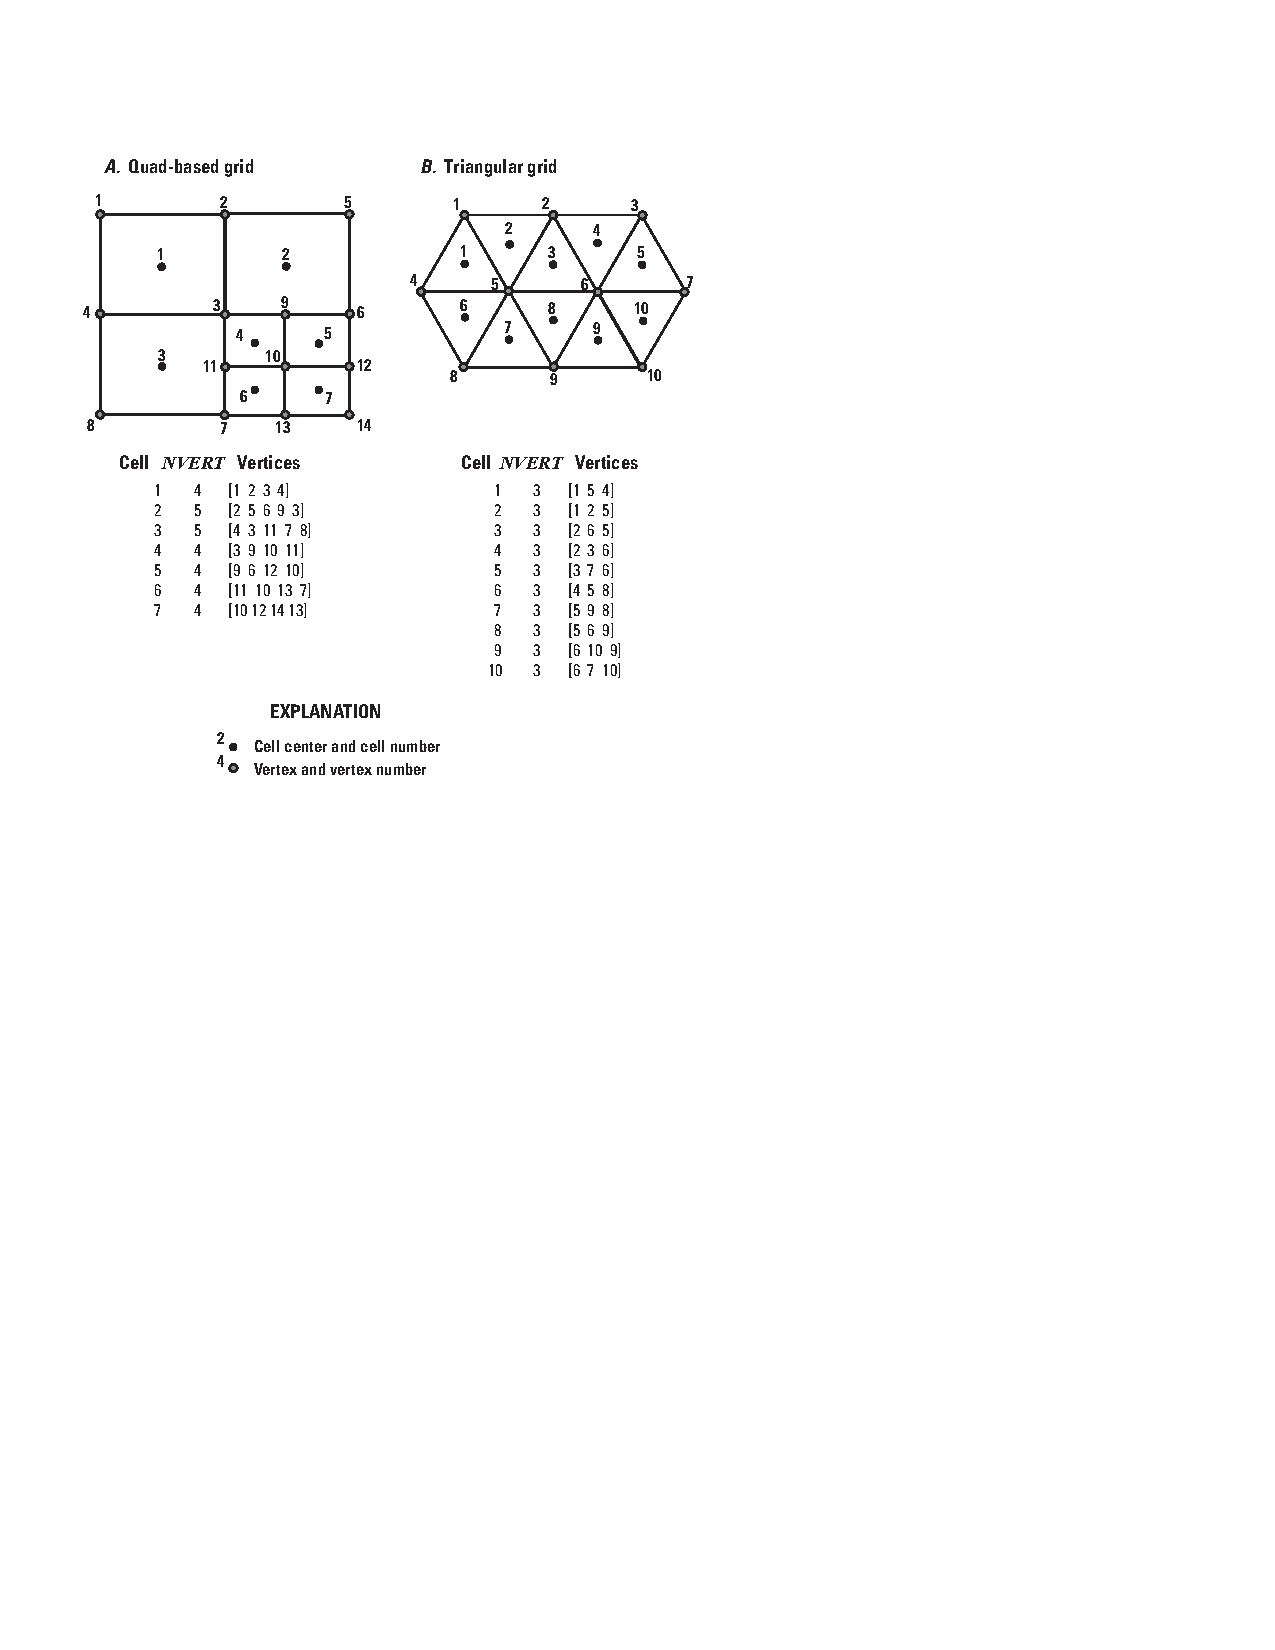
\includegraphics[scale=1.0]{gwf-fig3-2}
	\caption{Schematic diagram showing the vertices and cells defined using the Discretization by Vertices Package. The list of vertices used to define each cell must be in clockwise order.  From \cite{modflow6gwf}}
	\label{fig:gwf-fig3-2}
\end{figure}


\vspace{5mm}
\subsubsection{Structure of Blocks}
\lstinputlisting[style=blockdefinition]{./mf6ivar/tex/gwf-disv-options.dat}
\lstinputlisting[style=blockdefinition]{./mf6ivar/tex/gwf-disv-dimensions.dat}
\lstinputlisting[style=blockdefinition]{./mf6ivar/tex/gwf-disv-griddata.dat}
\lstinputlisting[style=blockdefinition]{./mf6ivar/tex/gwf-disv-vertices.dat}
\lstinputlisting[style=blockdefinition]{./mf6ivar/tex/gwf-disv-cell2d.dat}

\vspace{5mm}
\subsubsection{Explanation of Variables}
\begin{description}
% DO NOT MODIFY THIS FILE DIRECTLY.  IT IS CREATED BY mf6ivar.py 

\item \textbf{Block: OPTIONS}

\begin{description}
\item \texttt{length\_units}---is the length units used for this model.  Values can be ``FEET'', ``METERS'', or ``CENTIMETERS''.  If not specified, the default is ``UNKNOWN''.

\item \texttt{NOGRB}---keyword to deactivate writing of the binary grid file.

\item \texttt{xorigin}---x-position of the origin used for model grid vertices.  This value should be provided in a real-world coordinate system.  A default value of zero is assigned if not specified.  The value for \texttt{xorigin} does not affect the model simulation, but it is written to the binary grid file so that postprocessors can locate the grid in space.

\item \texttt{yorigin}---y-position of the origin used for model grid vertices.  This value should be provided in a real-world coordinate system.  If not specified, then a default value equal to zero is used.  The value for \texttt{yorigin} does not affect the model simulation, but it is written to the binary grid file so that postprocessors can locate the grid in space.

\item \texttt{angrot}---counter-clockwise rotation angle (in degrees) of the model grid coordinate system relative to a real-world coordinate system.  If not specified, then a default value of 0.0 is assigned.  The value for \texttt{angrot} does not affect the model simulation, but it is written to the binary grid file so that postprocessors can locate the grid in space.

\end{description}
\item \textbf{Block: DIMENSIONS}

\begin{description}
\item \texttt{nlay}---is the number of layers in the model grid.

\item \texttt{ncpl}---is the number of cells per layer.  This is a constant value for the grid and it applies to all layers.

\item \texttt{nvert}---is the total number of (x, y) vertex pairs used to characterize the horizontal configuration of the model grid.

\end{description}
\item \textbf{Block: GRIDDATA}

\begin{description}
\item \texttt{top}---is the top elevation for each cell in the top model layer.

\item \texttt{botm}---is the bottom elevation for each cell.

\item \texttt{idomain}---is an optional array that characterizes the existence status of a cell.  If the \texttt{idomain} array is not specified, then all model cells exist within the solution.  If the \texttt{idomain} value for a cell is 0, the cell does not exist in the simulation.  Input and output values will be read and written for the cell, but internal to the program, the cell is excluded from the solution.  If the \texttt{idomain} value for a cell is 1, the cell exists in the simulation.  If the \texttt{idomain} value for a cell is -1, the cell does not exist in the simulation.  Furthermore, the first existing cell above will be connected to the first existing cell below.  This type of cell is referred to as a ``vertical pass through'' cell.

\end{description}
\item \textbf{Block: VERTICES}

\begin{description}
\item \texttt{iv}---is the vertex number.  Records in the VERTICES block must be listed in consecutive order from 1 to \texttt{nvert}.

\item \texttt{xv}---is the x-coordinate for the vertex.

\item \texttt{yv}---is the y-coordinate for the vertex.

\end{description}
\item \textbf{Block: CELL2D}

\begin{description}
\item \texttt{icell2d}---is the cell2d number.  Records in the CELL2D block must be listed in consecutive order from 1 to \texttt{ncpl}.

\item \texttt{xc}---is the x-coordinate for the cell center.

\item \texttt{yc}---is the y-coordinate for the cell center.

\item \texttt{ncvert}---is the number of vertices required to define the cell.  There may be a different number of vertices for each cell.

\item \texttt{icvert}---is an array of integer values containing vertex numbers (in the VERTICES block) used to define the cell.  Vertices must be listed in clockwise order.  Cells that are connected must share vertices.

\end{description}


\end{description}

\vspace{5mm}
\subsubsection{Example Input File}
\lstinputlisting[style=inputfile]{./mf6ivar/examples/gwf-disv-example.dat}


\newpage
\subsection{Unstructured Discretization (DISU) Input File}
Discretization information for unstructured grids is read from the file that is specified by ``DISU6'' as the file type.  Only one discretization input file (DISU6, DISV6 or DIS6) can be specified for a model.

The shape and position of each cell can be defined using vertices.  This information is optional and is only read if the number of vertices (NVERT) in the DIMENSIONS block is specified and is assigned a value larger than zero.  If the vertices and two-dimensional cell information is provided in this file, then this information is also written to the binary grid file.  Providing this information may be useful for other postprocessing programs that read the binary grid file.

The DISU Package does not support the concept of layers, which is different from the DISU implementation in MODFLOW-USG.  In \mf~all grid input and output for models that use the DISU Package is entered or written as a one-dimensional array of size nodes.

\vspace{5mm}
\subsubsection{Structure of Blocks}
\lstinputlisting[style=blockdefinition]{./mf6ivar/tex/gwf-disu-options.dat}
\lstinputlisting[style=blockdefinition]{./mf6ivar/tex/gwf-disu-dimensions.dat}
\lstinputlisting[style=blockdefinition]{./mf6ivar/tex/gwf-disu-griddata.dat}
\lstinputlisting[style=blockdefinition]{./mf6ivar/tex/gwf-disu-connectiondata.dat}
\lstinputlisting[style=blockdefinition]{./mf6ivar/tex/gwf-disu-vertices.dat}
\lstinputlisting[style=blockdefinition]{./mf6ivar/tex/gwf-disu-cell2d.dat}

\vspace{5mm}
\subsubsection{Explanation of Variables}
\begin{description}
% DO NOT MODIFY THIS FILE DIRECTLY.  IT IS CREATED BY mf6ivar.py 

\item \textbf{Block: OPTIONS}

\begin{description}
\item \texttt{length\_units}---is the length units used for this model.  Values can be ``FEET'', ``METERS'', or ``CENTIMETERS''.  If not specified, the default is ``UNKNOWN''.

\item \texttt{NOGRB}---keyword to deactivate writing of the binary grid file.

\item \texttt{xorigin}---x-position of the origin used for model grid vertices.  This value should be provided in a real-world coordinate system.  A default value of zero is assigned if not specified.  The value for XORIGIN does not affect the model simulation, but it is written to the binary grid file so that postprocessors can locate the grid in space.

\item \texttt{yorigin}---y-position of the origin used for model grid vertices.  This value should be provided in a real-world coordinate system.  If not specified, then a default value equal to zero is used.  The value for YORIGIN does not affect the model simulation, but it is written to the binary grid file so that postprocessors can locate the grid in space.

\item \texttt{angrot}---counter-clockwise rotation angle (in degrees) of the model grid coordinate system relative to a real-world coordinate system.  If not specified, then a default value of 0.0 is assigned.  The value for ANGROT does not affect the model simulation, but it is written to the binary grid file so that postprocessors can locate the grid in space.

\end{description}
\item \textbf{Block: DIMENSIONS}

\begin{description}
\item \texttt{nodes}---is the number of cells in the model grid.

\item \texttt{nja}---is the sum of the number of connections and NODES.  When calculating the total number of connections, the connection between cell n and cell m is considered to be different from the connection between cell m and cell n.  Thus, NJA is equal to the total number of connections, including n to m and m to n, and the total number of cells.

\item \texttt{nvert}---is the total number of (x, y) vertex pairs used to define the plan-view shape of each cell in the model grid.  If NVERT is not specified or is specified as zero, then the VERTICES and CELL2D blocks below are not read.

\end{description}
\item \textbf{Block: GRIDDATA}

\begin{description}
\item \texttt{top}---is the top elevation for each cell in the model grid.

\item \texttt{bot}---is the bottom elevation for each cell.

\item \texttt{area}---is the cell surface area (in plan view).

\end{description}
\item \textbf{Block: CONNECTIONDATA}

\begin{description}
\item \texttt{iac}---is the number of connections (plus 1) for each cell.  The sum of all the entries in IAC must be equal to NJA.

\item \texttt{ja}---is a list of cell number (n) followed by its connecting cell numbers (m) for each of the m cells connected to cell n. The number of values to provide for cell n is IAC(n).  This list is sequentially provided for the first to the last cell. The first value in the list must be cell n itself, and the remaining cells must be listed in an increasing order (sorted from lowest number to highest).  Note that the cell and its connections are only supplied for the GWF cells and their connections to the other GWF cells.  Also note that the JA list input may be divided such that every node and its connectivity list can be on a separate line for ease in readability of the file. To further ease readability of the file, the node number of the cell whose connectivity is subsequently listed, may be expressed as a negative number, the sign of which is subsequently converted to positive by the code.

\item \texttt{ihc}---is an index array indicating the direction between node n and all of its m connections.  If IHC = 0 then cell n and cell m are connected in the vertical direction.  Cell n overlies cell m if the cell number for n is less than m; cell m overlies cell n if the cell number for m is less than n.  If IHC = 1 then cell n and cell m are connected in the horizontal direction.  If IHC = 2 then cell n and cell m are connected in the horizontal direction, and the connection is vertically staggered.  A vertically staggered connection is one in which a cell is horizontally connected to more than one cell in a horizontal connection.

\item \texttt{cl12}---is the array containing connection lengths between the center of cell n and the shared face with each adjacent m cell.

\item \texttt{hwva}---is a symmetric array of size NJA.  For horizontal connections, entries in HWVA are the horizontal width perpendicular to flow.  For vertical connections, entries in HWVA are the vertical area for flow.  Thus, values in the HWVA array contain dimensions of both length and area.  Entries in the HWVA array have a one-to-one correspondence with the connections specified in the JA array.  Likewise, there is a one-to-one correspondence between entries in the HWVA array and entries in the IHC array, which specifies the connection type (horizontal or vertical).  Entries in the HWVA array must be symmetric; the program will terminate with an error if the value for HWVA for an n to m connection does not equal the value for HWVA for the corresponding n to m connection.

\item \texttt{angldegx}---is the angle (in degrees) between the horizontal x-axis and the outward normal to the face between a cell and its connecting cells (see figure 8 in the MODFLOW-USG documentation). The angle varies between zero and 360.0 degrees.  ANGLDEGX is only needed if horizontal anisotropy is specified in the NPF Package or if the XT3D option is used in the NPF Package.  ANGLDEGX does not need to be specified if horizontal anisotropy or the XT3D option is not used.  ANGLDEGX is of size NJA; values specified for vertical connections and for the diagonal position are not used.  Note that ANGLDEGX is read in degrees, which is different from MODFLOW-USG, which reads a similar variable (ANGLEX) in radians.

\end{description}
\item \textbf{Block: VERTICES}

\begin{description}
\item \texttt{iv}---is the vertex number.  Records in the VERTICES block must be listed in consecutive order from 1 to NVERT.

\item \texttt{xv}---is the x-coordinate for the vertex.

\item \texttt{yv}---is the y-coordinate for the vertex.

\end{description}
\item \textbf{Block: CELL2D}

\begin{description}
\item \texttt{icell2d}---is the cell2d number.  Records in the CELL2D block must be listed in consecutive order from 1 to NODES.

\item \texttt{xc}---is the x-coordinate for the cell center.

\item \texttt{yc}---is the y-coordinate for the cell center.

\item \texttt{ncvert}---is the number of vertices required to define the cell.  There may be a different number of vertices for each cell.

\item \texttt{icvert}---is an array of integer values containing vertex numbers (in the VERTICES block) used to define the cell.  Vertices must be listed in clockwise order.

\end{description}


\end{description}

\vspace{5mm}
\subsubsection{Example Input File}
\lstinputlisting[style=inputfile]{./mf6ivar/examples/gwf-disu-example.dat}



\newpage
\subsection{Initial Conditions (IC) Package}
Initial Conditions (IC) Package information is read from the file that is specified by ``IC6'' as the file type.  Only one IC Package can be specified for a GWT model. 

\vspace{5mm}
\subsubsection{Structure of Blocks}
%\lstinputlisting[style=blockdefinition]{./mf6ivar/tex/gwf-ic-options.dat}
\lstinputlisting[style=blockdefinition]{./mf6ivar/tex/gwt-ic-griddata.dat}

\vspace{5mm}
\subsubsection{Explanation of Variables}
\begin{description}
% DO NOT MODIFY THIS FILE DIRECTLY.  IT IS CREATED BY mf6ivar.py 

\item \textbf{Block: GRIDDATA}

\begin{description}
\item \texttt{strt}---is the initial (starting) concentration---that is, concentration at the beginning of the GWT Model simulation.  STRT must be specified for all simulations, including steady-state simulations. One value is read for every model cell. For simulations in which the first stress period is steady state, the values used for STRT generally do not affect the simulation. The execution time, however, will be less if STRT includes concentrations that are close to the steady-state solution.

\end{description}


\end{description}

\vspace{5mm}
\subsubsection{Example Input File}
\lstinputlisting[style=inputfile]{./mf6ivar/examples/gwt-ic-example.dat}



\newpage
\subsection{Output Control (OC) Option}
Input to the Output Control Option of the Groundwater Transport Model is read from the file that is specified as type ``OC6'' in the Name File. If no ``OC6'' file is specified, default output control is used. The Output Control Option determines how and when concentrations are printed to the listing file and/or written to a separate binary output file.  Under the default, concentration and overall transport budget are written to the Listing File at the end of every stress period. The default printout format for concentrations is 10G11.4.  The concentrations and overall transport budget are also written to the list file if the simulation terminates prematurely due to failed convergence.

Output Control data must be specified using words.  The numeric codes supported in earlier MODFLOW versions can no longer be used.

For the PRINT and SAVE options of concentration, there is no option to specify individual layers.  Whenever the concentration array is printed or saved, all layers are printed or saved.

\vspace{5mm}
\subsubsection{Structure of Blocks}
\vspace{5mm}

\noindent \textit{FOR EACH SIMULATION}
\lstinputlisting[style=blockdefinition]{./mf6ivar/tex/gwt-oc-options.dat}
\vspace{5mm}
\noindent \textit{FOR ANY STRESS PERIOD}
\lstinputlisting[style=blockdefinition]{./mf6ivar/tex/gwt-oc-period.dat}

\vspace{5mm}
\subsubsection{Explanation of Variables}
\begin{description}
% DO NOT MODIFY THIS FILE DIRECTLY.  IT IS CREATED BY mf6ivar.py 

\item \textbf{Block: OPTIONS}

\begin{description}
\item \texttt{BUDGET}---keyword to specify that record corresponds to the budget.

\item \texttt{FILEOUT}---keyword to specify that an output filename is expected next.

\item \texttt{budgetfile}---name of the output file to write budget information.

\item \texttt{CONCENTRATION}---keyword to specify that record corresponds to concentration.

\item \texttt{concentrationfile}---name of the output file to write conc information.

\item \texttt{PRINT\_FORMAT}---keyword to specify format for printing to the listing file.

\item \texttt{columns}---number of columns for writing data.

\item \texttt{width}---width for writing each number.

\item \texttt{digits}---number of digits to use for writing a number.

\item \texttt{format}---write format can be EXPONENTIAL, FIXED, GENERAL, or SCIENTIFIC.

\end{description}
\item \textbf{Block: PERIOD}

\begin{description}
\item \texttt{iper}---integer value specifying the starting stress period number for which the data specified in the PERIOD block apply.  IPER must be less than or equal to NPER in the TDIS Package and greater than zero.  The IPER value assigned to a stress period block must be greater than the IPER value assigned for the previous PERIOD block.  The information specified in the PERIOD block will continue to apply for all subsequent stress periods, unless the program encounters another PERIOD block.

\item \texttt{SAVE}---keyword to indicate that information will be saved this stress period.

\item \texttt{PRINT}---keyword to indicate that information will be printed this stress period.

\item \texttt{rtype}---type of information to save or print.  Can be BUDGET or CONCENTRATION.

\item \texttt{ocsetting}---specifies the steps for which the data will be saved.

\begin{lstlisting}[style=blockdefinition]
ALL
FIRST
LAST
FREQUENCY <frequency>
STEPS <steps(<nstp)>
\end{lstlisting}

\item \texttt{ALL}---keyword to indicate save for all time steps in period.

\item \texttt{FIRST}---keyword to indicate save for first step in period. This keyword may be used in conjunction with other keywords to print or save results for multiple time steps.

\item \texttt{LAST}---keyword to indicate save for last step in period. This keyword may be used in conjunction with other keywords to print or save results for multiple time steps.

\item \texttt{frequency}---save at the specified time step frequency. This keyword may be used in conjunction with other keywords to print or save results for multiple time steps.

\item \texttt{steps}---save for each step specified in STEPS. This keyword may be used in conjunction with other keywords to print or save results for multiple time steps.

\end{description}


\end{description}

\vspace{5mm}
\subsubsection{Example Input File}
\lstinputlisting[style=inputfile]{./mf6ivar/examples/gwt-oc-example.dat}


\newpage
\subsection{Observation (OBS) Utility for a GWF Model}

GWF Model observations include the simulated groundwater head (\texttt{head}), calculated drawdown (\texttt{drawdown}) at a node, and the flow between two connected nodes (\texttt{flow-ja-face}). The data required for each GWF Model observation type is defined in table~\ref{table:gwfobstype}. For \texttt{flow-ja-face} observation types, negative and positive values represent a loss from and gain to the \texttt{cellid} specified for ID, respectively.

\subsubsection{Structure of Blocks}
\vspace{5mm}

\noindent \textit{FOR EACH SIMULATION}
\lstinputlisting[style=blockdefinition]{./mf6ivar/tex/utl-obs-options.dat}
\lstinputlisting[style=blockdefinition]{./mf6ivar/tex/utl-obs-continuous.dat}

\subsubsection{Explanation of Variables}
\begin{description}
% DO NOT MODIFY THIS FILE DIRECTLY.  IT IS CREATED BY mf6ivar.py 

\item \textbf{Block: OPTIONS}

\begin{description}
\item \texttt{digits}---Keyword and an integer digits specifier used for conversion of simulated values to text on output. The default is 5 digits. When simulated values are written to a file specified as file type DATA in the Name File, the digits specifier controls the number of significant digits with which simulated values are written to the output file. The digits specifier has no effect on the number of significant digits with which the simulation time is written for continuous observations.

\item \texttt{PRINT\_INPUT}---keyword to indicate that the list of observation information will be written to the listing file immediately after it is read.

\end{description}
\item \textbf{Block: CONTINUOUS}

\begin{description}
\item \texttt{FILEOUT}---keyword to specify that an output filename is expected next.

\item \texttt{obs\_output\_file\_name}---Name of a file to which simulated values corresponding to observations in the block are to be written. The file name can be an absolute or relative path name. A unique output file must be specified for each SINGLE or CONTINUOUS block. If the ``BINARY'' option is used, output is written in binary form. By convention, text output files have the extension ``csv'' (for ``Comma-Separated Values'') and binary output files have the extension ``bsv'' (for ``Binary Simulated Values'').

\item \texttt{BINARY}---an optional keyword used to indicate that the output file should be written in binary (unformatted) form.

\item \texttt{obsname}---string of 1 to 40 nonblank characters used to identify the observation. The identifier need not be unique; however, identification and post-processing of observations in the output files are facilitated if each observation is given a unique name.

\item \texttt{obstype}---a string of characters used to identify the observation type.

\item \texttt{id}---Text identifying cell where observation is located. For packages other than NPF, if boundary names are defined in the corresponding package input file, ID can be a boundary name. Otherwise ID is a cellid. If the model discretization is type DIS, cellid is three integers (layer, row, column). If the discretization is DISV, cellid is two integers (layer, cell number). If the discretization is DISU, cellid is one integer (node number).

\item \texttt{id2}---Text identifying cell adjacent to cell identified by ID. The form of ID2 is as described for ID. ID2 is used for intercell-flow observations of a GWF model, for three observation types of the LAK Package, for two observation types of the MAW Package, and one observation type of the UZF Package.

\end{description}


\end{description}


\begin{longtable}{p{2cm} p{2.75cm} p{2cm} p{1.25cm} p{7cm}}
\caption{Available GWF model observation types} \tabularnewline

\hline
\hline
\textbf{Model} & \textbf{Observation type} & \textbf{ID} & \textbf{ID2} & \textbf{Description} \\
\hline
\endhead

\hline
\endfoot


GWF Model observations include the simulated groundwater head (\texttt{head}), calculated drawdown (\texttt{drawdown}) at a node, and the flow between two connected nodes (\texttt{flow-ja-face}). The data required for each GWF Model observation type is defined in table~\ref{table:gwfobstype}. For \texttt{flow-ja-face} observation types, negative and positive values represent a loss from and gain to the \texttt{cellid} specified for ID, respectively.

\subsubsection{Structure of Blocks}
\vspace{5mm}

\noindent \textit{FOR EACH SIMULATION}
\lstinputlisting[style=blockdefinition]{./mf6ivar/tex/utl-obs-options.dat}
\lstinputlisting[style=blockdefinition]{./mf6ivar/tex/utl-obs-continuous.dat}

\subsubsection{Explanation of Variables}
\begin{description}
% DO NOT MODIFY THIS FILE DIRECTLY.  IT IS CREATED BY mf6ivar.py 

\item \textbf{Block: OPTIONS}

\begin{description}
\item \texttt{digits}---Keyword and an integer digits specifier used for conversion of simulated values to text on output. The default is 5 digits. When simulated values are written to a file specified as file type DATA in the Name File, the digits specifier controls the number of significant digits with which simulated values are written to the output file. The digits specifier has no effect on the number of significant digits with which the simulation time is written for continuous observations.

\item \texttt{PRINT\_INPUT}---keyword to indicate that the list of observation information will be written to the listing file immediately after it is read.

\end{description}
\item \textbf{Block: CONTINUOUS}

\begin{description}
\item \texttt{FILEOUT}---keyword to specify that an output filename is expected next.

\item \texttt{obs\_output\_file\_name}---Name of a file to which simulated values corresponding to observations in the block are to be written. The file name can be an absolute or relative path name. A unique output file must be specified for each SINGLE or CONTINUOUS block. If the ``BINARY'' option is used, output is written in binary form. By convention, text output files have the extension ``csv'' (for ``Comma-Separated Values'') and binary output files have the extension ``bsv'' (for ``Binary Simulated Values'').

\item \texttt{BINARY}---an optional keyword used to indicate that the output file should be written in binary (unformatted) form.

\item \texttt{obsname}---string of 1 to 40 nonblank characters used to identify the observation. The identifier need not be unique; however, identification and post-processing of observations in the output files are facilitated if each observation is given a unique name.

\item \texttt{obstype}---a string of characters used to identify the observation type.

\item \texttt{id}---Text identifying cell where observation is located. For packages other than NPF, if boundary names are defined in the corresponding package input file, ID can be a boundary name. Otherwise ID is a cellid. If the model discretization is type DIS, cellid is three integers (layer, row, column). If the discretization is DISV, cellid is two integers (layer, cell number). If the discretization is DISU, cellid is one integer (node number).

\item \texttt{id2}---Text identifying cell adjacent to cell identified by ID. The form of ID2 is as described for ID. ID2 is used for intercell-flow observations of a GWF model, for three observation types of the LAK Package, for two observation types of the MAW Package, and one observation type of the UZF Package.

\end{description}


\end{description}


\begin{longtable}{p{2cm} p{2.75cm} p{2cm} p{1.25cm} p{7cm}}
\caption{Available GWF model observation types} \tabularnewline

\hline
\hline
\textbf{Model} & \textbf{Observation type} & \textbf{ID} & \textbf{ID2} & \textbf{Description} \\
\hline
\endhead

\hline
\endfoot


GWF Model observations include the simulated groundwater head (\texttt{head}), calculated drawdown (\texttt{drawdown}) at a node, and the flow between two connected nodes (\texttt{flow-ja-face}). The data required for each GWF Model observation type is defined in table~\ref{table:gwfobstype}. For \texttt{flow-ja-face} observation types, negative and positive values represent a loss from and gain to the \texttt{cellid} specified for ID, respectively.

\subsubsection{Structure of Blocks}
\vspace{5mm}

\noindent \textit{FOR EACH SIMULATION}
\lstinputlisting[style=blockdefinition]{./mf6ivar/tex/utl-obs-options.dat}
\lstinputlisting[style=blockdefinition]{./mf6ivar/tex/utl-obs-continuous.dat}

\subsubsection{Explanation of Variables}
\begin{description}
\input{./mf6ivar/tex/utl-obs-desc.tex}
\end{description}


\begin{longtable}{p{2cm} p{2.75cm} p{2cm} p{1.25cm} p{7cm}}
\caption{Available GWF model observation types} \tabularnewline

\hline
\hline
\textbf{Model} & \textbf{Observation type} & \textbf{ID} & \textbf{ID2} & \textbf{Description} \\
\hline
\endhead

\hline
\endfoot

\input{../Common/gwf-obs.tex}
\label{table:gwfobstype}
\end{longtable}

\vspace{5mm}
\subsubsection{Example Observation Input File}

An example GWF Model observation file is shown below.

\lstinputlisting[style=inputfile]{./mf6ivar/examples/utl-obs-example-obs.dat}


\label{table:gwfobstype}
\end{longtable}

\vspace{5mm}
\subsubsection{Example Observation Input File}

An example GWF Model observation file is shown below.

\lstinputlisting[style=inputfile]{./mf6ivar/examples/utl-obs-example-obs.dat}


\label{table:gwfobstype}
\end{longtable}

\vspace{5mm}
\subsubsection{Example Observation Input File}

An example GWF Model observation file is shown below.

\lstinputlisting[style=inputfile]{./mf6ivar/examples/utl-obs-example-obs.dat}



\newpage
\subsection{Node Property Flow (NPF) Package}
Input to the Node Property Flow (NPF) Package is read from the file that has type ``NPF6'' in the Name File.  A single NPF Package is required for each GWF model. 

\vspace{5mm}
\subsubsection{Structure of Blocks}
\lstinputlisting[style=blockdefinition]{./mf6ivar/tex/gwf-npf-options.dat}
\lstinputlisting[style=blockdefinition]{./mf6ivar/tex/gwf-npf-griddata.dat}

\vspace{5mm}
\subsubsection{Explanation of Variables}
\begin{description}
% DO NOT MODIFY THIS FILE DIRECTLY.  IT IS CREATED BY mf6ivar.py 

\item \textbf{Block: OPTIONS}

\begin{description}
\item \texttt{SAVE\_FLOWS}---keyword to indicate that budget flow terms will be written to the file specified with ``BUDGET SAVE FILE'' in Output Control.

\item \texttt{alternative\_cell\_averaging}---is a text keyword to indicate that an alternative method will be used for calculating the conductance for horizontal cell connections.  The text value for ALTERNATIVE\_CELL\_AVERAGING can be ``LOGARITHMIC'', ``AMT-LMK'', or ``AMT-HMK''.  ``AMT-LMK'' signifies that the conductance will be calculated using arithmetic-mean thickness and logarithmic-mean hydraulic conductivity.  ``AMT-HMK'' signifies that the conductance will be calculated using arithmetic-mean thickness and harmonic-mean hydraulic conductivity. If the user does not specify a value for ALTERNATIVE\_CELL\_AVERAGING, then the harmonic-mean method will be used.  This option cannot be used if the XT3D option is invoked.

\item \texttt{THICKSTRT}---indicates that cells having a negative ICELLTYPE are confined, and their cell thickness for conductance calculations will be computed as STRT-BOT rather than TOP-BOT.

\item \texttt{VARIABLECV}---keyword to indicate that the vertical conductance will be calculated using the saturated thickness and properties of the overlying cell and the thickness and properties of the underlying cell.  If the DEWATERED keyword is also specified, then the vertical conductance is calculated using only the saturated thickness and properties of the overlying cell if the head in the underlying cell is below its top.  If these keywords are not specified, then the default condition is to calculate the vertical conductance at the start of the simulation using the initial head and the cell properties.  The vertical conductance remains constant for the entire simulation.

\item \texttt{DEWATERED}---If the DEWATERED keyword is specified, then the vertical conductance is calculated using only the saturated thickness and properties of the overlying cell if the head in the underlying cell is below its top.

\item \texttt{PERCHED}---keyword to indicate that when a cell is overlying a dewatered convertible cell, the head difference used in Darcy's Law is equal to the head in the overlying cell minus the bottom elevation of the overlying cell.  If not specified, then the default is to use the head difference between the two cells.

\item \texttt{REWET}---activates model rewetting.  Rewetting is off by default.

\item \texttt{wetfct}---is a keyword and factor that is included in the calculation of the head that is initially established at a cell when that cell is converted from dry to wet.

\item \texttt{iwetit}---is a keyword and iteration interval for attempting to wet cells. Wetting is attempted every IWETIT iteration. This applies to outer iterations and not inner iterations. If IWETIT is specified as zero or less, then the value is changed to 1.

\item \texttt{ihdwet}---is a keyword and integer flag that determines which equation is used to define the initial head at cells that become wet.  If IHDWET is 0, h = BOT + WETFCT (hm - BOT). If IHDWET is not 0, h = BOT + WETFCT (THRESH).

\item \texttt{XT3D}---keyword indicating that the XT3D formulation will be used.  If the RHS keyword is also included, then the XT3D additional terms will be added to the right-hand side.  If the RHS keyword is excluded, then the XT3D terms will be put into the coefficient matrix.  Use of XT3D will substantially increase the computational effort, but will result in improved accuracy for anisotropic conductivity fields and for unstructured grids in which the CVFD requirement is violated.  XT3D requires additional information about the shapes of grid cells.  If XT3D is active and the DISU Package is used, then the user will need to provide in the DISU Package the angldegx array in the CONNECTIONDATA block and the VERTICES and CELL2D blocks.

\item \texttt{RHS}---If the RHS keyword is also included, then the XT3D additional terms will be added to the right-hand side.  If the RHS keyword is excluded, then the XT3D terms will be put into the coefficient matrix.

\item \texttt{SAVE\_SPECIFIC\_DISCHARGE}---keyword to indicate that x, y, and z components of specific discharge will be calculated at cell centers and written to the budget file, which is specified with ``BUDGET SAVE FILE'' in Output Control.  If this option is activated, then additional information may be required in the discretization packages and the GWF Exchange package (if GWF models are coupled).  Specifically, ANGLDEGX must be specified in the CONNECTIONDATA block of the DISU Package; ANGLDEGX must also be specified for the GWF Exchange as an auxiliary variable.

\item \texttt{SAVE\_SATURATION}---keyword to indicate that cell saturation will be written to the budget file, which is specified with ``BUDGET SAVE FILE'' in Output Control.  Saturation will be saved to the budget file as an auxiliary variable saved with the DATA-SAT text label.  Saturation is a cell variable that ranges from zero to one and can be used by post processing programs to determine how much of a cell volume is saturated.  If ICELLTYPE is 0, then saturation is always one.

\item \texttt{K22OVERK}---keyword to indicate that specified K22 is a ratio of K22 divided by K.  If this option is specified, then the K22 array entered in the NPF Package will be multiplied by K after being read.

\item \texttt{K33OVERK}---keyword to indicate that specified K33 is a ratio of K33 divided by K.  If this option is specified, then the K33 array entered in the NPF Package will be multiplied by K after being read.

\item \texttt{VKD6}---keyword to specify that record corresponds to a vkd file.

\item \texttt{FILEIN}---keyword to specify that an input filename is expected next.

\item \texttt{vkd6\_filename}---is the file name of the VKD input file. This option should not be used unless the Variations in Hydraulic Conductivity with Depth (VKD) Package is needed for the simulation.

\end{description}
\item \textbf{Block: GRIDDATA}

\begin{description}
\item \texttt{icelltype}---flag for each cell that specifies how saturated thickness is treated.  0 means saturated thickness is held constant;  $>$0 means saturated thickness varies with computed head when head is below the cell top; $<$0 means saturated thickness varies with computed head unless the THICKSTRT option is in effect.  When THICKSTRT is in effect, a negative value of icelltype indicates that saturated thickness will be computed as STRT-BOT and held constant.

\item \texttt{k}---is the hydraulic conductivity.  For the common case in which the user would like to specify the horizontal hydraulic conductivity and the vertical hydraulic conductivity, then K should be assigned as the horizontal hydraulic conductivity, K33 should be assigned as the vertical hydraulic conductivity, and texttt{K22} and the three rotation angles should not be specified.  When more sophisticated anisotropy is required, then K corresponds to the K11 hydraulic conductivity axis.  All included cells (IDOMAIN $>$ 0) must have a K value greater than zero.

\item \texttt{k22}---is the hydraulic conductivity of the second ellipsoid axis (or the ratio of K22/K if the K22OVERK option is specified); for an unrotated case this is the hydraulic conductivity in the y direction.  If K22 is not included in the GRIDDATA block, then K22 is set equal to K.  For a regular MODFLOW grid (DIS Package is used) in which no rotation angles are specified, K22 is the hydraulic conductivity along columns in the y direction. For an unstructured DISU grid, the user must assign principal x and y axes and provide the angle for each cell face relative to the assigned x direction.  All included cells (IDOMAIN $>$ 0) must have a K22 value greater than zero.

\item \texttt{k33}---is the hydraulic conductivity of the third ellipsoid axis (or the ratio of K33/K if the K33OVERK option is specified); for an unrotated case, this is the vertical hydraulic conductivity.  When anisotropy is applied, K33 corresponds to the K33 tensor component.  All included cells (IDOMAIN $>$ 0) must have a K33 value greater than zero.

\item \texttt{angle1}---is a rotation angle of the hydraulic conductivity tensor in degrees. The angle represents the first of three sequential rotations of the hydraulic conductivity ellipsoid. With the K11, K22, and K33 axes of the ellipsoid initially aligned with the x, y, and z coordinate axes, respectively, ANGLE1 rotates the ellipsoid about its K33 axis (within the x - y plane). A positive value represents counter-clockwise rotation when viewed from any point on the positive K33 axis, looking toward the center of the ellipsoid. A value of zero indicates that the K11 axis lies within the x - z plane. If ANGLE1 is not specified, default values of zero are assigned to ANGLE1, ANGLE2, and ANGLE3, in which case the K11, K22, and K33 axes are aligned with the x, y, and z axes, respectively.

\item \texttt{angle2}---is a rotation angle of the hydraulic conductivity tensor in degrees. The angle represents the second of three sequential rotations of the hydraulic conductivity ellipsoid. Following the rotation by ANGLE1 described above, ANGLE2 rotates the ellipsoid about its K22 axis (out of the x - y plane). An array can be specified for ANGLE2 only if ANGLE1 is also specified. A positive value of ANGLE2 represents clockwise rotation when viewed from any point on the positive K22 axis, looking toward the center of the ellipsoid. A value of zero indicates that the K11 axis lies within the x - y plane. If ANGLE2 is not specified, default values of zero are assigned to ANGLE2 and ANGLE3; connections that are not user-designated as vertical are assumed to be strictly horizontal (that is, to have no z component to their orientation); and connection lengths are based on horizontal distances.

\item \texttt{angle3}---is a rotation angle of the hydraulic conductivity tensor in degrees. The angle represents the third of three sequential rotations of the hydraulic conductivity ellipsoid. Following the rotations by ANGLE1 and ANGLE2 described above, ANGLE3 rotates the ellipsoid about its K11 axis. An array can be specified for ANGLE3 only if ANGLE1 and ANGLE2 are also specified. An array must be specified for ANGLE3 if ANGLE2 is specified. A positive value of ANGLE3 represents clockwise rotation when viewed from any point on the positive K11 axis, looking toward the center of the ellipsoid. A value of zero indicates that the K22 axis lies within the x - y plane.

\item \texttt{wetdry}---is a combination of the wetting threshold and a flag to indicate which neighboring cells can cause a cell to become wet. If WETDRY $<$ 0, only a cell below a dry cell can cause the cell to become wet. If WETDRY $>$ 0, the cell below a dry cell and horizontally adjacent cells can cause a cell to become wet. If WETDRY is 0, the cell cannot be wetted. The absolute value of WETDRY is the wetting threshold. When the sum of BOT and the absolute value of WETDRY at a dry cell is equaled or exceeded by the head at an adjacent cell, the cell is wetted.  WETDRY must be specified if ``REWET'' is specified in the OPTIONS block.  If ``REWET'' is not specified in the options block, then WETDRY can be entered, and memory will be allocated for it, even though it is not used.

\end{description}


\end{description}

\vspace{5mm}
\subsubsection{Example Input File}
\lstinputlisting[style=inputfile]{./mf6ivar/examples/gwf-npf-example.dat}



\newpage
\subsection{Horizontal Flow Barrier (HFB) Package}
Input to the Horizontal Flow Barrier (HFB) Package is read from the file that has type ``HFB6'' in the Name File.  Only one HFB Package can be specified for a GWF model.

\vspace{5mm}
\subsubsection{Structure of Blocks}
\vspace{5mm}

\noindent \textit{FOR EACH SIMULATION}
\lstinputlisting[style=blockdefinition]{./mf6ivar/tex/gwf-hfb-options.dat}
\lstinputlisting[style=blockdefinition]{./mf6ivar/tex/gwf-hfb-dimensions.dat}
\vspace{5mm}
\noindent \textit{FOR ANY STRESS PERIOD}
\lstinputlisting[style=blockdefinition]{./mf6ivar/tex/gwf-hfb-period.dat}

\vspace{5mm}
\subsubsection{Explanation of Variables}
\begin{description}
% DO NOT MODIFY THIS FILE DIRECTLY.  IT IS CREATED BY mf6ivar.py 

\item \textbf{Block: OPTIONS}

\begin{description}
\item \texttt{PRINT\_INPUT}---keyword to indicate that the list of horizontal flow barriers will be written to the listing file immediately after it is read.

\end{description}
\item \textbf{Block: DIMENSIONS}

\begin{description}
\item \texttt{maxhfb}---integer value specifying the maximum number of horizontal flow barriers that will be entered in this input file.  The value of \texttt{maxhfb} is used to allocate memory for the horizontal flow barriers.

\end{description}
\item \textbf{Block: PERIOD}

\begin{description}
\item \texttt{iper}---integer value specifying the starting stress period number for which the data specified in the PERIOD block apply.  \texttt{iper} must be less than or equal to \texttt{nper} in the TDIS Package and greater than zero.  The \texttt{iper} value assigned to a stress period block must be greater than the \texttt{iper} value assigned for the previous PERIOD block.  The information specified in the PERIOD block will continue to apply for all subsequent stress periods, unless the program encounters another PERIOD block.

\item \texttt{cellid1}---identifier for the first cell.  For a structured grid that uses the DIS input file, \texttt{cellid1} is the layer, row, and column numbers of the cell.   For a grid that uses the DISV input file, \texttt{cellid1} is the layer number and cell2d number for the two cells.  If the model uses the unstructured discretization (DISU) input file, then \texttt{cellid1} is the node numbers for the cell.  The barrier is located between cells designated as \texttt{cellid1} and \texttt{cellid2}.  For models that use the DIS and DISV grid types, the layer number for \texttt{cellid1} and \texttt{cellid2} must be the same.  For all grid types, cells must be horizontally adjacent or the program will terminate with an error.

\item \texttt{cellid2}---identifier for the second cell. See \texttt{cellid1} for description of how to specify.

\item \texttt{hydchr}---is the hydraulic characteristic of the horizontal-flow barrier. The hydraulic characteristic is the barrier hydraulic conductivity divided by the width of the horizontal-flow barrier. If hydraulic characteristic is negative, then it acts as a multiplier to the conductance between the two model cells specified as containing a barrier. For example, if the value for \texttt{hydchr} was specified as 1.5, the conductance calculated for the two cells would be multiplied by 1.5.

\end{description}


\end{description}

\vspace{5mm}
\subsubsection{Example Input File}
\lstinputlisting[style=inputfile]{./mf6ivar/examples/gwf-hfb-example.dat}


\newpage
\subsection{Storage (STO) Package}
Input to the Storage (STO) Package is read from the file that has type ``STO6'' in the Name File.  If the STO Package is not included for a model, then storage changes will not be calculated, and thus, the model will be steady state.  Only one STO Package can be specified for a GWF model.

\vspace{5mm}
\subsubsection{Structure of Blocks}

\vspace{5mm}
\noindent \textit{FOR EACH SIMULATION}
\lstinputlisting[style=blockdefinition]{./mf6ivar/tex/gwf-sto-options.dat}
\lstinputlisting[style=blockdefinition]{./mf6ivar/tex/gwf-sto-griddata.dat}
\vspace{5mm}
\noindent \textit{FOR ANY STRESS PERIOD}
\lstinputlisting[style=blockdefinition]{./mf6ivar/tex/gwf-sto-period.dat}

\vspace{5mm}
\subsubsection{Explanation of Variables}
\begin{description}
% DO NOT MODIFY THIS FILE DIRECTLY.  IT IS CREATED BY mf6ivar.py 

\item \texttt{SAVE\_FLOWS}---keyword to indicate that cell-by-cell flow terms will be written to the file specified with ``BUDGET SAVE FILE'' in Output Control.

\item \texttt{STORAGECOEFFICIENT}---keyword to indicate that the \texttt{ss} array is read as storage coefficient rather than specific storage.

\item \texttt{iconvert}---is a flag for each cell that specifies whether or not a cell is convertible for the storage calculation.  0 indicates confined storage is used. $>$0 indicates confined storage is used when head is above cell top and unconfined storage is used when head is below cell top.  A mixed formulation is when when a cell converts from confined to unconfined (or vice versa) during a single time step.

\item \texttt{ss}---is specific storage (or the storage coefficient if STORAGECOEFFICIENT is specified as an option).

\item \texttt{sy}---is specific yield.

\item \texttt{iper}---integer value specifying the starting stress period number for which the data specified in the PERIOD block apply.  \texttt{iper} must be less than \texttt{nper} in the TDIS Package and greater than zero.  The \texttt{iper} value assigned to a stress period block must be greater than the \texttt{iper} value assigned for the previous block.

\item \texttt{STEADY-STATE}---keyword to indicate that stress-period \texttt{iper} is steady-state. Steady-state conditions will apply until the \texttt{TRANSIENT} keyword is specified in a subsequent \texttt{BEGIN PERIOD} block.

\item \texttt{TRANSIENT}---keyword to indicate that stress-period \texttt{iper} is transient. Transient conditions will apply until the \texttt{STEADY-STATE} keyword is specified in a subsequent \texttt{BEGIN PERIOD} block.



\end{description}

\vspace{5mm}
\subsubsection{Example Input File}
\lstinputlisting[style=inputfile]{./mf6ivar/examples/gwf-sto-example.dat}



\newpage
\subsection{Skeletal Storage, Compaction, and Subsidence (CSUB) Package}
Input to the Skeletal Storage, Compaction, and Subsidence (CSUB) Package is read from the file that has type ``CSUB6'' in the Name File.  If the CSUB Package is not included for a model, then storage changes resulting from compaction will not be calculated.  Only one CSUB Package can be specified for a GWF model.

\vspace{5mm}
\subsubsection{Structure of Blocks}

\vspace{5mm}
\noindent \textit{FOR EACH SIMULATION}
\lstinputlisting[style=blockdefinition]{./mf6ivar/tex/gwf-csub-options.dat}
\lstinputlisting[style=blockdefinition]{./mf6ivar/tex/gwf-csub-dimensions.dat}
\lstinputlisting[style=blockdefinition]{./mf6ivar/tex/gwf-csub-griddata.dat}
\lstinputlisting[style=blockdefinition]{./mf6ivar/tex/gwf-csub-packagedata.dat}
\vspace{5mm}
\noindent \textit{FOR ANY STRESS PERIOD}
\lstinputlisting[style=blockdefinition]{./mf6ivar/tex/gwf-csub-period.dat}
\packageperioddescription

\vspace{5mm}
\subsubsection{Explanation of Variables}
\begin{description}
% DO NOT MODIFY THIS FILE DIRECTLY.  IT IS CREATED BY mf6ivar.py 

\item \textbf{Block: OPTIONS}

\begin{description}
\item \texttt{BOUNDNAMES}---keyword to indicate that boundary names may be provided with the list of CSUB cells.

\item \texttt{PRINT\_INPUT}---keyword to indicate that the list of CSUB information will be written to the listing file immediately after it is read.

\item \texttt{SAVE\_FLOWS}---keyword to indicate that cell-by-cell flow terms will be written to the file specified with ``BUDGET SAVE FILE'' in Output Control.

\item \texttt{gammaw}---unit weight of water. For freshwater, GAMMAW is 9806.65 Newtons/cubic meters or 62.48 lb/cubic foot in SI and English units, respectively. By default, GAMMAW is 9806.65 Newtons/cubic meters.

\item \texttt{beta}---compressibility of water. Typical values of BETA are 4.6512e-10 1/Pa or 2.2270e-8 lb/square foot in SI and English units, respectively. By default, BETA is 4.6512e-10 1/Pa.

\item \texttt{HEAD\_BASED}---keyword to indicate the head-based formulation will be used to simulate coarse-grained aquifer materials and no-delay and delay interbeds. Specifying HEAD\_BASED also specifies the INITIAL\_PRECONSOLIDATION\_HEAD option.

\item \texttt{INITIAL\_PRECONSOLIDATION\_HEAD}---keyword to indicate that preconsolidation heads will be specified for no-delay and delay interbeds in the PACKAGEDATA block. If the SPECIFIED\_INITIAL\_INTERBED\_STATE option is specified in the OPTIONS block, user-specified preconsolidation heads in the PACKAGEDATA block are absolute values. Otherwise, user-specified preconsolidation heads in the PACKAGEDATA block are relative to steady-state or initial heads.

\item \texttt{ndelaycells}---number of nodes used to discretize delay interbeds. If not specified, then a default value of 19 is assigned.

\item \texttt{COMPRESSION\_INDICES}---keyword to indicate that the recompression (CR) and compression (CC) indices are specified instead of the elastic specific storage (SSE) and inelastic specific storage (SSV) coefficients. If not specified, then elastic specific storage (SSE) and inelastic specific storage (SSV) coefficients must be specified.

\item \texttt{UPDATE\_MATERIAL\_PROPERTIES}---keyword to indicate that the thickness and void ratio of coarse-grained and interbed sediments (delay and no-delay) will vary during the simulation. If not specified, the thickness and void ratio of coarse-grained and interbed sediments will not vary during the simulation.

\item \texttt{CELL\_FRACTION}---keyword to indicate that the thickness of interbeds will be specified in terms of the fraction of cell thickness. If not specified, interbed thicknness must be specified.

\item \texttt{SPECIFIED\_INITIAL\_INTERBED\_STATE}---keyword to indicate that absolute preconsolidation stresses (heads) and delay bed heads will be specified for interbeds defined in the PACKAGEDATA block. The SPECIFIED\_INITIAL\_INTERBED\_STATE option is equivalent to specifying the SPECIFIED\_INITIAL\_PRECONSOLITATION\_STRESS and SPECIFIED\_INITIAL\_DELAY\_HEAD. If SPECIFIED\_INITIAL\_INTERBED\_STATE is not specified then preconsolidation stress (head) and delay bed head values specified in the PACKAGEDATA block are relative to simulated values of the first stress period if steady-state or initial stresses and GWF heads if the first stress period is transient.

\item \texttt{SPECIFIED\_INITIAL\_PRECONSOLIDATION\_STRESS}---keyword to indicate that absolute preconsolidation stresses (heads) will be specified for interbeds defined in the PACKAGEDATA block. If SPECIFIED\_INITIAL\_PRECONSOLITATION\_STRESS and SPECIFIED\_INITIAL\_INTERBED\_STATE are not specified then preconsolidation stress (head) values specified in the PACKAGEDATA block are relative to simulated values if the first stress period is steady-state or initial stresses (heads) if the first stress period is transient.

\item \texttt{SPECIFIED\_INITIAL\_DELAY\_HEAD}---keyword to indicate that absolute initial delay bed head will be specified for interbeds defined in the PACKAGEDATA block. If SPECIFIED\_INITIAL\_DELAY\_HEAD and SPECIFIED\_INITIAL\_INTERBED\_STATE are not specified then delay bed head values specified in the PACKAGEDATA block are relative to simulated values if the first stress period is steady-state or initial GWF heads if the first stress period is transient.

\item \texttt{EFFECTIVE\_STRESS\_LAG}---keyword to indicate the effective stress from the previous time step will be used to calculate specific storage values. This option can 1) help with convergence in models with thin cells and water table elevations close to land surface; 2) is identical to the approach used in the SUBWT package for MODFLOW-2005; and 3) is only used if the effective-stress formulation is being used. By default, current effective stress values are used to calculate specific storage values.

\item \texttt{STRAIN\_CSV\_INTERBED}---keyword to specify the record that corresponds to final interbed strain output.

\item \texttt{FILEOUT}---keyword to specify that an output filename is expected next.

\item \texttt{interbedstrain\_filename}---name of the comma-separated-values output file to write final interbed strain information.

\item \texttt{STRAIN\_CSV\_COARSE}---keyword to specify the record that corresponds to final coarse-grained material strain output.

\item \texttt{coarsestrain\_filename}---name of the comma-separated-values output file to write final coarse-grained material strain information.

\item \texttt{COMPACTION}---keyword to specify that record corresponds to the compaction.

\item \texttt{compaction\_filename}---name of the binary output file to write compaction information.

\item \texttt{COMPACTION\_ELASTIC}---keyword to specify that record corresponds to the elastic interbed compaction binary file.

\item \texttt{elastic\_compaction\_filename}---name of the binary output file to write elastic interbed compaction information.

\item \texttt{COMPACTION\_INELASTIC}---keyword to specify that record corresponds to the inelastic interbed compaction binary file.

\item \texttt{inelastic\_compaction\_filename}---name of the binary output file to write inelastic interbed compaction information.

\item \texttt{COMPACTION\_INTERBED}---keyword to specify that record corresponds to the interbed compaction binary file.

\item \texttt{interbed\_compaction\_filename}---name of the binary output file to write interbed compaction information.

\item \texttt{COMPACTION\_COARSE}---keyword to specify that record corresponds to the elastic coarse-grained material compaction binary file.

\item \texttt{coarse\_compaction\_filename}---name of the binary output file to write elastic coarse-grained material compaction information.

\item \texttt{ZDISPLACEMENT}---keyword to specify that record corresponds to the z-displacement binary file.

\item \texttt{zdisplacement\_filename}---name of the binary output file to write z-displacement information.

\item \texttt{PACKAGE\_CONVERGENCE}---keyword to specify that record corresponds to the package convergence comma spaced values file.

\item \texttt{package\_convergence\_filename}---name of the comma spaced values output file to write package convergence information.

\item \texttt{TS6}---keyword to specify that record corresponds to a time-series file.

\item \texttt{FILEIN}---keyword to specify that an input filename is expected next.

\item \texttt{ts6\_filename}---defines a time-series file defining time series that can be used to assign time-varying values. See the ``Time-Variable Input'' section for instructions on using the time-series capability.

\item \texttt{OBS6}---keyword to specify that record corresponds to an observations file.

\item \texttt{obs6\_filename}---name of input file to define observations for the CSUB package. See the ``Observation utility'' section for instructions for preparing observation input files. Tables \ref{table:gwf-obstypetable} and \ref{table:gwt-obstypetable} lists observation type(s) supported by the CSUB package.

\end{description}
\item \textbf{Block: DIMENSIONS}

\begin{description}
\item \texttt{ninterbeds}---is the number of CSUB interbed systems.  More than 1 CSUB interbed systems can be assigned to a GWF cell; however, only 1 GWF cell can be assigned to a single CSUB interbed system.

\item \texttt{maxsig0}---is the maximum number of cells that can have a specified stress offset.  More than 1 stress offset can be assigned to a GWF cell. By default, MAXSIG0 is 0.

\end{description}
\item \textbf{Block: GRIDDATA}

\begin{description}
\item \texttt{cg\_ske\_cr}---is the initial elastic coarse-grained material specific storage or recompression index. The recompression index is specified if COMPRESSION\_INDICES is specified in the OPTIONS block.  Specified or calculated elastic coarse-grained material specific storage values are not adjusted from initial values if HEAD\_BASED is specified in the OPTIONS block.

\item \texttt{cg\_theta}---is the initial porosity of coarse-grained materials.

\item \texttt{sgm}---is the specific gravity of moist or unsaturated sediments.  If not specified, then a default value of 1.7 is assigned.

\item \texttt{sgs}---is the specific gravity of saturated sediments. If not specified, then a default value of 2.0 is assigned.

\end{description}
\item \textbf{Block: PACKAGEDATA}

\begin{description}
\item \texttt{icsubno}---integer value that defines the CSUB interbed number associated with the specified PACKAGEDATA data on the line. CSUBNO must be greater than zero and less than or equal to NINTERBEDS.  CSUB information must be specified for every CSUB cell or the program will terminate with an error.  The program will also terminate with an error if information for a CSUB interbed number is specified more than once.

\item \texttt{cellid}---is the cell identifier, and depends on the type of grid that is used for the simulation.  For a structured grid that uses the DIS input file, CELLID is the layer, row, and column.   For a grid that uses the DISV input file, CELLID is the layer and CELL2D number.  If the model uses the unstructured discretization (DISU) input file, CELLID is the node number for the cell.

\item \texttt{cdelay}---character string that defines the subsidence delay type for the interbed. Possible subsidence package CDELAY strings include: NODELAY--character keyword to indicate that delay will not be simulated in the interbed.  DELAY--character keyword to indicate that delay will be simulated in the interbed.

\item \texttt{pcs0}---is the initial offset from the calculated initial effective stress or initial preconsolidation stress in the interbed, in units of height of a column of water. PCS0 is the initial preconsolidation stress if SPECIFIED\_INITIAL\_INTERBED\_STATE or SPECIFIED\_INITIAL\_PRECONSOLIDATION\_STRESS are specified in the OPTIONS block. If HEAD\_BASED is specified in the OPTIONS block, PCS0 is the initial offset from the calculated initial head or initial preconsolidation head in the CSUB interbed and the initial preconsolidation stress is calculated from the calculated initial effective stress or calculated initial geostatic stress, respectively.

\item \texttt{thick\_frac}---is the interbed thickness or cell fraction of the interbed. Interbed thickness is specified as a fraction of the cell thickness if CELL\_FRACTION is specified in the OPTIONS block.

\item \texttt{rnb}---is the interbed material factor equivalent number of interbeds in the interbed system represented by the interbed. RNB must be greater than or equal to 1 if CDELAY is DELAY. Otherwise, RNB can be any value.

\item \texttt{ssv\_cc}---is the initial inelastic specific storage or compression index of the interbed. The compression index is specified if COMPRESSION\_INDICES is specified in the OPTIONS block. Specified or calculated interbed inelastic specific storage values are not adjusted from initial values if HEAD\_BASED is specified in the OPTIONS block.

\item \texttt{sse\_cr}---is the initial elastic coarse-grained material specific storage or recompression index of the interbed. The recompression index is specified if COMPRESSION\_INDICES is specified in the OPTIONS block. Specified or calculated interbed elastic specific storage values are not adjusted from initial values if HEAD\_BASED is specified in the OPTIONS block.

\item \texttt{theta}---is the initial porosity of the interbed.

\item \texttt{kv}---is the vertical hydraulic conductivity of the delay interbed. KV must be greater than 0 if CDELAY is DELAY. Otherwise, KV can be any value.

\item \texttt{h0}---is the initial offset from the head in cell cellid or the initial head in the delay interbed. H0 is the initial head in the delay bed if SPECIFIED\_INITIAL\_INTERBED\_STATE or SPECIFIED\_INITIAL\_DELAY\_HEAD are specified in the OPTIONS block. H0 can be any value if CDELAY is NODELAY.

\item \texttt{boundname}---name of the CSUB cell.  BOUNDNAME is an ASCII character variable that can contain as many as 40 characters.  If BOUNDNAME contains spaces in it, then the entire name must be enclosed within single quotes.

\end{description}
\item \textbf{Block: PERIOD}

\begin{description}
\item \texttt{iper}---integer value specifying the starting stress period number for which the data specified in the PERIOD block apply.  IPER must be less than or equal to NPER in the TDIS Package and greater than zero.  The IPER value assigned to a stress period block must be greater than the IPER value assigned for the previous PERIOD block.  The information specified in the PERIOD block will continue to apply for all subsequent stress periods, unless the program encounters another PERIOD block.

\item \texttt{cellid}---is the cell identifier, and depends on the type of grid that is used for the simulation.  For a structured grid that uses the DIS input file, CELLID is the layer, row, and column.   For a grid that uses the DISV input file, CELLID is the layer and CELL2D number.  If the model uses the unstructured discretization (DISU) input file, CELLID is the node number for the cell.

\item \textcolor{blue}{\texttt{sig0}---is the stress offset for the cell. SIG0 is added to the calculated geostatic stress for the cell. SIG0 is specified only if MAXSIG0 is specified to be greater than 0 in the DIMENSIONS block. If the Options block includes a TIMESERIESFILE entry (see the ``Time-Variable Input'' section), values can be obtained from a time series by entering the time-series name in place of a numeric value.}

\end{description}


\end{description}

\vspace{5mm}
\subsubsection{Example Input File}
\lstinputlisting[style=inputfile]{./mf6ivar/examples/gwf-csub-example.dat}


\vspace{5mm}
\subsubsection{Available observation types}
Subsidence Package observations include all of the terms that contribute to the continuity equation for each GWF cell. The data required for each CSUB Package observation type is defined in table~\ref{table:gwf-csubobstype}. Negative and positive values for \texttt{CSUB} observations represent a loss from and gain to the GWF model, respectively.


\begin{longtable}{p{2cm} p{2.75cm} p{2cm} p{1.25cm} p{7cm}}
\caption{Available CSUB Package observation types} \tabularnewline

\hline
\hline
\textbf{Stress Package} & \textbf{Observation type} & \textbf{ID} & \textbf{ID2} & \textbf{Description} \\
\hline
\endfirsthead

\captionsetup{textformat=simple}
\caption*{\textbf{Table \arabic{table}.}{\quad}Available CSUB Package observation types.---Continued} \\

\hline
\hline
\textbf{Stress Package} & \textbf{Observation type} & \textbf{ID} & \textbf{ID2} & \textbf{Description} \\
\hline
\endhead

\hline
\endfoot

CSUB & csub & icsubno or boundname & -- & Flow between the groundwater system and a interbed or group of interbeds. \\
CSUB & inelastic-csub & icsubno or boundname & -- & Flow between the groundwater system and a interbed or group of interbeds from inelastic compaction. \\
CSUB & elastic-csub & icsubno or boundname & -- & Flow between the groundwater system and a interbed or group of interbeds from elastic compaction. \\
CSUB & coarse-csub & cellid & -- & Flow between the groundwater system and coarse-grained materials in a GWF cell. \\
CSUB & csub-cell & cellid & -- & Flow between the groundwater system for all interbeds and coarse-grained materials in a GWF cell. \\
CSUB & wcomp-csub-cell & cellid & -- & Flow between the groundwater system for all interbeds and coarse-grained materials in a GWF cell from water compressibility. \\

CSUB & sk & icsubno or boundname & -- & Convertible interbed storativity in a interbed or group of interbeds. Convertible interbed storativity is inelastic interbed storativity if the current effective stress is greater than the preconsolidation stress. \\
CSUB & ske & icsubno or boundname & -- & Elastic interbed storativity in a interbed or group of interbeds. \\
CSUB & sk-cell & cellid & -- & Convertible interbed and coarse-grained material storativity in a GWF cell. Convertible interbed storativity is inelastic interbed storativity if the current effective stress is greater than the preconsolidation stress. \\
CSUB & ske-cell & cellid & -- & Elastic interbed and coarse-grained material storativity in a GWF cell. \\

CSUB & estress-cell & cellid & -- & effective stress in a GWF cell. \\
CSUB & gstress-cell & cellid & -- & geostatic stress in a GWF cell. \\

CSUB & interbed-compaction & icsubno or boundname  & -- & interbed compaction in a interbed or group of interbeds. \\
CSUB & inelastic-compaction &  icsubno or boundname & -- & inelastic interbed compaction in a interbed or group of interbeds. \\
CSUB & elastic-compaction &  icsubno or boundname & -- & elastic interbed compaction a interbed or group of interbeds. \\
CSUB & coarse-compaction & cellid  & -- & elastic compaction in coarse-grained materials in a GWF cell. \\
CSUB & compaction-cell & cellid  & -- & total compaction in coarse-grained materials and all interbeds in a GWF cell. \\

CSUB & thickness & icsubno or boundname & -- & thickness of a interbed or group of interbeds. \\
CSUB & coarse-thickness & cellid  & -- & thickness of coarse-grained materials in a GWF cell. \\
CSUB & thickness-cell & cellid  & -- & total thickness of coarse-grained materials and all interbeds in a GWF cell. \\

CSUB & theta & icsubno & -- & porosity of a interbed . \\
CSUB & coarse-theta & cellid  & -- & porosity of coarse-grained materials in a GWF cell. \\
CSUB & theta-cell & cellid  & -- & thickness-weighted porosity of coarse-grained materials and all interbeds in a GWF cell. \\

CSUB & delay-flowtop & icsubno  & -- & Flow between the groundwater system and a delay interbed across the top of the interbed. \\
CSUB & delay-flowbot & icsubno  & -- & Flow between the groundwater system and a delay interbed across the bottom of the interbed. \\

CSUB & delay-head & icsubno  & idcellno & head in interbed delay cell idcellno (1 $<=$ idcellno $<=$ NDELAYCELLS). \\
CSUB & delay-gstress & icsubno  & idcellno & geostatic stress in interbed delay cell idcellno (1 $<=$ idcellno $<=$ NDELAYCELLS). \\
CSUB & delay-estress & icsubno  & idcellno & effective stress in interbed delay cell idcellno (1 $<=$ idcellno $<=$ NDELAYCELLS). \\
CSUB & delay-preconstress & icsubno  & idcellno & preconsolidation stress in interbed delay cell idcellno (1 $<=$ idcellno $<=$ NDELAYCELLS). \\
CSUB & delay-compaction & icsubno  & idcellno & compaction in interbed delay cell idcellno (1 $<=$ idcellno $<=$ NDELAYCELLS). \\
CSUB & delay-thickness & icsubno  & idcellno & thickness of interbed delay cell idcellno (1 $<=$ idcellno $<=$ NDELAYCELLS). \\
CSUB & delay-theta & icsubno  & idcellno & porosity of interbed delay cell idcellno (1 $<=$ idcellno $<=$ NDELAYCELLS). \\

CSUB & preconstress-cell & cellid  & -- & preconsolidation stress in a GWF cell containing at least one interbed.


\label{table:gwf-csubobstype}
\end{longtable}

\vspace{5mm}
\subsubsection{Example Observation Input File}
\lstinputlisting[style=inputfile]{./mf6ivar/examples/gwf-csub-example-obs.dat}


\newpage
\subsection{Buoyancy (BUY) Package}
Input to the Buoyancy (BUY) Package is read from the file that has type ``BUY6'' in the Name File.  If the BUY Package is included for a model, then the model will use the variable-density form of Darcy's Law for all flow calculations using the approach described by \cite{langevin2020hydraulic}.  Only one BUY Package can be specified for a GWF model. The BUY Package can be coupled with one or more GWT Models so that fluid density is updated dynamically with one or more simulated concentration fields.

The BUY Package calculates fluid density using the following equation of state from \cite{langevin2008seawat}:

\begin{equation}
\label{eqn:volumeconservationdiscrete}
%\rho = \rho_0 + \sum_{i=1}^{NRHOSPECIES} \left ( C_i - C_{i,0} \right )
\rho = DENSEREF + \sum_{i=1}^{NRHOSPECIES} DRHODC_i \left ( CONCENTRATION_i - CRHOREF_i \right )
\end{equation}

\noindent where $\rho$ is the calculated density, $DENSEREF$ is the density of a reference fluid, typically taken to be freshwater at a temperature of 25 degrees Celsius; $NRHOSPECIES$ is the number of chemical species that contribute to the density calculation, $DRHODC_i$ is the parameter that describes how density changes as a function of concentration for chemical species $i$ (i.e. the slope of a line that relates density to concentration), $CONCENTRATION_i$ is the concentration of species $i$, and $CRHOREF_i$ is the concentration of species $i$ in the reference fluid, which is normally set to zero.

\subsubsection{Stress Packages}
For head-dependent stress packages, the BUY Package may require fluid density and elevation for each head-dependent boundary so that the model can use a variable-density form of Darcy's Law to calculate flow between the boundary and the aquifer.  By default, the boundary elevation is set equal to the cell elevation.  For water-table conditions, the cell elevation is calculated as bottom elevation plus half of saturation multiplied by the cell thickness.  If desired, the user can more precisely locate the boundary elevation by specifying an auxiliary variable with the name ``ELEVATION''.  The program will use the values in this column as the boundary elevation.  A situation where this may be required is for river or general-head boundaries that are conceptualized as being on top of a model cell.  In those cases, an ELEVATION column should be specified and the values set to the top of the cell or some other appropriate elevation that corresponds to where the boundary stage applies.

By default, the boundary density is set equal to DENSEREF, commonly specified as the density of freshwater; however, there are two other options for setting the density of a boundary package.  The first is to assign an auxiliary variable with the name ``DENSITY''.  If this auxiliary variable is detected, then the density value in this column will be assigned to the density for the boundary.  Alternatively, a density value can be calculated for each boundary using the density equation of state and one or more concentrations provided as auxiliary variables.  In this case, the user must assign one auxiliary variable for each AUXSPECIESNAME listed in the PACKAGEDATA block below.  Thus, there must be NRHOSPECIES auxiliary variables, each with the identical name as those specified in PACKAGEDATA.  The BUY Package will calculate the density for each boundary using these concentrations and the values specified for DENSEREF, DRHODC, and CRHOREF.  If the boundary package contains an auxiliary variable named DENSITY and also contains AUXSPECIESNAME auxiliary variables, then the boundary density value will be assigned to the one in the DENSITY auxiliary variable.

A GWT Model can be used to calculate concentrations for the advanced stress packages (LAK, SFR, MAW, and UZF) if corresponding advanced transport packages are specified (LKT, SFT, MWT, and UZT).  The advanced stress packages have an input option called FLOW\_PACKAGE\_AUXILIARY\_NAME.  When activated, this option will result in the simulated concentration for a lake or other feature being copied from the advanced transport package into the auxiliary variable for the corresponding GWF stress package.  This means that the density for a lake or stream, for example, can be dynamically updated during the simulation using concentrations from advanced transport packages that are fed into auxiliary variables in the advanced stress packages, and ultimately used by the BUY Package to calculate a fluid density using the equation of state.  This concept also applies when multiple GWT Models are used simultaneously to simulate multiple species.  In this case, multiple auxiliary variables are required for an advanced stress package, with each one representing a concentration from a different GWT Model.  

\begin{longtable}{p{3cm} p{12cm}}
\caption{Description of density terms for stress packages}
\tabularnewline
\hline
\hline
\textbf{Stress Package} & \textbf{Note} \\
\hline
\endhead
\hline
\endfoot
GHB & ELEVATION can be specified as an auxiliary variable.  A DENSITY auxiliary variable or one or more auxiliary variables for calculating density in the equation of state can be specified \\
RIV & ELEVATION can be specified as an auxiliary variable.  A DENSITY auxiliary variable or one or more auxiliary variables for calculating density in the equation of state can be specified \\
DRN & The drain formulation assumes that the drain boundary contains water of the same density as the discharging water; auxiliary variables have no affect on the drain calculation  \\
LAK & Elevation for each lake-aquifer connection is determined based on lake bottom and adjacent cell elevations. A DENSITY auxiliary variable or one or more auxiliary variables for calculating density in the equation of state can be specified \\
SFR & Elevation for each sfr-aquifer connection is determined based on stream bottom and adjacent cell elevations. A DENSITY auxiliary variable or one or more auxiliary variables for calculating density in the equation of state can be specified \\
MAW & Elevation for each maw-aquifer connection is determined based on cell elevation. A DENSITY auxiliary variable or one or more auxiliary variables for calculating density in the equation of state can be specified \\
UZF & No density terms implemented \\
\end{longtable}

\vspace{5mm}
\subsubsection{Structure of Blocks}

\vspace{5mm}
\noindent \textit{FOR EACH SIMULATION}
\lstinputlisting[style=blockdefinition]{./mf6ivar/tex/gwf-buy-options.dat}
\lstinputlisting[style=blockdefinition]{./mf6ivar/tex/gwf-buy-dimensions.dat}
\lstinputlisting[style=blockdefinition]{./mf6ivar/tex/gwf-buy-packagedata.dat}
%\vspace{5mm}
%\noindent \textit{FOR ANY STRESS PERIOD}
%\lstinputlisting[style=blockdefinition]{./mf6ivar/tex/gwf-buy-period.dat}

\vspace{5mm}
\subsubsection{Explanation of Variables}
\begin{description}
% DO NOT MODIFY THIS FILE DIRECTLY.  IT IS CREATED BY mf6ivar.py 

\item \textbf{Block: OPTIONS}

\begin{description}
\item \texttt{HHFORMULATION\_RHS}---use the variable-density hydraulic head formulation and add off-diagonal terms to the right-hand.  This option will prevent the BUY Package from adding asymmetric terms to the flow matrix.

\item \texttt{denseref}---fluid reference density used in the equation of state.  This value is set to 1000. if not specified as an option.

\item \texttt{DENSITY}---keyword to specify that record corresponds to density.

\item \texttt{FILEOUT}---keyword to specify that an output filename is expected next.

\item \texttt{densityfile}---name of the binary output file to write density information.  The density file has the same format as the head file.  Density values will be written to the density file whenever heads are written to the binary head file.  The settings for controlling head output are contained in the Output Control option.

\end{description}
\item \textbf{Block: DIMENSIONS}

\begin{description}
\item \texttt{nrhospecies}---number of species used in density equation of state.  This value must be one or greater.  The value must be one if concentrations are specified using the CONCENTRATION keyword in the PERIOD block below.

\end{description}
\item \textbf{Block: PACKAGEDATA}

\begin{description}
\item \texttt{irhospec}---integer value that defines the species number associated with the specified PACKAGEDATA data on the line. IRHOSPECIES must be greater than zero and less than or equal to NRHOSPECIES. Information must be specified for each of the NRHOSPECIES species or the program will terminate with an error.  The program will also terminate with an error if information for a species is specified more than once.

\item \texttt{drhodc}---real value that defines the slope of the density-concentration line for this species used in the density equation of state.

\item \texttt{crhoref}---real value that defines the reference concentration value used for this species in the density equation of state.

\item \texttt{modelname}---name of GWT model used to simulate a species that will be used in the density equation of state.  This name will have no affect if the simulation does not include a GWT model that corresponds to this GWF model.

\item \texttt{auxspeciesname}---name of an auxiliary variable in a GWF stress package that will be used for this species to calculate a density value.  If a density value is needed by the Buoyancy Package then it will use the concentration values in this AUXSPECIESNAME column in the density equation of state.  For advanced stress packages (LAK, SFR, MAW, and UZF) that have an associated advanced transport package (LKT, SFT, MWT, and UZT), the FLOW\_PACKAGE\_AUXILIARY\_NAME option in the advanced transport package can be used to transfer simulated concentrations into the flow package auxiliary variable.  In this manner, the Buoyancy Package can calculate density values for lakes, streams, multi-aquifer wells, and unsaturated zone flow cells using simulated concentrations.

\end{description}
\item \textbf{Block: PERIOD}

\begin{description}
\item \texttt{iper}---integer value specifying the starting stress period number for which the data specified in the PERIOD block apply.  IPER must be less than or equal to NPER in the TDIS Package and greater than zero.  The IPER value assigned to a stress period block must be greater than the IPER value assigned for the previous PERIOD block.  The information specified in the PERIOD block will continue to apply for all subsequent stress periods, unless the program encounters another PERIOD block.

\item \texttt{elevation}---cell center elevation for each cell in the grid.  This may be useful for constructing two-dimensional cross section models using an areal grid.

\item \texttt{concentration}---user-specified concentration array.  If this array is specified, then these concentrations are converted to densities using the equation of state values specified in the PACKAGEDATA block.  If this CONCENTRATION array is specified, then the NRHOSPECIES dimension must be one.

\end{description}


\end{description}

\vspace{5mm}
\subsubsection{Example Input File}
\lstinputlisting[style=inputfile]{./mf6ivar/examples/gwf-buy-example.dat}



\newpage
\subsection{Constant-Head (CHD) Package}

Input to the Constant-Head (CHD) Package is read from the file that has type ``CHD6'' in the Name File.  Any number of CHD Packages can be specified for a single groundwater flow model; however, an error will occur if a CHD Package attempts to make a GWF cell a constant-head cell when that cell has already been designated as a constant-head cell either within the present CHD Package or within another CHD Package.  All single valued variables are free format.  

In previous MODFLOW versions, it was not possible to convert a constant-head cell to an active cell.  Once a cell was designated as a constant-head cell, it remained a constant-head cell until the end of the end of the simulation.  In \mf a constant-head cell will become active again if it is not included as a constant-head cell in subsequent stress periods.

Previous MODFLOW versions allowed specification of SHEAD and EHEAD, which were the starting and ending prescribed heads for a stress period.  Linear interpolation was used to calculate a value for each time step.  In \mf only a single head value can be specified for any constant-head cell in any stress period.  The time-series functionality must be used in order to interpolate values to individual time steps.  

\vspace{5mm}
\subsubsection{Structure of Blocks}
\vspace{5mm}

\noindent \textit{FOR EACH SIMULATION}
\lstinputlisting[style=blockdefinition]{./mf6ivar/tex/gwf-chd-options.dat}
\lstinputlisting[style=blockdefinition]{./mf6ivar/tex/gwf-chd-dimensions.dat}
\vspace{5mm}
\noindent \textit{FOR ANY STRESS PERIOD}
\lstinputlisting[style=blockdefinition]{./mf6ivar/tex/gwf-chd-period.dat}

\vspace{5mm}
\subsubsection{Explanation of Variables}
\begin{description}
% DO NOT MODIFY THIS FILE DIRECTLY.  IT IS CREATED BY mf6ivar.py 

\item \textbf{Block: OPTIONS}

\begin{description}
\item \texttt{auxiliary}---defines an array of one or more auxiliary variable names.  There is no limit on the number of auxiliary variables that can be provided on this line; however, lists of information provided in subsequent blocks must have a column of data for each auxiliary variable name defined here.   The number of auxiliary variables detected on this line determines the value for naux.  Comments cannot be provided anywhere on this line as they will be interpreted as auxiliary variable names.  Auxiliary variables may not be used by the package, but they will be available for use by other parts of the program.  The program will terminate with an error if auxiliary variables are specified on more than one line in the options block.

\item \texttt{auxmultname}---name of auxiliary variable to be used as multiplier of CHD head value.

\item \texttt{BOUNDNAMES}---keyword to indicate that boundary names may be provided with the list of constant-head cells.

\item \texttt{PRINT\_INPUT}---keyword to indicate that the list of constant-head information will be written to the listing file immediately after it is read.

\item \texttt{PRINT\_FLOWS}---keyword to indicate that the list of constant-head flow rates will be printed to the listing file for every stress period time step in which ``BUDGET PRINT'' is specified in Output Control.  If there is no Output Control option and \texttt{PRINT\_FLOWS} is specified, then flow rates are printed for the last time step of each stress period.

\item \texttt{SAVE\_FLOWS}---keyword to indicate that constant-head flow terms will be written to the file specified with ``BUDGET FILEOUT'' in Output Control.

\item \texttt{TS6}---keyword to specify that record corresponds to a time-series file.

\item \texttt{FILEIN}---keyword to specify that an input filename is expected next.

\item \texttt{ts6\_filename}---defines a time-series file defining time series that can be used to assign time-varying values. See the ``Time-Variable Input'' section for instructions on using the time-series capability.

\item \texttt{OBS6}---keyword to specify that record corresponds to an observations file.

\item \texttt{obs6\_filename}---name of input file to define observations for the constant-head package. See the ``Observation utility'' section for instructions for preparing observation input files. Table \ref{table:obstype} lists observation type(s) supported by the constant-head package.

\end{description}
\item \textbf{Block: DIMENSIONS}

\begin{description}
\item \texttt{maxbound}---integer value specifying the maximum number of constant-head cells that will be specified for use during any stress period.

\end{description}
\item \textbf{Block: PERIOD}

\begin{description}
\item \texttt{iper}---integer value specifying the starting stress period number for which the data specified in the PERIOD block apply.  \texttt{iper} must be less than or equal to \texttt{nper} in the TDIS Package and greater than zero.  The \texttt{iper} value assigned to a stress period block must be greater than the \texttt{iper} value assigned for the previous PERIOD block.  The information specified in the PERIOD block will continue to apply for all subsequent stress periods, unless the program encounters another PERIOD block.

\item \texttt{cellid}---is the cell identifier, and depends on the type of grid that is used for the simulation.  For a structured grid that uses the DIS input file, \texttt{cellid} is the layer, row, and column.   For a grid that uses the DISV input file, \texttt{cellid} is the layer and cell2d number.  If the model uses the unstructured discretization (DISU) input file, then \texttt{cellid} is the node number for the cell.

\item \textcolor{blue}{\texttt{head}---is the head at the boundary.}

\item \textcolor{blue}{\texttt{aux}---represents the values of the auxiliary variables for each constant head. The values of auxiliary variables must be present for each constant head. The values must be specified in the order of the auxiliary variables specified in the OPTIONS block.  If the package supports time series and the Options block includes a TIMESERIESFILE entry (see the ``Time-Variable Input'' section), values can be obtained from a time series by entering the time-series name in place of a numeric value.}

\item \texttt{boundname}---name of the constant head boundary cell.  \texttt{boundname} is an ASCII character variable that can contain as many as 40 characters.  If \texttt{boundname} contains spaces in it, then the entire name must be enclosed within single quotes.

\end{description}


\end{description}

\vspace{5mm}
\subsubsection{Example Input File}
\lstinputlisting[style=inputfile]{./mf6ivar/examples/gwf-chd-example.dat}

\vspace{5mm}
\subsubsection{Available observation types}
CHD Package observations are limited to the simulated constant head flow rate (\texttt{chd}). The data required for the CHD Package observation type is defined in table~\ref{table:gwf-chdobstype}. Negative and positive values for an observation represent a loss from and gain to the GWF model, respectively.

\begin{longtable}{p{2cm} p{2.75cm} p{2cm} p{1.25cm} p{7cm}}
\caption{Available CHD Package observation types} \tabularnewline

\hline
\hline
\textbf{Model} & \textbf{Observation type} & \textbf{ID} & \textbf{ID2} & \textbf{Description} \\
\hline
\endhead

\hline
\endfoot

CHD & chd & cellid or boundname & -- & Flow between the groundwater system and a constant-head boundary or a group of cells with constant-head boundaries.

\label{table:gwf-chdobstype}
\end{longtable}

\vspace{5mm}
\subsubsection{Example Observation Input File}
\lstinputlisting[style=inputfile]{./mf6ivar/examples/gwf-chd-example-obs.dat}



\newpage
\subsection{Well (WEL) Package}
Input to the Well (WEL) Package is read from the file that has type ``WEL6'' in the Name File.  Any number of WEL Packages can be specified for a single groundwater flow model.

\vspace{5mm}
\subsubsection{Structure of Blocks}
\vspace{5mm}

\noindent \textit{FOR EACH SIMULATION}
\lstinputlisting[style=blockdefinition]{./mf6ivar/tex/gwf-wel-options.dat}
\lstinputlisting[style=blockdefinition]{./mf6ivar/tex/gwf-wel-dimensions.dat}
\vspace{5mm}
\noindent \textit{FOR ANY STRESS PERIOD}
\lstinputlisting[style=blockdefinition]{./mf6ivar/tex/gwf-wel-period.dat}
\packageperioddescription

\vspace{5mm}
\subsubsection{Explanation of Variables}
\begin{description}
% DO NOT MODIFY THIS FILE DIRECTLY.  IT IS CREATED BY mf6ivar.py 

\item \textbf{Block: OPTIONS}

\begin{description}
\item \texttt{auxiliary}---defines an array of one or more auxiliary variable names.  There is no limit on the number of auxiliary variables that can be provided on this line; however, lists of information provided in subsequent blocks must have a column of data for each auxiliary variable name defined here.   The number of auxiliary variables detected on this line determines the value for naux.  Comments cannot be provided anywhere on this line as they will be interpreted as auxiliary variable names.  Auxiliary variables may not be used by the package, but they will be available for use by other parts of the program.  The program will terminate with an error if auxiliary variables are specified on more than one line in the options block.

\item \texttt{auxmultname}---name of auxiliary variable to be used as multiplier of well flow rate.

\item \texttt{BOUNDNAMES}---keyword to indicate that boundary names may be provided with the list of well cells.

\item \texttt{PRINT\_INPUT}---keyword to indicate that the list of well information will be written to the listing file immediately after it is read.

\item \texttt{PRINT\_FLOWS}---keyword to indicate that the list of well flow rates will be printed to the listing file for every stress period time step in which ``BUDGET PRINT'' is specified in Output Control.  If there is no Output Control option and \texttt{PRINT\_FLOWS} is specified, then flow rates are printed for the last time step of each stress period.

\item \texttt{SAVE\_FLOWS}---keyword to indicate that well flow terms will be written to the file specified with ``BUDGET FILEOUT'' in Output Control.

\item \texttt{auto\_flow\_reduce}---keyword and real value that defines the fraction of the cell thickness used as an interval for smoothly adjusting negative pumping rates to 0 in cells with head values less than or equal to the bottom of the cell. Negative pumping rates are adjusted to 0 or a smaller negative value when the head in the cell is equal to or less than the calculated interval above the cell bottom. \texttt{auto\_flow\_reduce} is set to 0.1 if the specified value is less than or equal to zero. By default, negative pumping rates are not reduced during a simulation.

\item \texttt{TS6}---keyword to specify that record corresponds to a time-series file.

\item \texttt{FILEIN}---keyword to specify that an input filename is expected next.

\item \texttt{ts6\_filename}---defines a time-series file defining time series that can be used to assign time-varying values. See the ``Time-Variable Input'' section for instructions on using the time-series capability.

\item \texttt{OBS6}---keyword to specify that record corresponds to an observations file.

\item \texttt{obs6\_filename}---name of input file to define observations for the Well package. See the ``Observation utility'' section for instructions for preparing observation input files. Table \ref{table:obstype} lists observation type(s) supported by the Well package.

\item \texttt{MOVER}---keyword to indicate that this instance of the Well Package can be used with the Water Mover (MVR) Package.  When the \texttt{MOVER} option is specified, additional memory is allocated within the package to store the available, provided, and received water.

\end{description}
\item \textbf{Block: DIMENSIONS}

\begin{description}
\item \texttt{maxbound}---integer value specifying the maximum number of wells cells that will be specified for use during any stress period.

\end{description}
\item \textbf{Block: PERIOD}

\begin{description}
\item \texttt{iper}---integer value specifying the starting stress period number for which the data specified in the PERIOD block apply.  \texttt{iper} must be less than or equal to \texttt{nper} in the TDIS Package and greater than zero.  The \texttt{iper} value assigned to a stress period block must be greater than the \texttt{iper} value assigned for the previous PERIOD block.  The information specified in the PERIOD block will continue to apply for all subsequent stress periods, unless the program encounters another PERIOD block.

\item \texttt{cellid}---is the cell identifier, and depends on the type of grid that is used for the simulation.  For a structured grid that uses the DIS input file, \texttt{cellid} is the layer, row, and column.   For a grid that uses the DISV input file, \texttt{cellid} is the layer and cell2d number.  If the model uses the unstructured discretization (DISU) input file, then \texttt{cellid} is the node number for the cell.

\item \textcolor{blue}{\texttt{q}---is the volumetric well rate. A positive value indicates recharge (injection) and a negative value indicates discharge (extraction). If the Options block includes a TIMESERIESFILE entry (see the ``Time-Variable Input'' section), values can be obtained from a time series by entering the time-series name in place of a numeric value.}

\item \textcolor{blue}{\texttt{aux}---represents the values of the auxiliary variables for each well. The values of auxiliary variables must be present for each well. The values must be specified in the order of the auxiliary variables specified in the OPTIONS block.  If the package supports time series and the Options block includes a TIMESERIESFILE entry (see the ``Time-Variable Input'' section), values can be obtained from a time series by entering the time-series name in place of a numeric value.}

\item \texttt{boundname}---name of the well cell.  \texttt{boundname} is an ASCII character variable that can contain as many as 40 characters.  If \texttt{boundname} contains spaces in it, then the entire name must be enclosed within single quotes.

\end{description}


\end{description}

\vspace{5mm}
\subsubsection{Example Input File}
\lstinputlisting[style=inputfile]{./mf6ivar/examples/gwf-wel-example.dat}

\vspace{5mm}
\subsubsection{Available observation types}
Well Package observations include the simulated well rates (\texttt{wel}) and the well discharge that is available for the MVR package (\texttt{to-mvr}). The data required for each WEL Package observation type is defined in table~\ref{table:gwf-welobstype}. The sum of \texttt{wel} and \texttt{to-mvr} is equal to the simulated well discharge rate, which may be less than the specified \texttt{q} if the \texttt{AUTO\_FLOW\_REDUCE} option is enabled. Negative and positive values for an observation represent a loss from and gain to the GWF model, respectively.

\begin{longtable}{p{2cm} p{2.75cm} p{2cm} p{1.25cm} p{7cm}}
\caption{Available WEL Package observation types} \tabularnewline

\hline
\hline
\textbf{Stress Package} & \textbf{Observation type} & \textbf{ID} & \textbf{ID2} & \textbf{Description} \\
\hline
\endhead

\hline
\endfoot

WEL & wel & cellid or boundname & -- & Flow between the groundwater system and a well boundary or a group of well boundaries. \\
WEL & to-mvr & cellid or boundname & -- & Well boundary discharge that is available for the MVR package for a well boundary or a group of well boundaries.
\label{table:gwf-welobstype}
\end{longtable}

\vspace{5mm}
\subsubsection{Example Observation Input File}
\lstinputlisting[style=inputfile]{./mf6ivar/examples/gwf-wel-example-obs.dat}


\newpage
\subsection{Drain (DRN) Package}
Input to the Drain (DRN) Package is read from the file that has type ``DRN6'' in the Name File.  Any number of DRN Packages can be specified for a single groundwater flow model.  All single valued variables are free format.

\vspace{5mm}
\subsubsection{Structure of Blocks}
\vspace{5mm}

\noindent \textit{FOR EACH SIMULATION}
\lstinputlisting[style=blockdefinition]{./mf6ivar/tex/gwf-drn-options.dat}
\lstinputlisting[style=blockdefinition]{./mf6ivar/tex/gwf-drn-dimensions.dat}
\vspace{5mm}
\noindent \textit{FOR ANY STRESS PERIOD}
\lstinputlisting[style=blockdefinition]{./mf6ivar/tex/gwf-drn-period.dat}

\vspace{5mm}
\subsubsection{Explanation of Variables}
\begin{description}
% DO NOT MODIFY THIS FILE DIRECTLY.  IT IS CREATED BY mf6ivar.py 

\item \textbf{Block: OPTIONS}

\begin{description}
\item \texttt{auxiliary}---defines an array of one or more auxiliary variable names.  There is no limit on the number of auxiliary variables that can be provided on this line; however, lists of information provided in subsequent blocks must have a column of data for each auxiliary variable name defined here.   The number of auxiliary variables detected on this line determines the value for naux.  Comments cannot be provided anywhere on this line as they will be interpreted as auxiliary variable names.  Auxiliary variables may not be used by the package, but they will be available for use by other parts of the program.  The program will terminate with an error if auxiliary variables are specified on more than one line in the options block.

\item \texttt{auxmultname}---name of auxiliary variable to be used as multiplier of drain conductance.

\item \texttt{BOUNDNAMES}---keyword to indicate that boundary names may be provided with the list of drain cells.

\item \texttt{PRINT\_INPUT}---keyword to indicate that the list of drain information will be written to the listing file immediately after it is read.

\item \texttt{PRINT\_FLOWS}---keyword to indicate that the list of drain flow rates will be printed to the listing file for every stress period time step in which ``BUDGET PRINT'' is specified in Output Control.  If there is no Output Control option and ``PRINT\_FLOWS'' is specified, then flow rates are printed for the last time step of each stress period.

\item \texttt{SAVE\_FLOWS}---keyword to indicate that drain flow terms will be written to the file specified with ``BUDGET FILEOUT'' in Output Control.

\item \texttt{TS6}---keyword to specify that record corresponds to a time-series file.

\item \texttt{FILEIN}---keyword to specify that an input filename is expected next.

\item \texttt{ts6\_filename}---defines a time-series file defining time series that can be used to assign time-varying values. See the ``Time-Variable Input'' section for instructions on using the time-series capability.

\item \texttt{OBS6}---keyword to specify that record corresponds to an observations file.

\item \texttt{obs6\_filename}---name of input file to define observations for the Drain package. See the ``Observation utility'' section for instructions for preparing observation input files. Table \ref{table:obstype} lists observation type(s) supported by the Drain package.

\item \texttt{MOVER}---keyword to indicate that this instance of the Drain Package can be used with the Water Mover (MVR) Package.  When the MOVER option is specified, additional memory is allocated within the package to store the available, provided, and received water.

\end{description}
\item \textbf{Block: DIMENSIONS}

\begin{description}
\item \texttt{maxbound}---integer value specifying the maximum number of drains cells that will be specified for use during any stress period.

\end{description}
\item \textbf{Block: PERIOD}

\begin{description}
\item \texttt{iper}---integer value specifying the starting stress period number for which the data specified in the PERIOD block apply.  IPER must be less than or equal to NPER in the TDIS Package and greater than zero.  The IPER value assigned to a stress period block must be greater than the IPER value assigned for the previous PERIOD block.  The information specified in the PERIOD block will continue to apply for all subsequent stress periods, unless the program encounters another PERIOD block.

\item \texttt{cellid}---is the cell identifier, and depends on the type of grid that is used for the simulation.  For a structured grid that uses the DIS input file, CELLID is the layer, row, and column.   For a grid that uses the DISV input file, CELLID is the layer and CELL2D number.  If the model uses the unstructured discretization (DISU) input file or the linear discretization with vertices (DISL), CELLID is the node number for the cell.

\item \textcolor{blue}{\texttt{elev}---is the elevation of the drain. If the Options block includes a TIMESERIESFILE entry (see the ``Time-Variable Input'' section), values can be obtained from a time series by entering the time-series name in place of a numeric value.}

\item \textcolor{blue}{\texttt{cond}---is the hydraulic conductance of the interface between the aquifer and the drain. If the Options block includes a TIMESERIESFILE entry (see the ``Time-Variable Input'' section), values can be obtained from a time series by entering the time-series name in place of a numeric value.}

\item \textcolor{blue}{\texttt{aux}---represents the values of the auxiliary variables for each drain. The values of auxiliary variables must be present for each drain. The values must be specified in the order of the auxiliary variables specified in the OPTIONS block.  If the package supports time series and the Options block includes a TIMESERIESFILE entry (see the ``Time-Variable Input'' section), values can be obtained from a time series by entering the time-series name in place of a numeric value.}

\item \texttt{boundname}---name of the drain cell.  BOUNDNAME is an ASCII character variable that can contain as many as 40 characters.  If BOUNDNAME contains spaces in it, then the entire name must be enclosed within single quotes.

\end{description}


\end{description}

\vspace{5mm}
\subsubsection{Example Input File}
\lstinputlisting[style=inputfile]{./mf6ivar/examples/gwf-drn-example.dat}

\vspace{5mm}
\subsubsection{Available observation types}
Drain Package observations include the simulated drain rates (\texttt{drn}) and the drain discharge that is available for the MVR package (\texttt{to-mvr}). The data required for each DRN Package observation type is defined in table~\ref{table:gwf-drnobstype}. The sum of \texttt{drn} and \texttt{to-mvr} is equal to the simulated drain discharge rate for a drain boundary or group of drain boundaries.

\begin{longtable}{p{2cm} p{2.75cm} p{2cm} p{1.25cm} p{7cm}}
\caption{Available DRN Package observation types} \tabularnewline

\hline
\hline
\textbf{Model} & \textbf{Observation type} & \textbf{ID} & \textbf{ID2} & \textbf{Description} \\
\hline
\endhead

\hline
\endfoot

DRN & drn & cellid or boundname & -- & Flow between the groundwater system and a drain boundary or group of drain boundaries. \\
DRN & to-mvr & cellid or boundname & -- & Drain boundary discharge that is available for the MVR package for a drain boundary or a group of drain boundaries.
\label{table:gwf-drnobstype}
\end{longtable}

\vspace{5mm}
\subsubsection{Example Observation Input File}
\lstinputlisting[style=inputfile]{./mf6ivar/examples/gwf-drn-example-obs.dat}


\newpage
\subsection{River (RIV) Package}
Input to the River (RIV) Package is read from the file that has type ``RIV6'' in the Name File.  Any number of RIV Packages can be specified for a single groundwater flow model.  All single valued variables are free format.

\vspace{5mm}
\subsubsection{Structure of Blocks}
\vspace{5mm}

\noindent \textit{FOR EACH SIMULATION}
\lstinputlisting[style=blockdefinition]{./mf6ivar/tex/gwf-riv-options.dat}
\lstinputlisting[style=blockdefinition]{./mf6ivar/tex/gwf-riv-dimensions.dat}
\vspace{5mm}
\noindent \textit{FOR ANY STRESS PERIOD}
\lstinputlisting[style=blockdefinition]{./mf6ivar/tex/gwf-riv-period.dat}

\vspace{5mm}
\subsubsection{Explanation of Variables}
\begin{description}
% DO NOT MODIFY THIS FILE DIRECTLY.  IT IS CREATED BY mf6ivar.py 

\item \textbf{Block: OPTIONS}

\begin{description}
\item \texttt{auxiliary}---defines an array of one or more auxiliary variable names.  There is no limit on the number of auxiliary variables that can be provided on this line; however, lists of information provided in subsequent blocks must have a column of data for each auxiliary variable name defined here.   The number of auxiliary variables detected on this line determines the value for naux.  Comments cannot be provided anywhere on this line as they will be interpreted as auxiliary variable names.  Auxiliary variables may not be used by the package, but they will be available for use by other parts of the program.  The program will terminate with an error if auxiliary variables are specified on more than one line in the options block.

\item \texttt{auxmultname}---name of auxiliary variable to be used as multiplier of riverbed conductance.

\item \texttt{BOUNDNAMES}---keyword to indicate that boundary names may be provided with the list of river cells.

\item \texttt{PRINT\_INPUT}---keyword to indicate that the list of river information will be written to the listing file immediately after it is read.

\item \texttt{PRINT\_FLOWS}---keyword to indicate that the list of river flow rates will be printed to the listing file for every stress period time step in which ``BUDGET PRINT'' is specified in Output Control.  If there is no Output Control option and \texttt{PRINT\_FLOWS} is specified, then flow rates are printed for the last time step of each stress period.

\item \texttt{SAVE\_FLOWS}---keyword to indicate that river flow terms will be written to the file specified with ``BUDGET FILEOUT'' in Output Control.

\item \texttt{TS6}---keyword to specify that record corresponds to a time-series file.

\item \texttt{FILEIN}---keyword to specify that an input filename is expected next.

\item \texttt{ts6\_filename}---defines a time-series file defining time series that can be used to assign time-varying values. See the ``Time-Variable Input'' section for instructions on using the time-series capability.

\item \texttt{OBS6}---keyword to specify that record corresponds to an observations file.

\item \texttt{obs6\_filename}---name of input file to define observations for the River package. See the ``Observation utility'' section for instructions for preparing observation input files. Table \ref{table:obstype} lists observation type(s) supported by the River package.

\item \texttt{MOVER}---keyword to indicate that this instance of the River Package can be used with the Water Mover (MVR) Package.  When the \texttt{MOVER} option is specified, additional memory is allocated within the package to store the available, provided, and received water.

\end{description}
\item \textbf{Block: DIMENSIONS}

\begin{description}
\item \texttt{maxbound}---integer value specifying the maximum number of rivers cells that will be specified for use during any stress period.

\end{description}
\item \textbf{Block: PERIOD}

\begin{description}
\item \texttt{iper}---integer value specifying the starting stress period number for which the data specified in the PERIOD block apply.  \texttt{iper} must be less than or equal to \texttt{nper} in the TDIS Package and greater than zero.  The \texttt{iper} value assigned to a stress period block must be greater than the \texttt{iper} value assigned for the previous PERIOD block.  The information specified in the PERIOD block will continue to apply for all subsequent stress periods, unless the program encounters another PERIOD block.

\item \texttt{cellid}---is the cell identifier, and depends on the type of grid that is used for the simulation.  For a structured grid that uses the DIS input file, \texttt{cellid} is the layer, row, and column.   For a grid that uses the DISV input file, \texttt{cellid} is the layer and cell2d number.  If the model uses the unstructured discretization (DISU) input file, then \texttt{cellid} is the node number for the cell.

\item \textcolor{blue}{\texttt{stage}---is the head in the river. If the Options block includes a TIMESERIESFILE entry (see the ``Time-Variable Input'' section), values can be obtained from a time series by entering the time-series name in place of a numeric value.}

\item \textcolor{blue}{\texttt{cond}---is the riverbed hydraulic conductance. If the Options block includes a TIMESERIESFILE entry (see the ``Time-Variable Input'' section), values can be obtained from a time series by entering the time-series name in place of a numeric value.}

\item \textcolor{blue}{\texttt{rbot}---is the elevation of the bottom of the riverbed.  If the Options block includes a TIMESERIESFILE entry (see the ``Time-Variable Input'' section), values can be obtained from a time series by entering the time-series name in place of a numeric value.}

\item \textcolor{blue}{\texttt{aux}---represents the values of the auxiliary variables for each river. The values of auxiliary variables must be present for each river. The values must be specified in the order of the auxiliary variables specified in the OPTIONS block.  If the package supports time series and the Options block includes a TIMESERIESFILE entry (see the ``Time-Variable Input'' section), values can be obtained from a time series by entering the time-series name in place of a numeric value.}

\item \texttt{boundname}---name of the river cell.  \texttt{boundname} is an ASCII character variable that can contain as many as 40 characters.  If \texttt{boundname} contains spaces in it, then the entire name must be enclosed within single quotes.

\end{description}


\end{description}

\vspace{5mm}
\subsubsection{Example Input File}
\lstinputlisting[style=inputfile]{./mf6ivar/examples/gwf-riv-example.dat}

\vspace{5mm}
\subsubsection{Available observation types}
River Package observations include the simulated river flow rates (\texttt{riv}) and the river discharge that is available for the MVR package (\texttt{to-mvr}). The data required for each RIV Package observation type is defined in table~\ref{table:gwf-rivobstype}. The sum of \texttt{riv} and \texttt{to-mvr} is equal to the simulated river flow rate. Negative and positive values for an observation represent a loss from and gain to the GWF model, respectively.

\begin{longtable}{p{2cm} p{2.75cm} p{2cm} p{1.25cm} p{7cm}}
\caption{Available RIV Package observation types} \tabularnewline

\hline
\hline
\textbf{Stress Package} & \textbf{Observation type} & \textbf{ID} & \textbf{ID2} & \textbf{Description} \\
\hline
\endfirsthead

\hline
\hline
\textbf{Stress Package} & \textbf{Observation type} & \textbf{ID} & \textbf{ID2} & \textbf{Description} \\
\hline
\endhead

\hline
\endfoot

RIV & riv & cellid or boundname & -- & Flow between the groundwater system and a river boundary. \\
RIV & to-mvr & cellid or boundname & -- & River boundary discharge that is available for the MVR package.
\label{table:gwf-rivobstype}
\end{longtable}

\vspace{5mm}
\subsubsection{Example Observation Input File}
\lstinputlisting[style=inputfile]{./mf6ivar/examples/gwf-riv-example-obs.dat}


\newpage
\subsection{General-Head Boundary (GHB) Package}
Input to the General-Head Boundary (GHB) Package is read from the file that has type ``GHB6'' in the Name File.  Any number of GHB Packages can be specified for a single groundwater flow model.

\vspace{5mm}
\subsubsection{Structure of Blocks}
\vspace{5mm}

\noindent \textit{FOR EACH SIMULATION}
\lstinputlisting[style=blockdefinition]{./mf6ivar/tex/gwf-ghb-options.dat}
\lstinputlisting[style=blockdefinition]{./mf6ivar/tex/gwf-ghb-dimensions.dat}
\vspace{5mm}
\noindent \textit{FOR ANY STRESS PERIOD}
\lstinputlisting[style=blockdefinition]{./mf6ivar/tex/gwf-ghb-period.dat}
\packageperioddescription

\vspace{5mm}
\subsubsection{Explanation of Variables}
\begin{description}
% DO NOT MODIFY THIS FILE DIRECTLY.  IT IS CREATED BY mf6ivar.py 

\item \textbf{Block: OPTIONS}

\begin{description}
\item \texttt{auxiliary}---defines an array of one or more auxiliary variable names.  There is no limit on the number of auxiliary variables that can be provided on this line; however, lists of information provided in subsequent blocks must have a column of data for each auxiliary variable name defined here.   The number of auxiliary variables detected on this line determines the value for naux.  Comments cannot be provided anywhere on this line as they will be interpreted as auxiliary variable names.  Auxiliary variables may not be used by the package, but they will be available for use by other parts of the program.  The program will terminate with an error if auxiliary variables are specified on more than one line in the options block.

\item \texttt{auxmultname}---name of auxiliary variable to be used as multiplier of general-head boundary conductance.

\item \texttt{BOUNDNAMES}---keyword to indicate that boundary names may be provided with the list of general-head boundary cells.

\item \texttt{PRINT\_INPUT}---keyword to indicate that the list of general-head boundary information will be written to the listing file immediately after it is read.

\item \texttt{PRINT\_FLOWS}---keyword to indicate that the list of general-head boundary flow rates will be printed to the listing file for every stress period time step in which ``BUDGET PRINT'' is specified in Output Control.  If there is no Output Control option and ``PRINT\_FLOWS'' is specified, then flow rates are printed for the last time step of each stress period.

\item \texttt{SAVE\_FLOWS}---keyword to indicate that general-head boundary flow terms will be written to the file specified with ``BUDGET FILEOUT'' in Output Control.

\item \texttt{TS6}---keyword to specify that record corresponds to a time-series file.

\item \texttt{FILEIN}---keyword to specify that an input filename is expected next.

\item \texttt{ts6\_filename}---defines a time-series file defining time series that can be used to assign time-varying values. See the ``Time-Variable Input'' section for instructions on using the time-series capability.

\item \texttt{OBS6}---keyword to specify that record corresponds to an observations file.

\item \texttt{obs6\_filename}---name of input file to define observations for the General-Head Boundary package. See the ``Observation utility'' section for instructions for preparing observation input files. Tables \ref{table:gwf-obstypetable} and \ref{table:gwt-obstypetable} lists observation type(s) supported by the General-Head Boundary package.

\item \texttt{MOVER}---keyword to indicate that this instance of the General-Head Boundary Package can be used with the Water Mover (MVR) Package.  When the MOVER option is specified, additional memory is allocated within the package to store the available, provided, and received water.

\end{description}
\item \textbf{Block: DIMENSIONS}

\begin{description}
\item \texttt{maxbound}---integer value specifying the maximum number of general-head boundary cells that will be specified for use during any stress period.

\end{description}
\item \textbf{Block: PERIOD}

\begin{description}
\item \texttt{iper}---integer value specifying the starting stress period number for which the data specified in the PERIOD block apply.  IPER must be less than or equal to NPER in the TDIS Package and greater than zero.  The IPER value assigned to a stress period block must be greater than the IPER value assigned for the previous PERIOD block.  The information specified in the PERIOD block will continue to apply for all subsequent stress periods, unless the program encounters another PERIOD block.

\item \texttt{cellid}---is the cell identifier, and depends on the type of grid that is used for the simulation.  For a structured grid that uses the DIS input file, CELLID is the layer, row, and column.   For a grid that uses the DISV input file, CELLID is the layer and CELL2D number.  If the model uses the unstructured discretization (DISU) input file, CELLID is the node number for the cell.

\item \textcolor{blue}{\texttt{bhead}---is the boundary head. If the Options block includes a TIMESERIESFILE entry (see the ``Time-Variable Input'' section), values can be obtained from a time series by entering the time-series name in place of a numeric value.}

\item \textcolor{blue}{\texttt{cond}---is the hydraulic conductance of the interface between the aquifer cell and the boundary. If the Options block includes a TIMESERIESFILE entry (see the ``Time-Variable Input'' section), values can be obtained from a time series by entering the time-series name in place of a numeric value.}

\item \textcolor{blue}{\texttt{aux}---represents the values of the auxiliary variables for each general-head boundary. The values of auxiliary variables must be present for each general-head boundary. The values must be specified in the order of the auxiliary variables specified in the OPTIONS block.  If the package supports time series and the Options block includes a TIMESERIESFILE entry (see the ``Time-Variable Input'' section), values can be obtained from a time series by entering the time-series name in place of a numeric value.}

\item \texttt{boundname}---name of the general-head boundary cell.  BOUNDNAME is an ASCII character variable that can contain as many as 40 characters.  If BOUNDNAME contains spaces in it, then the entire name must be enclosed within single quotes.

\end{description}


\end{description}

\vspace{5mm}
\subsubsection{Example Input File}
\lstinputlisting[style=inputfile]{./mf6ivar/examples/gwf-ghb-example.dat}

\vspace{5mm}
\subsubsection{Available observation types}
General-Head Boundary Package observations include the simulated general-head boundary flow rates (\texttt{ghb}) and the general-head boundary discharge that is available for the MVR package (\texttt{to-mvr}). The data required for each GHB Package observation type is defined in table~\ref{table:gwf-ghbobstype}. The sum of \texttt{ghb} and \texttt{to-mvr} is equal to the simulated general-head boundary flow rate. Negative and positive values for an observation represent a loss from and gain to the GWF model, respectively.

\begin{longtable}{p{2cm} p{2.75cm} p{2cm} p{1.25cm} p{7cm}}
\caption{Available GHB Package observation types} \tabularnewline

\hline
\hline
\textbf{Stress Package} & \textbf{Observation type} & \textbf{ID} & \textbf{ID2} & \textbf{Description} \\
\hline
\endhead

\hline
\endfoot

GHB & ghb & cellid or boundname & -- & Flow between the groundwater system and a general-head boundary or group of general-head boundaries. \\
GHB & to-mvr & cellid or boundname & -- & General-head boundary discharge that is available for the MVR package from a general-head boundary or group of general-head boundaries.
\label{table:gwf-ghbobstype}
\end{longtable}

\vspace{5mm}
\subsubsection{Example Observation Input File}
\lstinputlisting[style=inputfile]{./mf6ivar/examples/gwf-ghb-example-obs.dat}


\newpage
\subsection{Recharge (RCH) Package -- List-Based Input}

Input to the Recharge (RCH) Package is read from the file that has type ``RCH6'' in the Name File.  Any number of RCH Packages can be specified for a single groundwater flow model.  All single valued variables are free format. 

Recharge input can be specified using lists or arrays, unless the DISU Package is used.  List-based input must be used if discretization is specified using the DISU Package.  List-based input for recharge is the default, and is described here.  Instructions for specifying array-based recharge are described in the next section. 

List-based input offers several advantages over the array-based input for specifying recharge.  First, multiple list entries can be specified for a single cell.  This makes it possible to divide a cell into multiple areas, and assign a different recharge rate for each area (perhaps based on land use or some other criteria).  In this case, the user would likely specify an auxiliary variable to serve as a multiplier.  This multiplier would be calculated by the user and provided in the input file as the fractional cell are for the individual recharge entries.  Another advantage to using list-based input for specifying recharge is that boundnames can be specified.  Boundnames work with the Observations capability and can be used to sum recharge rates for entries with the same boundname.  A disadvantage of the list-based input is that one cannot easily assign recharge to the entire model without specifying a list of model cells.  For this reason \mf also supports array-based input for recharge.

\vspace{5mm}
\subsubsection{Structure of Blocks}
\vspace{5mm}

\noindent \textit{FOR EACH SIMULATION}
\lstinputlisting[style=blockdefinition]{./mf6ivar/tex/gwf-rch-options.dat}
\lstinputlisting[style=blockdefinition]{./mf6ivar/tex/gwf-rch-dimensions.dat}
\vspace{5mm}
\noindent \textit{FOR ANY STRESS PERIOD}
\lstinputlisting[style=blockdefinition]{./mf6ivar/tex/gwf-rch-period.dat}

\vspace{5mm}
\subsubsection{Explanation of Variables}
\begin{description}
% DO NOT MODIFY THIS FILE DIRECTLY.  IT IS CREATED BY mf6ivar.py 

\item \textbf{Block: OPTIONS}

\begin{description}
\item \texttt{FIXED\_CELL}---indicates that recharge will not be reassigned to a cell underlying the cell specified in the list if the specified cell is inactive.

\item \texttt{auxiliary}---defines an array of one or more auxiliary variable names.  There is no limit on the number of auxiliary variables that can be provided on this line; however, lists of information provided in subsequent blocks must have a column of data for each auxiliary variable name defined here.   The number of auxiliary variables detected on this line determines the value for naux.  Comments cannot be provided anywhere on this line as they will be interpreted as auxiliary variable names.  Auxiliary variables may not be used by the package, but they will be available for use by other parts of the program.  The program will terminate with an error if auxiliary variables are specified on more than one line in the options block.

\item \texttt{auxmultname}---name of auxiliary variable to be used as multiplier of recharge.

\item \texttt{BOUNDNAMES}---keyword to indicate that boundary names may be provided with the list of recharge cells.

\item \texttt{PRINT\_INPUT}---keyword to indicate that the list of recharge information will be written to the listing file immediately after it is read.

\item \texttt{PRINT\_FLOWS}---keyword to indicate that the list of recharge flow rates will be printed to the listing file for every stress period time step in which ``BUDGET PRINT'' is specified in Output Control.  If there is no Output Control option and ``PRINT\_FLOWS'' is specified, then flow rates are printed for the last time step of each stress period.

\item \texttt{SAVE\_FLOWS}---keyword to indicate that recharge flow terms will be written to the file specified with ``BUDGET FILEOUT'' in Output Control.

\item \texttt{TS6}---keyword to specify that record corresponds to a time-series file.

\item \texttt{FILEIN}---keyword to specify that an input filename is expected next.

\item \texttt{ts6\_filename}---defines a time-series file defining time series that can be used to assign time-varying values. See the ``Time-Variable Input'' section for instructions on using the time-series capability.

\item \texttt{OBS6}---keyword to specify that record corresponds to an observations file.

\item \texttt{obs6\_filename}---name of input file to define observations for the Recharge package. See the ``Observation utility'' section for instructions for preparing observation input files. Table \ref{table:obstype} lists observation type(s) supported by the Recharge package.

\end{description}
\item \textbf{Block: DIMENSIONS}

\begin{description}
\item \texttt{maxbound}---integer value specifying the maximum number of recharge cells cells that will be specified for use during any stress period.

\end{description}
\item \textbf{Block: PERIOD}

\begin{description}
\item \texttt{iper}---integer value specifying the starting stress period number for which the data specified in the PERIOD block apply.  IPER must be less than or equal to NPER in the TDIS Package and greater than zero.  The IPER value assigned to a stress period block must be greater than the IPER value assigned for the previous PERIOD block.  The information specified in the PERIOD block will continue to apply for all subsequent stress periods, unless the program encounters another PERIOD block.

\item \texttt{cellid}---is the cell identifier, and depends on the type of grid that is used for the simulation.  For a structured grid that uses the DIS input file, CELLID is the layer, row, and column.   For a grid that uses the DISV input file, CELLID is the layer and CELL2D number.  If the model uses the unstructured discretization (DISU) input file, CELLID is the node number for the cell.

\item \textcolor{blue}{\texttt{recharge}---is the recharge flux rate ($LT^{-1}$).  This rate is multiplied inside the program by the surface area of the cell to calculate the volumetric recharge rate. A time-series name may be specified.}

\item \textcolor{blue}{\texttt{aux}---represents the values of the auxiliary variables for each recharge. The values of auxiliary variables must be present for each recharge. The values must be specified in the order of the auxiliary variables specified in the OPTIONS block.  If the package supports time series and the Options block includes a TIMESERIESFILE entry (see the ``Time-Variable Input'' section), values can be obtained from a time series by entering the time-series name in place of a numeric value.}

\item \texttt{boundname}---name of the recharge cell.  BOUNDNAME is an ASCII character variable that can contain as many as 40 characters.  If BOUNDNAME contains spaces in it, then the entire name must be enclosed within single quotes.

\end{description}


\end{description}

\vspace{5mm}
\subsubsection{Example Input File}
\lstinputlisting[style=inputfile]{./mf6ivar/examples/gwf-rch-example.dat}

\vspace{5mm}
\subsubsection{Available observation types}
Recharge Package observations are limited to the simulated recharge flow rates (\texttt{rch}). The data required for the RCH Package observation type is defined in table~\ref{table:gwf-rchobstype}. Negative and positive values for an observation represent a loss from and gain to the GWF model, respectively.

\begin{longtable}{p{2cm} p{2.75cm} p{2cm} p{1.25cm} p{7cm}}
\caption{Available RCH Package observation types} \tabularnewline

\hline
\hline
\textbf{Stress Package} & \textbf{Observation type} & \textbf{ID} & \textbf{ID2} & \textbf{Description} \\
\hline
\endhead

\hline
\endfoot

RCH & rch & cellid or boundname & -- & Flow to the groundwater system through a recharge boundary or a group of recharge boundaries.
\label{table:gwf-rchobstype}
\end{longtable}

\vspace{5mm}
\subsubsection{Example Observation Input File}
\lstinputlisting[style=inputfile]{./mf6ivar/examples/gwf-rch-example-obs.dat}


\newpage
\subsection{Recharge (RCH) Package -- Array-Based Input}

Input to the Recharge (RCH) Package is read from the file that has type ``RCH6'' in the Name File.  Any number of RCH Packages can be specified for a single groundwater flow model.

Recharge input can be specified using lists or arrays.  Array-based input for recharge is activated by providing READASARRAYS within the OPTIONS block.   Instructions for specifying list-based recharge is described in the previous section.  Array-based input for recharge provides a similar approach for providing recharge rates as previous MODFLOW versions.  Array-based input for recharge can be used only with the DIS and DISV Packages.  Array-based input for recharge cannot be used with the DISU Package.

When array-based input is used for recharge, the DIMENSIONS block should not be specified.  The array size is determined from the model grid. 

\vspace{5mm}
\subsubsection{Structure of Blocks}
\vspace{5mm}

\noindent \textit{FOR EACH SIMULATION}
\lstinputlisting[style=blockdefinition]{./mf6ivar/tex/gwf-rcha-options.dat}
\vspace{5mm}
\noindent \textit{FOR ANY STRESS PERIOD}
\lstinputlisting[style=blockdefinition]{./mf6ivar/tex/gwf-rcha-period.dat}
\packageperioddescription

\vspace{5mm}
\subsubsection{Explanation of Variables}
\begin{description}
% DO NOT MODIFY THIS FILE DIRECTLY.  IT IS CREATED BY mf6ivar.py 

\item \textbf{Block: OPTIONS}

\begin{description}
\item \texttt{READASARRAYS}---indicates that array-based input will be used for the Recharge Package.  This keyword must be specified to use array-based input.

\item \texttt{FIXED\_CELL}---indicates that recharge will not be reassigned to a cell underlying the cell specified in the list if the specified cell is inactive.

\item \texttt{auxiliary}---defines an array of one or more auxiliary variable names.  There is no limit on the number of auxiliary variables that can be provided on this line; however, lists of information provided in subsequent blocks must have a column of data for each auxiliary variable name defined here.   The number of auxiliary variables detected on this line determines the value for naux.  Comments cannot be provided anywhere on this line as they will be interpreted as auxiliary variable names.  Auxiliary variables may not be used by the package, but they will be available for use by other parts of the program.  The program will terminate with an error if auxiliary variables are specified on more than one line in the options block.

\item \texttt{auxmultname}---name of auxiliary variable to be used as multiplier of recharge.

\item \texttt{PRINT\_INPUT}---keyword to indicate that the list of recharge information will be written to the listing file immediately after it is read.

\item \texttt{PRINT\_FLOWS}---keyword to indicate that the list of recharge flow rates will be printed to the listing file for every stress period time step in which ``BUDGET PRINT'' is specified in Output Control.  If there is no Output Control option and \texttt{PRINT\_FLOWS} is specified, then flow rates are printed for the last time step of each stress period.

\item \texttt{SAVE\_FLOWS}---keyword to indicate that recharge flow terms will be written to the file specified with ``BUDGET FILEOUT'' in Output Control.

\item \texttt{TAS6}---keyword to specify that record corresponds to a time-array-series file.

\item \texttt{FILEIN}---keyword to specify that an input filename is expected next.

\item \texttt{tas6\_filename}---defines a time-array-series file defining a time-array series that can be used to assign time-varying values. See the Time-Variable Input section for instructions on using the time-array series capability.

\item \texttt{OBS6}---keyword to specify that record corresponds to an observations file.

\item \texttt{obs6\_filename}---name of input file to define observations for the Recharge package. See the ``Observation utility'' section for instructions for preparing observation input files. Table \ref{table:obstype} lists observation type(s) supported by the Recharge package.

\end{description}
\item \textbf{Block: PERIOD}

\begin{description}
\item \texttt{iper}---integer value specifying the starting stress period number for which the data specified in the PERIOD block apply.  \texttt{iper} must be less than or equal to \texttt{nper} in the TDIS Package and greater than zero.  The \texttt{iper} value assigned to a stress period block must be greater than the \texttt{iper} value assigned for the previous PERIOD block.  The information specified in the PERIOD block will continue to apply for all subsequent stress periods, unless the program encounters another PERIOD block.

\item \texttt{irch}---\texttt{irch} is the layer number that defines the layer in each vertical column where recharge is applied. If \texttt{irch} is omitted, recharge by default is applied to cells in layer 1.  \texttt{irch} can only be used if READASARRAYS is specified in the OPTIONS block.

\item \texttt{recharge}---is the recharge flux rate ($LT^{-1}$).  This rate is multiplied inside the program by the surface area of the cell to calculate the volumetric recharge rate. The recharge array may be defined by a time-array series (see the "Using Time-Array Series in a Package" section).

\item \texttt{aux}---is an array of values for auxiliary variable aux(iaux), where iaux is a value from 1 to naux, and aux(iaux) must be listed as part of the auxiliary variables.  A separate array can be specified for each auxiliary variable.  If an array is not specified for an auxiliary variable, then a value of zero is assigned.  If the value specified here for the auxiliary variable is the same as auxmultname, then the recharge array will be multiplied by this array.

\end{description}


\end{description}

\vspace{5mm}
\subsubsection{Example Input File}
\lstinputlisting[style=inputfile]{./mf6ivar/examples/gwf-rcha-example.dat}



\newpage
\subsection{Evapotranspiration (EVT) Package -- List-Based Input}
Input to the Evapotranspiration (EVT) Package is read from the file that has type ``EVT6'' in the Name File. Any number of EVT Packages can be specified for a single groundwater flow model. All single-valued variables are free format.

Evapotranspiration input can be specified using lists or arrays, unless the DISU Package is used.  List-based input must be used if discretization is specified using the DISU Package.  List-based input for recharge is the default, and is described here.  Instructions for specifying array-based recharge are described in the next section. 

List-based input offers several advantages over the array-based input for specifying evapotranspiration.  First, multiple list entries can be specified for a single cell.  This makes it possible to divide a cell into multiple areas, and assign a different evapotranspiration rate or extinction depth for each area (perhaps based on vegetation type or some other criteria).  In this case, the user would likely specify an auxiliary variable to serve as a multiplier.  This multiplier would be calculated by the user and provided in the input file as the fractional cell are for the individual evapotranspiration entries.  Another advantage to using list-based input for specifying evapotranspiration is that boundnames can be specified.  Boundnames work with the Observations capability and can be used to sum evapotranspiration rates for entries with the same boundname.  A disadvantage of the list-based input is that one cannot easily assign evapotranspiration to the entire model without specifying a list of model cells.  For this reason \mf also supports array-based input for evapotranspiration.

ET input is read in list form, as shown in the PERIOD block below. Each line in the PERIOD block defines all input for one cell. Entries following \texttt{cellid}, in order, define the ET surface (\texttt{etss}), maximum ET flux rate (\texttt{etsr}), extinction depth (\texttt{etsx}), all (\texttt{netseg} -- 1) \texttt{pxdp} values, all (\texttt{netseg} -- 1) \texttt{petm} values, all auxiliary variables (if AUXILIARY option is specified), and boundary name (if BOUNDNAMES option is specified).

\vspace{5mm}
\subsubsection{Structure of Blocks}
\vspace{5mm}

\noindent \textit{FOR EACH SIMULATION}
\lstinputlisting[style=blockdefinition]{./mf6ivar/tex/gwf-evt-options.dat}
\lstinputlisting[style=blockdefinition]{./mf6ivar/tex/gwf-evt-dimensions.dat}
\vspace{5mm}
\noindent \textit{FOR ANY STRESS PERIOD}
\lstinputlisting[style=blockdefinition]{./mf6ivar/tex/gwf-evt-period.dat}
\packageperioddescription

\vspace{5mm}
\subsubsection{Explanation of Variables}
\begin{description}
% DO NOT MODIFY THIS FILE DIRECTLY.  IT IS CREATED BY mf6ivar.py 

\item \textbf{Block: OPTIONS}

\begin{description}
\item \texttt{FIXED\_CELL}---indicates that evapotranspiration will not be reassigned to a cell underlying the cell specified in the list if the specified cell is inactive.

\item \texttt{auxiliary}---defines an array of one or more auxiliary variable names.  There is no limit on the number of auxiliary variables that can be provided on this line; however, lists of information provided in subsequent blocks must have a column of data for each auxiliary variable name defined here.   The number of auxiliary variables detected on this line determines the value for naux.  Comments cannot be provided anywhere on this line as they will be interpreted as auxiliary variable names.  Auxiliary variables may not be used by the package, but they will be available for use by other parts of the program.  The program will terminate with an error if auxiliary variables are specified on more than one line in the options block.

\item \texttt{auxmultname}---name of auxiliary variable to be used as multiplier of evapotranspiration rate.

\item \texttt{BOUNDNAMES}---keyword to indicate that boundary names may be provided with the list of evapotranspiration cells.

\item \texttt{PRINT\_INPUT}---keyword to indicate that the list of evapotranspiration information will be written to the listing file immediately after it is read.

\item \texttt{PRINT\_FLOWS}---keyword to indicate that the list of evapotranspiration flow rates will be printed to the listing file for every stress period time step in which ``BUDGET PRINT'' is specified in Output Control.  If there is no Output Control option and ``PRINT\_FLOWS'' is specified, then flow rates are printed for the last time step of each stress period.

\item \texttt{SAVE\_FLOWS}---keyword to indicate that evapotranspiration flow terms will be written to the file specified with ``BUDGET FILEOUT'' in Output Control.

\item \texttt{TS6}---keyword to specify that record corresponds to a time-series file.

\item \texttt{FILEIN}---keyword to specify that an input filename is expected next.

\item \texttt{ts6\_filename}---defines a time-series file defining time series that can be used to assign time-varying values. See the ``Time-Variable Input'' section for instructions on using the time-series capability.

\item \texttt{OBS6}---keyword to specify that record corresponds to an observations file.

\item \texttt{obs6\_filename}---name of input file to define observations for the Evapotranspiration package. See the ``Observation utility'' section for instructions for preparing observation input files. Table \ref{table:obstype} lists observation type(s) supported by the Evapotranspiration package.

\item \texttt{SURF\_RATE\_SPECIFIED}---indicates that the proportion of the evapotranspiration rate at the ET surface will be specified as PETM0 in list input.

\end{description}
\item \textbf{Block: DIMENSIONS}

\begin{description}
\item \texttt{maxbound}---integer value specifying the maximum number of evapotranspiration cells cells that will be specified for use during any stress period.

\item \texttt{nseg}---number of ET segments.  Default is one.  When NSEG is greater than 1, PXDP and PETM arrays must be specified NSEG - 1 times each, in order from the uppermost segment down. PXDP defines the extinction-depth proportion at the bottom of a segment. PETM defines the proportion of the maximum ET flux rate at the bottom of a segment.

\end{description}
\item \textbf{Block: PERIOD}

\begin{description}
\item \texttt{iper}---integer value specifying the starting stress period number for which the data specified in the PERIOD block apply.  IPER must be less than or equal to NPER in the TDIS Package and greater than zero.  The IPER value assigned to a stress period block must be greater than the IPER value assigned for the previous PERIOD block.  The information specified in the PERIOD block will continue to apply for all subsequent stress periods, unless the program encounters another PERIOD block.

\item \texttt{cellid}---is the cell identifier, and depends on the type of grid that is used for the simulation.  For a structured grid that uses the DIS input file, CELLID is the layer, row, and column.   For a grid that uses the DISV input file, CELLID is the layer and CELL2D number.  If the model uses the unstructured discretization (DISU) input file or the linear discretization with vertices (DISL), CELLID is the node number for the cell.

\item \textcolor{blue}{\texttt{surface}---is the elevation of the ET surface ($L$). If the Options block includes a TIMESERIESFILE entry (see the ``Time-Variable Input'' section), values can be obtained from a time series by entering the time-series name in place of a numeric value.}

\item \textcolor{blue}{\texttt{rate}---is the maximum ET flux rate ($LT^{-1}$). If the Options block includes a TIMESERIESFILE entry (see the ``Time-Variable Input'' section), values can be obtained from a time series by entering the time-series name in place of a numeric value.}

\item \textcolor{blue}{\texttt{depth}---is the ET extinction depth ($L$). If the Options block includes a TIMESERIESFILE entry (see the ``Time-Variable Input'' section), values can be obtained from a time series by entering the time-series name in place of a numeric value.}

\item \textcolor{blue}{\texttt{pxdp}---is the proportion of the ET extinction depth at the bottom of a segment (dimensionless). If the Options block includes a TIMESERIESFILE entry (see the ``Time-Variable Input'' section), values can be obtained from a time series by entering the time-series name in place of a numeric value.}

\item \textcolor{blue}{\texttt{petm}---is the proportion of the maximum ET flux rate at the bottom of a segment (dimensionless). If the Options block includes a TIMESERIESFILE entry (see the ``Time-Variable Input'' section), values can be obtained from a time series by entering the time-series name in place of a numeric value.}

\item \textcolor{blue}{\texttt{petm0}---is the proportion of the maximum ET flux rate that will apply when head is at or above the ET surface (dimensionless). PETM0 is read only when the SURF\_RATE\_SPECIFIED option is used. If the Options block includes a TIMESERIESFILE entry (see the ``Time-Variable Input'' section), values can be obtained from a time series by entering the time-series name in place of a numeric value.}

\item \textcolor{blue}{\texttt{aux}---represents the values of the auxiliary variables for each evapotranspiration. The values of auxiliary variables must be present for each evapotranspiration. The values must be specified in the order of the auxiliary variables specified in the OPTIONS block.  If the package supports time series and the Options block includes a TIMESERIESFILE entry (see the ``Time-Variable Input'' section), values can be obtained from a time series by entering the time-series name in place of a numeric value.}

\item \texttt{boundname}---name of the evapotranspiration cell.  BOUNDNAME is an ASCII character variable that can contain as many as 40 characters.  If BOUNDNAME contains spaces in it, then the entire name must be enclosed within single quotes.

\end{description}


\end{description}

\vspace{5mm}
\subsubsection{Example Input File}
\lstinputlisting[style=inputfile]{./mf6ivar/examples/gwf-evt-example.dat}

\vspace{5mm}
\subsubsection{Available observation types}
Evapotranspiration Package observations are limited to the simulated evapotranspiration flow rates (\texttt{evt}). The data required for the EVT Package observation type is defined in table~\ref{table:gwf-evtobstype}. Negative and positive values for an observation represent a loss from and gain to the GWF model, respectively.

\begin{longtable}{p{2cm} p{2.75cm} p{2cm} p{1.25cm} p{7cm}}
\caption{Available EVT Package observation types} \tabularnewline

\hline
\hline
\textbf{Stress Package} & \textbf{Observation type} & \textbf{ID} & \textbf{ID2} & \textbf{Description} \\
\hline
\endhead

\hline
\endfoot

EVT & evt & cellid or boundname & -- & Flow from the groundwater system through an evapotranspiration boundary or group of evapotranspiration boundaries.
\label{table:gwf-evtobstype}
\end{longtable}

\vspace{5mm}
\subsubsection{Example Observation Input File}
\lstinputlisting[style=inputfile]{./mf6ivar/examples/gwf-evt-example-obs.dat}


\newpage
\subsection{Evapotranspiration (EVT) Package -- Array-Based Input}
Input to the Evapotranspiration (EVT) Package is read from the file that has type ``EVT6'' in the Name File. Any number of EVT Packages can be specified for a single groundwater flow model. All single-valued variables are free format.

Evapotranspiration input can be specified using lists or arrays.  Array-based input for evapotranspiration is activated by providing READASARRAYS within the OPTIONS block.   Instructions for specifying list-based evapotranspiration is described in the previous section.  Array-based input for evapotranspiration provides a similar approach for providing evapotranspiration rates as previous MODFLOW versions.  Array-based input for evapotranspiration can be used only with the DIS and DISV Packages.  Array-based input for evapotranspiration cannot be used with the DISU Package.

When array-based input is used for evapotranspiration, the DIMENSIONS block should not be specified.  The array size is determined from the model grid.   Segmented evapotranspiration cannot be used with the READASARRAYS option.

\vspace{5mm}
\subsubsection{Structure of Blocks}
\vspace{5mm}

\noindent \textit{FOR EACH SIMULATION}
\lstinputlisting[style=blockdefinition]{./mf6ivar/tex/gwf-evta-options.dat}
\vspace{5mm}
\noindent \textit{FOR ANY STRESS PERIOD}
\lstinputlisting[style=blockdefinition]{./mf6ivar/tex/gwf-evta-period.dat}
\packageperioddescription

\vspace{5mm}
\subsubsection{Explanation of Variables}
\begin{description}
% DO NOT MODIFY THIS FILE DIRECTLY.  IT IS CREATED BY mf6ivar.py 

\item \textbf{Block: OPTIONS}

\begin{description}
\item \texttt{READASARRAYS}---indicates that array-based input will be used for the Evapotranspiration Package.  This keyword must be specified to use array-based input.

\item \texttt{FIXED\_CELL}---indicates that evapotranspiration will not be reassigned to a cell underlying the cell specified in the list if the specified cell is inactive.

\item \texttt{auxiliary}---defines an array of one or more auxiliary variable names.  There is no limit on the number of auxiliary variables that can be provided on this line; however, lists of information provided in subsequent blocks must have a column of data for each auxiliary variable name defined here.   The number of auxiliary variables detected on this line determines the value for naux.  Comments cannot be provided anywhere on this line as they will be interpreted as auxiliary variable names.  Auxiliary variables may not be used by the package, but they will be available for use by other parts of the program.  The program will terminate with an error if auxiliary variables are specified on more than one line in the options block.

\item \texttt{auxmultname}---name of auxiliary variable to be used as multiplier of evapotranspiration rate.

\item \texttt{PRINT\_INPUT}---keyword to indicate that the list of evapotranspiration information will be written to the listing file immediately after it is read.

\item \texttt{PRINT\_FLOWS}---keyword to indicate that the list of evapotranspiration flow rates will be printed to the listing file for every stress period time step in which ``BUDGET PRINT'' is specified in Output Control.  If there is no Output Control option and \texttt{PRINT\_FLOWS} is specified, then flow rates are printed for the last time step of each stress period.

\item \texttt{SAVE\_FLOWS}---keyword to indicate that evapotranspiration flow terms will be written to the file specified with ``BUDGET FILEOUT'' in Output Control.

\item \texttt{TAS6}---keyword to specify that record corresponds to a time-array-series file.

\item \texttt{FILEIN}---keyword to specify that an input filename is expected next.

\item \texttt{tas6\_filename}---defines a time-array-series file defining a time-array series that can be used to assign time-varying values. See the Time-Variable Input section for instructions on using the time-array series capability.

\item \texttt{OBS6}---keyword to specify that record corresponds to an observations file.

\item \texttt{obs6\_filename}---name of input file to define observations for the Evapotranspiration package. See the ``Observation utility'' section for instructions for preparing observation input files. Table \ref{table:obstype} lists observation type(s) supported by the Evapotranspiration package.

\end{description}
\item \textbf{Block: PERIOD}

\begin{description}
\item \texttt{iper}---integer value specifying the starting stress period number for which the data specified in the PERIOD block apply.  \texttt{iper} must be less than or equal to \texttt{nper} in the TDIS Package and greater than zero.  The \texttt{iper} value assigned to a stress period block must be greater than the \texttt{iper} value assigned for the previous PERIOD block.  The information specified in the PERIOD block will continue to apply for all subsequent stress periods, unless the program encounters another PERIOD block.

\item \texttt{ievt}---\texttt{ievt} is the layer number that defines the layer in each vertical column where evapotranspiration is applied. If \texttt{ievt} is omitted, evapotranspiration by default is applied to cells in layer 1.

\item \texttt{surface}---is the elevation of the ET surface ($L$).

\item \texttt{rate}---is the maximum ET flux rate ($LT^{-1}$).

\item \texttt{depth}---is the ET extinction depth ($L$).

\item \texttt{aux(iaux)}---is an array of values for auxiliary variable aux(iaux), where iaux is a value from 1 to naux, and aux(iaux) must be listed as part of the auxiliary variables.  A separate array can be specified for each auxiliary variable.  If an array is not specified for an auxiliary variable, then a value of zero is assigned.  If the value specified here for the auxiliary variable is the same as auxmultname, then the evapotranspiration rate will be multiplied by this array.

\end{description}


\end{description}

\vspace{5mm}
\subsubsection{Example Input File}
\lstinputlisting[style=inputfile]{./mf6ivar/examples/gwf-evta-example.dat}


\newpage
\subsection{Multi-Aquifer Well (MAW) Package}
Input to the Multi-Aquifer Well (MAW) Package is read from the file that has type ``MAW6'' in the Name File.  Any number of MAW Packages can be specified for a single groundwater flow model.

\vspace{5mm}
\subsubsection{Structure of Blocks}
\vspace{5mm}

\noindent \textit{FOR EACH SIMULATION}
\lstinputlisting[style=blockdefinition]{./mf6ivar/tex/gwf-maw-options.dat}
\lstinputlisting[style=blockdefinition]{./mf6ivar/tex/gwf-maw-dimensions.dat}
\lstinputlisting[style=blockdefinition]{./mf6ivar/tex/gwf-maw-packagedata.dat}
\lstinputlisting[style=blockdefinition]{./mf6ivar/tex/gwf-maw-connectiondata.dat}
\vspace{5mm}
\noindent \textit{FOR ANY STRESS PERIOD}
\lstinputlisting[style=blockdefinition]{./mf6ivar/tex/gwf-maw-period.dat}
\advancedpackageperioddescription{well}{wells}

\vspace{5mm}
\subsubsection{Explanation of Variables}
\begin{description}
% DO NOT MODIFY THIS FILE DIRECTLY.  IT IS CREATED BY mf6ivar.py 

\item \textbf{Block: OPTIONS}

\begin{description}
\item \texttt{auxiliary}---defines an array of one or more auxiliary variable names.  There is no limit on the number of auxiliary variables that can be provided on this line; however, lists of information provided in subsequent blocks must have a column of data for each auxiliary variable name defined here.   The number of auxiliary variables detected on this line determines the value for naux.  Comments cannot be provided anywhere on this line as they will be interpreted as auxiliary variable names.  Auxiliary variables may not be used by the package, but they will be available for use by other parts of the program.  The program will terminate with an error if auxiliary variables are specified on more than one line in the options block.

\item \texttt{BOUNDNAMES}---keyword to indicate that boundary names may be provided with the list of multi-aquifer well cells.

\item \texttt{PRINT\_INPUT}---keyword to indicate that the list of multi-aquifer well information will be written to the listing file immediately after it is read.

\item \texttt{PRINT\_HEAD}---keyword to indicate that the list of multi-aquifer well heads will be printed to the listing file for every stress period in which ``HEAD PRINT'' is specified in Output Control.  If there is no Output Control option and PRINT\_HEAD is specified, then heads are printed for the last time step of each stress period.

\item \texttt{PRINT\_FLOWS}---keyword to indicate that the list of multi-aquifer well flow rates will be printed to the listing file for every stress period time step in which ``BUDGET PRINT'' is specified in Output Control.  If there is no Output Control option and ``PRINT\_FLOWS'' is specified, then flow rates are printed for the last time step of each stress period.

\item \texttt{SAVE\_FLOWS}---keyword to indicate that multi-aquifer well flow terms will be written to the file specified with ``BUDGET FILEOUT'' in Output Control.

\item \texttt{HEAD}---keyword to specify that record corresponds to head.

\item \texttt{headfile}---name of the binary output file to write stage information.

\item \texttt{BUDGET}---keyword to specify that record corresponds to the budget.

\item \texttt{FILEOUT}---keyword to specify that an output filename is expected next.

\item \texttt{budgetfile}---name of the binary output file to write budget information.

\item \texttt{NO\_WELL\_STORAGE}---keyword that deactivates inclusion of well storage contributions to the multi-aquifer well package continuity equation.

\item \texttt{FLOW\_CORRECTION}---keyword that activates flow corrections in cases where the head in a multi-aquifer well is below the bottom of the screen for a connection or the head in a convertible cell connected to a multi-aquifer well is below the cell bottom. When flow corrections are activated, unit head gradients are used to calculate the flow between a multi-aquifer well and a connected GWF cell. By default, flow corrections are not made.

\item \texttt{FLOWING\_WELLS}---keyword that activates the flowing wells option for the multi-aquifer well package.

\item \texttt{shutdown\_theta}---value that defines the weight applied to discharge rate for wells that limit the water level in a discharging well (defined using the HEAD\_LIMIT keyword in the stress period data). SHUTDOWN\_THETA is used to control discharge rate oscillations when the flow rate from the aquifer is less than the specified flow rate from the aquifer to the well. Values range between 0.0 and 1.0, and larger values increase the weight (decrease under-relaxation) applied to the well discharge rate. The HEAD\_LIMIT option has been included to facilitate backward compatibility with previous versions of MODFLOW but use of the RATE\_SCALING option instead of the HEAD\_LIMIT option is recommended. By default, SHUTDOWN\_THETA is 0.7.

\item \texttt{shutdown\_kappa}---value that defines the weight applied to discharge rate for wells that limit the water level in a discharging well (defined using the HEAD\_LIMIT keyword in the stress period data). SHUTDOWN\_KAPPA is used to control discharge rate oscillations when the flow rate from the aquifer is less than the specified flow rate from the aquifer to the well. Values range between 0.0 and 1.0, and larger values increase the weight applied to the well discharge rate. The HEAD\_LIMIT option has been included to facilitate backward compatibility with previous versions of MODFLOW but use of the RATE\_SCALING option instead of the HEAD\_LIMIT option is recommended. By default, SHUTDOWN\_KAPPA is 0.0001.

\item \texttt{TS6}---keyword to specify that record corresponds to a time-series file.

\item \texttt{FILEIN}---keyword to specify that an input filename is expected next.

\item \texttt{ts6\_filename}---defines a time-series file defining time series that can be used to assign time-varying values. See the ``Time-Variable Input'' section for instructions on using the time-series capability.

\item \texttt{OBS6}---keyword to specify that record corresponds to an observations file.

\item \texttt{obs6\_filename}---name of input file to define observations for the MAW package. See the ``Observation utility'' section for instructions for preparing observation input files. Table \ref{table:obstype} lists observation type(s) supported by the MAW package.

\item \texttt{MOVER}---keyword to indicate that this instance of the MAW Package can be used with the Water Mover (MVR) Package.  When the MOVER option is specified, additional memory is allocated within the package to store the available, provided, and received water.

\end{description}
\item \textbf{Block: DIMENSIONS}

\begin{description}
\item \texttt{nmawwells}---integer value specifying the number of multi-aquifer wells that will be simulated for all stress periods.

\end{description}
\item \textbf{Block: PACKAGEDATA}

\begin{description}
\item \texttt{wellno}---integer value that defines the well number associated with the specified PACKAGEDATA data on the line. WELLNO must be greater than zero and less than or equal to NMAWWELLS. Multi-aquifer well information must be specified for every multi-aquifer well or the program will terminate with an error.  The program will also terminate with an error if information for a multi-aquifer well is specified more than once.

\item \texttt{radius}---radius for the multi-aquifer well.

\item \texttt{bottom}---bottom elevation of the multi-aquifer well. The well bottom is reset to the cell bottom in the lowermost GWF cell connection in cases where the specified well bottom is above the bottom of this GWF cell.

\item \texttt{strt}---starting head for the multi-aquifer well.

\item \texttt{condeqn}---character string that defines the conductance equation that is used to calculate the saturated conductance for the multi-aquifer well. Possible multi-aquifer well CONDEQN strings include: SPECIFIED--character keyword to indicate the multi-aquifer well saturated conductance will be specified.  THIEM--character keyword to indicate the multi-aquifer well saturated conductance will be calculated using the Thiem equation, which considers the cell top and bottom, aquifer hydraulic conductivity, and effective cell and well radius.  SKIN--character keyword to indicate that the multi-aquifer well saturated conductance will be calculated using the cell top and bottom, aquifer and screen hydraulic conductivity, and well and skin radius.  CUMULATIVE--character keyword to indicate that the multi-aquifer well saturated conductance will be calculated using a combination of the Thiem and SKIN equations.  MEAN--character keyword to indicate the multi-aquifer well saturated conductance will be calculated using the aquifer and screen top and bottom, aquifer and screen hydraulic conductivity, and well and skin radius. The CUMULATIVE conductance equation is identical to the SKIN LOSSTYPE in the Multi-Node Well (MNW2) package for MODFLOW-2005. The program will terminate with an error condition if CONDEQN is SKIN or CUMULATIVE and the calculated saturated conductance is less than zero; if an error condition occurs, it is suggested that the THEIM or MEAN conductance equations be used for these multi-aquifer wells.

\item \texttt{ngwfnodes}---integer value that defines the number of GWF nodes connected to this (WELLNO) multi-aquifer well. NGWFNODES must be greater than zero.

\item \textcolor{blue}{\texttt{aux}---represents the values of the auxiliary variables for each multi-aquifer well. The values of auxiliary variables must be present for each multi-aquifer well. The values must be specified in the order of the auxiliary variables specified in the OPTIONS block.  If the package supports time series and the Options block includes a TIMESERIESFILE entry (see the ``Time-Variable Input'' section), values can be obtained from a time series by entering the time-series name in place of a numeric value.}

\item \texttt{boundname}---name of the multi-aquifer well cell.  BOUNDNAME is an ASCII character variable that can contain as many as 40 characters.  If BOUNDNAME contains spaces in it, then the entire name must be enclosed within single quotes.

\end{description}
\item \textbf{Block: CONNECTIONDATA}

\begin{description}
\item \texttt{wellno}---integer value that defines the well number associated with the specified CONNECTIONDATA data on the line. WELLNO must be greater than zero and less than or equal to NMAWWELLS. Multi-aquifer well connection information must be specified for every multi-aquifer well connection to the GWF model (NGWFNODES) or the program will terminate with an error.  The program will also terminate with an error if connection information for a multi-aquifer well connection to the GWF model is specified more than once.

\item \texttt{icon}---integer value that defines the GWF connection number for this multi-aquifer well connection entry. ICONN must be greater than zero and less than or equal to NGWFNODES for multi-aquifer well WELLNO.

\item \texttt{cellid}---is the cell identifier, and depends on the type of grid that is used for the simulation.  For a structured grid that uses the DIS input file, CELLID is the layer, row, and column.   For a grid that uses the DISV input file, CELLID is the layer and CELL2D number.  If the model uses the unstructured discretization (DISU) input file, CELLID is the node number for the cell. One or more screened intervals can be connected to the same CELLID if CONDEQN for a well is MEAN. The program will terminate with an error if MAW wells using SPECIFIED, THIEM, SKIN, or CUMULATIVE conductance equations have more than one connection to the same CELLID.

\item \texttt{scrn\_top}---value that defines the top elevation of the screen for the multi-aquifer well connection. If the specified SCRN\_TOP is greater than the top of the GWF cell it is set equal to the top of the cell.  SCRN\_TOP can be any value if CONDEQN is SPECIFIED, THIEM, SKIN, or COMPOSITE and SCRN\_TOP is set to the top of the cell.

\item \texttt{scrn\_bot}---value that defines the bottom elevation of the screen for the multi-aquifer well connection. If the specified SCRN\_BOT is less than the bottom of the GWF cell it is set equal to the bottom of the cell.  SCRN\_BOT can be any value if CONDEQN is SPECIFIED, THIEM, SKIN, or COMPOSITE and SCRN\_BOT is set to the bottom of the cell.

\item \texttt{hk\_skin}---value that defines the skin (filter pack) hydraulic conductivity (if CONDEQN for the multi-aquifer well is SKIN, CUMULATIVE, or MEAN) or conductance (if CONDEQN for the multi-aquifer well is SPECIFIED) for each GWF node connected to the multi-aquifer well (NGWFNODES). If CONDEQN is SPECIFIED, HK\_SKIN must be greater than or equal to zero.  HK\_SKIN can be any value if CONDEQN is THIEM. Otherwise, HK\_SKIN must be greater than zero. If CONDEQN is SKIN, the contrast between the cell transmissivity (the product of geometric mean horizontal hydraulic conductivity and the cell thickness) and the well transmissivity (the product of HK\_SKIN and the screen thicknesses) must be greater than one in node CELLID or the program will terminate with an error condition; if an error condition occurs, it is suggested that the HK\_SKIN be reduced to a value less than K11 and K22 in node CELLID or the THEIM or MEAN conductance equations be used for these multi-aquifer wells.

\item \texttt{radius\_skin}---real value that defines the skin radius (filter pack radius) for the multi-aquifer well. RADIUS\_SKIN can be any value if CONDEQN is SPECIFIED or THIEM. Otherwise, RADIUS\_SKIN must be greater than RADIUS for the multi-aquifer well.

\end{description}
\item \textbf{Block: PERIOD}

\begin{description}
\item \texttt{iper}---integer value specifying the starting stress period number for which the data specified in the PERIOD block apply.  IPER must be less than or equal to NPER in the TDIS Package and greater than zero.  The IPER value assigned to a stress period block must be greater than the IPER value assigned for the previous PERIOD block.  The information specified in the PERIOD block will continue to apply for all subsequent stress periods, unless the program encounters another PERIOD block.

\item \texttt{wellno}---integer value that defines the well number associated with the specified PERIOD data on the line. WELLNO must be greater than zero and less than or equal to NMAWWELLS.

\item \texttt{mawsetting}---line of information that is parsed into a keyword and values.  Keyword values that can be used to start the MAWSETTING string include: STATUS, FLOWING\_WELL, RATE, WELL\_HEAD, HEAD\_LIMIT, SHUT\_OFF, RATE\_SCALING, and AUXILIARY.

\begin{lstlisting}[style=blockdefinition]
STATUS <status>
FLOWING_WELL <fwelev> <fwcond> <fwrlen> 
RATE <@rate@>
WELL_HEAD <@well_head@>
HEAD_LIMIT <head_limit>
SHUT_OFF <minrate> <maxrate> 
RATE_SCALING <pump_elevation> <scaling_length> 
AUXILIARY <auxname> <@auxval@> 
\end{lstlisting}

\item \texttt{status}---keyword option to define well status.  STATUS can be ACTIVE, INACTIVE, or CONSTANT. By default, STATUS is ACTIVE.

\item \texttt{FLOWING\_WELL}---keyword to indicate the well is a flowing well.  The FLOWING\_WELL option can be used to simulate flowing wells when the simulated well head exceeds the specified drainage elevation.

\item \texttt{fwelev}---elevation used to determine whether or not the well is flowing.

\item \texttt{fwcond}---conductance used to calculate the discharge of a free flowing well.  Flow occurs when the head in the well is above the well top elevation (FWELEV).

\item \texttt{fwrlen}---length used to reduce the conductance of the flowing well.  When the head in the well drops below the well top plus the reduction length, then the conductance is reduced.  This reduction length can be used to improve the stability of simulations with flowing wells so that there is not an abrupt change in flowing well rates.

\item \textcolor{blue}{\texttt{rate}---is the volumetric pumping rate for the multi-aquifer well. A positive value indicates recharge and a negative value indicates discharge (pumping). RATE only applies to active (IBOUND $>$ 0) multi-aquifer wells. If the Options block includes a TIMESERIESFILE entry (see the ``Time-Variable Input'' section), values can be obtained from a time series by entering the time-series name in place of a numeric value. By default, the RATE for each multi-aquifer well is zero.}

\item \textcolor{blue}{\texttt{well\_head}---is the head in the multi-aquifer well. WELL\_HEAD is only applied to constant head (STATUS is CONSTANT) and inactive (STATUS is INACTIVE) multi-aquifer wells. If the Options block includes a TIMESERIESFILE entry (see the ``Time-Variable Input'' section), values can be obtained from a time series by entering the time-series name in place of a numeric value.}

\item \texttt{head\_limit}---is the limiting water level (head) in the well, which is the minimum of the well RATE or the well inflow rate from the aquifer. HEAD\_LIMIT can be applied to extraction wells (RATE $<$ 0) or injection wells (RATE $>$ 0). HEAD\_LIMIT can be deactivated by specifying the text string `OFF'. The HEAD\_LIMIT option is based on the HEAD\_LIMIT functionality available in the MNW2~\citep{konikow2009} package for MODFLOW-2005. The HEAD\_LIMIT option has been included to facilitate backward compatibility with previous versions of MODFLOW but use of the RATE\_SCALING option instead of the HEAD\_LIMIT option is recommended. By default, HEAD\_LIMIT is `OFF'.

\item \texttt{SHUT\_OFF}---keyword for activating well shut off capability.  Subsequent values define the minimum and maximum pumping rate that a well must exceed to shutoff or reactivate a well, respectively, during a stress period. SHUT\_OFF is only applied to injection wells (RATE$<0$) and if HEAD\_LIMIT is specified (not set to `OFF').  If HEAD\_LIMIT is specified, SHUT\_OFF can be deactivated by specifying a minimum value equal to zero. The SHUT\_OFF option is based on the SHUT\_OFF functionality available in the MNW2~\citep{konikow2009} package for MODFLOW-2005. The SHUT\_OFF option has been included to facilitate backward compatibility with previous versions of MODFLOW but use of the RATE\_SCALING option instead of the SHUT\_OFF option is recommended. By default, SHUT\_OFF is not used.

\item \texttt{minrate}---is the minimum rate that a well must exceed to shutoff a well during a stress period. The well will shut down during a time step if the flow rate to the well from the aquifer is less than MINRATE. If a well is shut down during a time step, reactivation of the well cannot occur until the next time step to reduce oscillations. MINRATE must be less than maxrate.

\item \texttt{maxrate}---is the maximum rate that a well must exceed to reactivate a well during a stress period. The well will reactivate during a timestep if the well was shutdown during the previous time step and the flow rate to the well from the aquifer exceeds maxrate. Reactivation of the well cannot occur until the next time step if a well is shutdown to reduce oscillations. maxrate must be greater than MINRATE.

\item \texttt{RATE\_SCALING}---activate rate scaling.  If RATE\_SCALING is specified, both PUMP\_ELEVATION and SCALING\_LENGTH must be specified. RATE\_SCALING cannot be used with HEAD\_LIMIT.  RATE\_SCALING can be used for extraction or injection wells.  For extraction wells, the extraction rate will start to decrease once the head in the well lowers to a level equal to the pump elevation plus the scaling length.  If the head in the well drops below the pump elevation, then the extraction rate is calculated to be zero.  For an injection well, the injection rate will begin to decrease once the head in the well rises above the specified pump elevation.  If the head in the well rises above the pump elevation plus the scaling length, then the injection rate will be set to zero.

\item \texttt{pump\_elevation}---is the elevation of the multi-aquifer well pump (PUMP\_ELEVATION).  PUMP\_ELEVATION should not be less than the bottom elevation (BOTTOM) of the multi-aquifer well.

\item \texttt{scaling\_length}---height above the pump elevation (SCALING\_LENGTH).  If the simulated well head is below this elevation (pump elevation plus the scaling length), then the pumping rate is reduced.

\item \texttt{AUXILIARY}---keyword for specifying auxiliary variable.

\item \texttt{auxname}---name for the auxiliary variable to be assigned AUXVAL.  AUXNAME must match one of the auxiliary variable names defined in the OPTIONS block. If AUXNAME does not match one of the auxiliary variable names defined in the OPTIONS block the data are ignored.

\item \textcolor{blue}{\texttt{auxval}---value for the auxiliary variable. If the Options block includes a TIMESERIESFILE entry (see the ``Time-Variable Input'' section), values can be obtained from a time series by entering the time-series name in place of a numeric value.}

\end{description}


\end{description}

\vspace{5mm}
\subsubsection{Example Input File -- Conductance Calculated using Thiem Equation}
\lstinputlisting[style=inputfile]{./mf6ivar/examples/gwf-maw-example1.dat}
\subsubsection{Example Input File -- Conductance Calculated using Screen Geometry}
\lstinputlisting[style=inputfile]{./mf6ivar/examples/gwf-maw-example2.dat}
\subsubsection{Example Input File -- Flowing Well with Conductance Specified}
\lstinputlisting[style=inputfile]{./mf6ivar/examples/gwf-maw-example3.dat}

\vspace{5mm}
\subsubsection{Available observation types}
Multi-Aquifer Well Package observations include well head and all of the terms that contribute to the continuity equation for each multi-aquifer well. Additional LAK Package observations include the conductance for a well-aquifer connection conductance (\texttt{conductance}) and the calculated flowing well-aquifer connection conductance (\texttt{fw-conductance}). The data required for each MAW Package observation type is defined in table~\ref{table:gwf-mawobstype}. Negative and positive values for \texttt{maw} observations represent a loss from and gain to the GWF model, respectively. For all other flow terms, negative and positive values represent a loss from and gain from the MAW package, respectively.

\begin{longtable}{p{2cm} p{2.75cm} p{2cm} p{1.25cm} p{7cm}}
\caption{Available MAW Package observation types} \tabularnewline

\hline
\hline
\textbf{Stress Package} & \textbf{Observation type} & \textbf{ID} & \textbf{ID2} & \textbf{Description} \\
\hline
\endfirsthead

\captionsetup{textformat=simple}
\caption*{\textbf{Table \arabic{table}.}{\quad}Available MAW Package observation types.---Continued} \\

\hline
\hline
\textbf{Stress Package} & \textbf{Observation type} & \textbf{ID} & \textbf{ID2} & \textbf{Description} \\
\hline
\endhead

\hline
\endfoot

MAW & head & wellno or boundname & -- & Head in a multi-aquifer well. If boundname is specified, boundname must be unique for each multi-aquifer well. \\
MAW & from-mvr & wellno or boundname & -- & Simulated inflow to a well from the MVR package for a multi-aquifer well or a group of multi-aquifer wells. \\
MAW & maw & wellno or boundname & \texttt{icon} or -- & Simulated flow rate for a multi-aquifer well or a group of multi-aquifer wells and its aquifer connection(s). If boundname is not specified for ID, then the simulated multi-aquifer well-aquifer flow rate at a specific multi-aquifer well connection is observed. In this case, ID2 must be specified and is the connection number \texttt{icon}. \\
MAW & rate & wellno or boundname & -- & Simulated pumping rate for a multi-aquifer well or a group of multi-aquifer wells. \\
MAW & rate-to-mvr & wellno or boundname & -- & Simulated well discharge that is available for the MVR package for a multi-aquifer well or a group of multi-aquifer wells. \\
MAW & fw-rate & wellno or boundname & -- & Simulated flowing well flow rate for a multi-aquifer well or a group of multi-aquifer wells.  \\
MAW & fw-to-mvr & wellno or boundname & -- & Simulated flowing well discharge rate that is available for the MVR package for a multi-aquifer well or a group of multi-aquifer wells. \\
MAW & storage & wellno or boundname & -- & Simulated storage flow rate for a multi-aquifer well or a group of multi-aquifer wells. \\
MAW & constant & wellno or boundname & -- & Simulated constant-flow rate for a multi-aquifer well or a group of multi-aquifer wells. \\
MAW & conductance & wellno or boundname & \texttt{icon} or -- & Simulated well conductance for a multi-aquifer well or a group of multi-aquifer wells and its aquifer connection(s). If boundname is not specified for ID, then the simulated multi-aquifer well conductance at a specific multi-aquifer well connection is observed. In this case, ID2 must be specified and is the connection number \texttt{icon}. \\
MAW & fw-conductance & wellno or boundname & -- & Simulated flowing well conductance for a multi-aquifer well or a group of multi-aquifer wells.
\label{table:gwf-mawobstype}
\end{longtable}

\vspace{5mm}
\subsubsection{Example Observation Input File}
\lstinputlisting[style=inputfile]{./mf6ivar/examples/gwf-maw-example-obs.dat}


\newpage
\subsection{Streamflow Routing (SFR) Package}
Input to the Streamflow Routing (SFR) Package is read from the file that has type ``SFR6'' in the Name File. Any number of SFR Packages can be specified for a single groundwater flow model; however, water cannot be routed between reaches in separate packages except in cases where the MVR Package is used to route water between separate packages. All single valued variables are free format.

Reach connectivity must be explicitly specified for this version of the SFR Package, unlike the abbreviated SFR Package segment connectivity specified in previous versions of MODFLOW. Explicit specification of reach connectivity has been adopted to facilitate better validation of stream network connectivity by the program. Explicit reach connectivity means that a reach must be specified as an upstream connection for all downstream connections to the reach. Downstream connections for a reach are denoted with a negative reach number. Flow in a reach is unidirectional, always flowing from the upstream end to the downstream end of a reach. An example of the reach connectivity for a hypothetical stream network is shown in figure~\ref{fig:sfr-connectivity}.

\begin{figure}[ht]
	\centering
	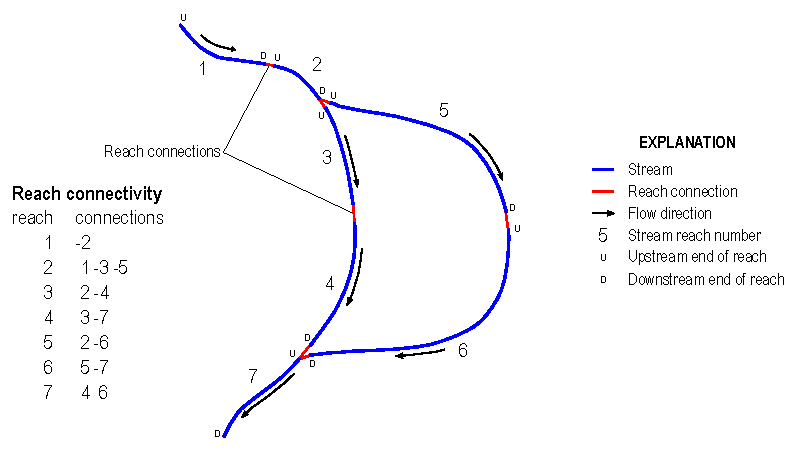
\includegraphics[scale=1.0]{sfr-connectivity}
	\caption[Illustration of a simple stream network having seven reaches with a junction having two reaches, a confluence of two reaches, and the resulting reach connectivity]{Simple stream network having seven reaches with a junction having two reaches, a confluence of two reaches, and the resulting reach connectivity. Downstream connections for a reach must include the reach as an upstream connection for all downstream connections to the reach. Downstream connections for a  reach are denoted with a negative reach number}
	\label{fig:sfr-connectivity}
\end{figure}


\vspace{5mm}
\subsubsection{Structure of Blocks}
\vspace{5mm}

\noindent \textit{FOR EACH SIMULATION}
\lstinputlisting[style=blockdefinition]{./mf6ivar/tex/gwf-sfr-options.dat}
\lstinputlisting[style=blockdefinition]{./mf6ivar/tex/gwf-sfr-dimensions.dat}
\lstinputlisting[style=blockdefinition]{./mf6ivar/tex/gwf-sfr-packagedata.dat}
\lstinputlisting[style=blockdefinition]{./mf6ivar/tex/gwf-sfr-connectiondata.dat}
\noindent \textit{IF \texttt{ndv} IS GREATER THAN ZERO FOR ANY REACH}
\lstinputlisting[style=blockdefinition]{./mf6ivar/tex/gwf-sfr-diversions.dat}

\vspace{5mm}
\noindent \textit{FOR ANY STRESS PERIOD}
\lstinputlisting[style=blockdefinition]{./mf6ivar/tex/gwf-sfr-period.dat}

\vspace{5mm}
\subsubsection{Explanation of Variables}
\begin{description}
% DO NOT MODIFY THIS FILE DIRECTLY.  IT IS CREATED BY mf6ivar.py 

\item \texttt{auxiliary}---defines an array of one or more auxiliary variable names.  There is no limit on the number of auxiliary variables that can be provided on this line; however, lists of information provided in subsequent blocks must have a column of data for each auxiliary variable name defined here.   The number of auxiliary variables detected on this line determines the value for naux.  Comments cannot be provided anywhere on this line as they will be interpreted as auxiliary variable names.  Auxiliary variables may not be used by the package, but they will be available for use by other parts of the program.  The program will terminate with an error if auxiliary variables are specified on more than one line in the options block.

\item \texttt{BOUNDNAMES}---keyword to indicate that boundary names may be provided with the list of stream reach cells.

\item \texttt{PRINT\_INPUT}---keyword to indicate that the list of stream reach information will be written to the listing file immediately after it is read.

\item \texttt{PRINT\_STAGE}---keyword to indicate that the list of stream reach stages will be printed to the listing file for every stress period in which ``HEAD PRINT'' is specified in Output Control.  If there is no Output Control option and \texttt{PRINT\_STAGE} is specified, then stages are printed for the last time step of each stress period.

\item \texttt{PRINT\_FLOWS}---keyword to indicate that the list of stream reach flow rates will be printed to the listing file for every stress period time step in which ``BUDGET PRINT'' is specified in Output Control.  If there is no Output Control option and \texttt{PRINT\_FLOWS} is specified, then flow rates are printed for the last time step of each stress period.

\item \texttt{SAVE\_FLOWS}---keyword to indicate that stream reach flow terms will be written to the file specified with ``BUDGET FILEOUT'' in Output Control.

\item \texttt{STAGE}---keyword to specify that record corresponds to stage.

\item \texttt{stagefile}---name of the binary output file to write stage information.

\item \texttt{BUDGET}---keyword to specify that record corresponds to the budget.

\item \texttt{FILEOUT}---keyword to specify that an output filename is expected next.

\item \texttt{budgetfile}---name of the binary output file to write budget information.

\item \texttt{TS6}---keyword to specify that record corresponds to a time-series file.

\item \texttt{FILEIN}---keyword to specify that an input filename is expected next.

\item \texttt{ts6\_filename}---defines a time-series file defining time series that can be used to assign time-varying values. See the ``Time-Variable Input'' section for instructions on using the time-series capability.

\item \texttt{OBS6}---keyword to specify that record corresponds to an observations file.

\item \texttt{obs6\_filename}---name of input file to define observations for the SFR package. See the ``Observation utility'' section for instructions for preparing observation input files. Table \ref{table:obstype} lists observation type(s) supported by the SFR package.

\item \texttt{MOVER}---keyword to indicate that this instance of the SFR Package can be used with the Water Mover (MVR) Package.  When the \texttt{MOVER} option is specified, additional memory is allocated within the package to store the available, provided, and received water.

\item \texttt{maximum\_iterations}---value that defines an maximum number of Streamflow Routing Newton-Raphson iterations allowed for a reach. By default, \texttt{maxsfrit} is equal to 100.

\item \texttt{maximum\_depth\_change}---value that defines the depth closure tolerance. By default, \texttt{dmaxchg} is equal to $1 \times 10^{-5}$.

\item \texttt{unit\_conversion}---value (or conversion factor) that is used in calculating stream depth for stream reach. A constant of 1.486 is used for flow units of cubic feet per second, and a constant of 1.0 is used for units of cubic meters per second. The constant must be multiplied by 86,400 when using time units of days in the simulation.

\item \texttt{maxbound}---integer value specifying the maximum number of stream reach cells that will be specified for use during any stress period.

\item \texttt{rno}---integer value that defines the reach number associated with the specified data on the line. \texttt{rno} must be greater than zero and less than or equal to \texttt{MAXBOUND}.

\item \texttt{cellid}---The keyword \texttt{`none'} must be specified for reaches that are not connected to an underlying GWF cell. The keyword \texttt{`none'} is used for reaches that are in cells that have \texttt{IDOMAIN} values less than one or are in areas not covered by the GWF model grid. Reach-aquifer flow is not calculated if the keyword \texttt{`none'} is specified.

\item \texttt{rlen}---real value that defines the reach length. \texttt{rlen} must be greater than zero.

\item \texttt{rwid}---real value that defines the reach width. \texttt{rwid} must be greater than zero.

\item \texttt{rgrd}---real value that defines the stream gradient (slope) across the reach. \texttt{rgrd} must be greater than zero.

\item \texttt{rtp}---real value that defines the top elevation of the reach streambed.

\item \texttt{rbth}---real value that defines the thickness of the reach streambed. \texttt{rbth} can be any value if \texttt{cellid} is \texttt{`none'}. Otherwise, \texttt{rbth} must be greater than zero.

\item \texttt{rhk}---real value that defines the hydraulic conductivity of the reach streambed. \texttt{rhk} can be any positive value if \texttt{cellid} is \texttt{`none'}. Otherwise, \texttt{rhk} must be greater than zero.

\item \textcolor{blue}{\texttt{man}---real or character value that defines the Manning's roughness coefficient for the reach. \texttt{man} must be greater than zero.  If the Options block includes a \texttt{TIMESERIESFILE} entry (see the ``Time-Variable Input'' section), values can be obtained from a time series by entering the time-series name in place of a numeric value.}

\item \texttt{ncon}---integer value that defines the number of reaches connected to the reach.

\item \texttt{ustrf}---real value that defines the fraction of upstream flow from each upstream reach that is applied as upstream inflow to the reach. The sum of all \texttt{ustrf} values for all reaches connected to the same upstream reach must be equal to one and \texttt{ustrf} must be greater than or equal to zero.

\item \texttt{ndv}---integer value that defines the number of downstream diversions for the reach.

\item \textcolor{blue}{\texttt{aux}---represents the values of the auxiliary variables for each stream reach. The values of auxiliary variables must be present for each stream reach. The values must be specified in the order of the auxiliary variables specified in the OPTIONS block.  If the package supports time series and the Options block includes a TIMESERIESFILE entry (see the ``Time-Variable Input'' section), values can be obtained from a time series by entering the time-series name in place of a numeric value.}

\item \texttt{boundname}---name of the stream reach cell.  \texttt{boundname} is an ASCII character variable that can contain as many as 40 characters.  If \texttt{boundname} contains spaces in it, then the entire name must be enclosed within single quotes.

\item \texttt{rno}---integer value that defines the reach number associated with the specified data on the line. \texttt{rno} must be greater than zero and less than or equal to \texttt{MAXBOUND}.

\item \texttt{ic}---integer value that defines the reach number of the reach connected to the current reach and whether it is connected to the upstream or downstream end of the reach. Negative \texttt{ic} numbers indicate connected reaches are connected to the downstream end of the current reach. Positive \texttt{ic} numbers indicate connected reaches are connected to the upstream end of the current reach. The absolute value of \texttt{ic} must be greater than zero and less than or equal to \texttt{MAXBOUND}.

\item \texttt{rno}---integer value that defines the reach number associated with the specified data on the line. \texttt{rno} must be greater than zero and less than or equal to \texttt{MAXBOUND}.

\item \texttt{idv}---integer value that defines the downstream diversion number for the diversion for reach \texttt{rno}. \texttt{idv} must be greater than zero and less than or equal to \texttt{ndv} for reach \texttt{rno}.

\item \texttt{iconr}---integer value that defines the downstream reach that will receive the diverted water. \texttt{idv} must be greater than zero and less than or equal to \texttt{MAXBOUND}. Furthermore, reach  \texttt{iconr} must be a downstream connection for reach \texttt{rno}.

\item \texttt{cprior}---character string value that defines the the prioritization system for the diversion, such as when insufficient water is available to meet all diversion stipulations, and is used in conjunction with the value of \texttt{flow} value specified in the \texttt{STRESS\_PERIOD\_DATA} section. Available diversion options include:  (1) \texttt{cprior} = `FRACTION', then the amount of the diversion is computed as a fraction of the streamflow leaving reach \texttt{rno} ($Q_{DS}$); in this case, 0.0 $\le$ \texttt{divflow} $\le$ 1.0.  (2) \texttt{cprior} = `EXCESS', a diversion is made only if $Q_{DS}$ for reach \texttt{rno} exceeds the value of \texttt{divflow}. If this occurs, then the quantity of water diverted is the excess flow ($Q_{DS} -$ \texttt{divflow}) and $Q_{DS}$ from reach \texttt{rno} is set equal to \texttt{divflow}. This represents a flood-control type of diversion, as described by Danskin and Hanson (2002). (3) \texttt{cprior} = `THRESHOLD', then if $Q_{DS}$ in reach \texttt{rno} is less than the specified diversion flow (\texttt{divflow}), no water is diverted from reach \texttt{rno}. If $Q_{DS}$ in reach \texttt{rno} is greater than or equal to (\texttt{divflow}), (\texttt{divflow}) is diverted and $Q_{DS}$ is set to the remainder ($Q_{DS} -$ \texttt{divflow})). This approach assumes that once flow in the stream is sufficiently low, diversions from the stream cease, and is the `priority' algorithm that originally was programmed into the STR1 Package (Prudic, 1989).  (4) \texttt{cprior} = `UPTO' -- if $Q_{DS}$ in reach \texttt{rno} is greater than or equal to the specified diversion flow (\texttt{divflow}), $Q_{DS}$ is reduced by \texttt{divflow}. If $Q_{DS}$ in reach \texttt{rno} is less than (\texttt{divflow}), \texttt{divflow} is set to $Q_{DS}$ and there will be no flow available for reaches connected to downstream end of reach \texttt{rno}.

\item \texttt{iper}---integer value specifying the starting stress period number for which the data specified in the PERIOD block apply.  \texttt{iper} must be less than \texttt{nper} in the TDIS Package and greater than zero.  The \texttt{iper} value assigned to a stress period block must be greater than the \texttt{iper} value assigned for the previous block.

\item \texttt{rno}---integer value that defines the reach number associated with the specified data on the line. \texttt{rno} must be greater than zero and less than or equal to \texttt{MAXBOUND}.

\item \texttt{sfrsetting}---line of information that is parsed into a keyword and values.  Keyword values that can be used to start the \texttt{sfrsetting} string include: \texttt{STATUS}, \texttt{MANNING}, \texttt{STAGE}, \texttt{INFLOW}, \texttt{RAINFALL}, \texttt{EVAPORATION}, \texttt{RUNOFF}, \texttt{DIVERSION}, \texttt{UPSTREAM\_FRACTION}, and \texttt{AUXILIARY}.

\begin{lstlisting}[style=blockdefinition]
STATUS <status>
MANNING <@manning@>
STAGE <@stage@>
INFLOW <@inflow@>
RAINFALL <@rainfall@>
EVAPORATION <@evaporation@>
RUNOFF <@runoff@>
DIVERSION <idv> <@divrate@> 
UPSTREAM_FRACTION <upstream_fraction>
AUXILIARY <auxname> <@auxval@> 
\end{lstlisting}

\item \texttt{status}---keyword option to define stream reach status.  \texttt{status} can be \texttt{ACTIVE}, \texttt{INACTIVE}, or \texttt{SIMPLE}. The \texttt{SIMPLE} \texttt{status} option simulates streamflow using a user-specified stage for a reach or a stage set to the top of the reach (depth = 0). In cases where the simulated leakage calculated using the specified stage exceeds the sum of inflows to the reach, the stage is set to the top of the reach and leakage is set equal to the sum of inflows. Upstream factions should be changed using the \texttt{UPSTREAM\_FRACTION} \texttt{sfrsetting} if the status for one or more reaches is changed to \texttt{ACTIVE} or \texttt{INACTIVE}. For example, if one of two downstream connections for a reach is inactivated, the upstream fraction for the active and inactive downstream reach should be changed to 1.0 and 0.0, respectively, to ensure that the active reach receives all of the downstream outflow from the upstream reach. By default, \texttt{status} is \texttt{ACTIVE}.

\item \textcolor{blue}{\texttt{manning}---real or character value that defines the Manning's roughness coefficient for the reach. \texttt{manning} must be greater than zero.  If the Options block includes a \texttt{TIMESERIESFILE} entry (see the ``Time-Variable Input'' section), values can be obtained from a time series by entering the time-series name in place of a numeric value.}

\item \textcolor{blue}{\texttt{stage}---real or character value that defines the stage for the reach. The specified \texttt{stage} is only applied if the reach uses the simple routing option. If \texttt{STAGE} is not specified for reaches that use the simple routing option, the specified stage is set to the top of the reach. If the Options block includes a \texttt{TIMESERIESFILE} entry (see the ``Time-Variable Input'' section), values can be obtained from a time series by entering the time-series name in place of a numeric value.}

\item \textcolor{blue}{\texttt{inflow}---real or character value that defines the volumetric inflow rate for the streamflow routing reach. If the Options block includes a TIMESERIESFILE entry (see the ``Time-Variable Input'' section), values can be obtained from a time series by entering the time-series name in place of a numeric value. By default, inflow rates are zero for each reach.}

\item \textcolor{blue}{\texttt{rainfall}---real or character value that defines the  volumetric rate per unit area of water added by precipitation directly on the streamflow routing reach. If the Options block includes a TIMESERIESFILE entry (see the ``Time-Variable Input'' section), values can be obtained from a time series by entering the time-series name in place of a numeric value. By default, rainfall  rates are zero for each reach.}

\item \textcolor{blue}{\texttt{evaporation}---real or character value that defines the  volumetric rate per unit area of water subtracted by evaporation from the streamflow routing reach. A positive evaporation rate should be provided. If the Options block includes a TIMESERIESFILE entry (see the ``Time-Variable Input'' section), values can be obtained from a time series by entering the time-series name in place of a numeric value. By default, evaporation rates are zero for each reach.}

\item \textcolor{blue}{\texttt{runoff}---real or character value that defines the volumetric rate of diffuse overland runoff that enters the streamflow routing reach. If the Options block includes a TIMESERIESFILE entry (see the ``Time-Variable Input'' section), values can be obtained from a time series by entering the time-series name in place of a numeric value. By default, runoff rates are zero for each reach.}

\item \texttt{DIVERSION}---keyword to indicate diversion record.

\item \texttt{idv}---diversion number.

\item \textcolor{blue}{\texttt{divrate}---real or character value that defines the volumetric diversion (\texttt{divflow}) rate for the streamflow routing reach. If the Options block includes a TIMESERIESFILE entry (see the ``Time-Variable Input'' section), values can be obtained from a time series by entering the time-series name in place of a numeric value.}

\item \texttt{upstream\_fraction}---real value that defines the fraction of upstream flow (\texttt{ustrf}) from each upstream reach that is applied as upstream inflow to the reach. The sum of all \texttt{ustrf} values for all reaches connected to the same upstream reach must be equal to one.

\item \texttt{AUXILIARY}---keyword for specifying auxiliary variable.

\item \texttt{auxname}---name for the auxiliary variable to be assigned \texttt{auxval}.  \texttt{auxname} must match one of the auxiliary variable names defined in the \texttt{OPTIONS} block. If \texttt{auxname} does not match one of the auxiliary variable names defined in the \texttt{OPTIONS} block the data are ignored.

\item \textcolor{blue}{\texttt{auxval}---value for the auxiliary variable.  If the Options block includes a TIMESERIESFILE entry (see the ``Time-Variable Input'' section), values can be obtained from a time series by entering the time-series name in place of a numeric value.}



\end{description}

\vspace{5mm}
\subsubsection{Example Input File}
\lstinputlisting[style=inputfile]{./mf6ivar/examples/gwf-sfr-example.dat}

\vspace{5mm}
\subsubsection{Available observation types}
Streamflow Routing Package observations include reach stage and all of the terms that contribute to the continuity equation for each stream reach. Additional SFR Package observations include the sum of inflows from upstream reaches and from mover terms (\texttt{upstream-flow}) and downstream outflow from a reach prior to diversions and the mover package (\texttt{downstream-flow}). The data required for each SFR Package observation type is defined in table~\ref{table:gwf-sfrobstype}. Negative and positive values for \texttt{sfr} observations represent a loss from and gain to the GWF model, respectively. For all other flow terms, negative and positive values represent a loss from and gain from the SFR package, respectively.

\FloatBarrier
\begin{longtable}{p{2cm} p{2.75cm} p{2cm} p{1.25cm} p{7cm}}
\caption{Available SFR Package observation types} \tabularnewline

\hline
\hline
\textbf{Stress Package} & \textbf{Observation type} & \textbf{ID} & \textbf{ID2} & \textbf{Description} \\
\hline
\endfirsthead

\captionsetup{textformat=simple}
\caption*{\textbf{Table \arabic{table}.}{\quad}Available SFR Package observation types.---Continued} \\

\hline
\hline
\textbf{Stress Package} & \textbf{Observation type} & \textbf{ID} & \textbf{ID2} & \textbf{Description} \\
\hline
\endhead


\hline
\endfoot

SFR & stage & rno or boundname & -- & Surface-water stage in a stream-reach boundary. If boundname is specified, boundname must be unique for each reach. \\
SFR & ext-inflow & rno or boundname & -- & Inflow into a stream-reach from an external boundary for a stream-reach or a group of stream-reaches. \\
SFR & inflow & rno or boundname & -- & Inflow into a stream-reach from upstream reaches for a stream-reach or a group of stream-reaches. \\
SFR & from-mvr & rno or boundname & -- & Inflow into a stream-reach from the MVR package for a stream-reach or a group of stream-reaches. \\
SFR & rainfall & rno or boundname & -- & Rainfall rate applied to a stream-reach or a group of stream-reaches. \\
SFR & runoff & rno or boundname & -- & Runoff rate applied to a stream-reach or a group of stream-reaches. \\
SFR & sfr & rno or boundname & -- & Simulated flow rate for a stream-reach and its aquifer connection for a stream-reach or a group of stream-reaches. \\
SFR & evaporation & rno or boundname & -- & Simulated evaporation rate from a stream-reach or a group of stream-reaches. \\
SFR & outflow & rno or boundname & -- & Outflow from a stream-reach to downstream reaches for a stream-reach or a group of stream-reaches. \\
SFR & ext-outflow & rno or boundname & -- & Outflow from a stream-reach to an external boundary for a stream-reach or a group of stream-reaches. \\
SFR & to-mvr & rno or boundname & -- & Outflow from a stream-reach that is available for the MVR package for a stream-reach or a group of stream-reaches. \\
SFR & upstream-flow & rno or boundname & -- & Upstream flow for a stream-reach or a group of stream-reaches from upstream reaches and the MVR package. \\
SFR & downstream-flow & rno or boundname & -- & Downstream flow for a stream-reach or a group of stream-reaches prior to diversions and the MVR package.

\label{table:gwf-sfrobstype}
\end{longtable}
\FloatBarrier

\vspace{5mm}
\subsubsection{Example Observation Input File}
\lstinputlisting[style=inputfile]{./mf6ivar/examples/gwf-sfr-example-obs.dat}


\newpage
\subsection{Lake (LAK) Package}
Input to the Lake (LAK) Package is read from the file that has type ``LAK6'' in the Name File.  Any number of LAK Packages can be specified for a single groundwater flow model.  All single valued variables are free format.

\vspace{5mm}
\subsubsection{Structure of Blocks}
\vspace{5mm}

\noindent \textit{FOR EACH SIMULATION}
\lstinputlisting[style=blockdefinition]{./mf6ivar/tex/gwf-lak-options.dat}
\lstinputlisting[style=blockdefinition]{./mf6ivar/tex/gwf-lak-dimensions.dat}
\lstinputlisting[style=blockdefinition]{./mf6ivar/tex/gwf-lak-packagedata.dat}
\noindent \textit{IF \texttt{nlakeconn} IS GREATER THAN ZERO FOR ANY LAKE}
\lstinputlisting[style=blockdefinition]{./mf6ivar/tex/gwf-lak-connectiondata.dat}
\noindent \textit{IF \texttt{ntables} IS GREATER THAN ZERO}
\lstinputlisting[style=blockdefinition]{./mf6ivar/tex/gwf-lak-tables.dat}
\noindent \textit{IF \texttt{noutlets} IS GREATER THAN ZERO FOR ANY LAKE}
\lstinputlisting[style=blockdefinition]{./mf6ivar/tex/gwf-lak-outlets.dat}

\vspace{5mm}
\noindent \textit{FOR ANY STRESS PERIOD}
\lstinputlisting[style=blockdefinition]{./mf6ivar/tex/gwf-lak-period.dat}

\vspace{5mm}
\subsubsection{Explanation of Variables}
\begin{description}
% DO NOT MODIFY THIS FILE DIRECTLY.  IT IS CREATED BY mf6ivar.py 

\item \textbf{Block: OPTIONS}

\begin{description}
\item \texttt{auxiliary}---defines an array of one or more auxiliary variable names.  There is no limit on the number of auxiliary variables that can be provided on this line; however, lists of information provided in subsequent blocks must have a column of data for each auxiliary variable name defined here.   The number of auxiliary variables detected on this line determines the value for naux.  Comments cannot be provided anywhere on this line as they will be interpreted as auxiliary variable names.  Auxiliary variables may not be used by the package, but they will be available for use by other parts of the program.  The program will terminate with an error if auxiliary variables are specified on more than one line in the options block.

\item \texttt{BOUNDNAMES}---keyword to indicate that boundary names may be provided with the list of lake cells.

\item \texttt{PRINT\_INPUT}---keyword to indicate that the list of lake information will be written to the listing file immediately after it is read.

\item \texttt{PRINT\_STAGE}---keyword to indicate that the list of lake stages will be printed to the listing file for every stress period in which ``HEAD PRINT'' is specified in Output Control.  If there is no Output Control option and PRINT\_STAGE is specified, then stages are printed for the last time step of each stress period.

\item \texttt{PRINT\_FLOWS}---keyword to indicate that the list of lake flow rates will be printed to the listing file for every stress period time step in which ``BUDGET PRINT'' is specified in Output Control.  If there is no Output Control option and ``PRINT\_FLOWS'' is specified, then flow rates are printed for the last time step of each stress period.

\item \texttt{SAVE\_FLOWS}---keyword to indicate that lake flow terms will be written to the file specified with ``BUDGET FILEOUT'' in Output Control.

\item \texttt{STAGE}---keyword to specify that record corresponds to stage.

\item \texttt{stagefile}---name of the binary output file to write stage information.

\item \texttt{BUDGET}---keyword to specify that record corresponds to the budget.

\item \texttt{FILEOUT}---keyword to specify that an output filename is expected next.

\item \texttt{budgetfile}---name of the binary output file to write budget information.

\item \texttt{TS6}---keyword to specify that record corresponds to a time-series file.

\item \texttt{FILEIN}---keyword to specify that an input filename is expected next.

\item \texttt{ts6\_filename}---defines a time-series file defining time series that can be used to assign time-varying values. See the ``Time-Variable Input'' section for instructions on using the time-series capability.

\item \texttt{OBS6}---keyword to specify that record corresponds to an observations file.

\item \texttt{obs6\_filename}---name of input file to define observations for the LAK package. See the ``Observation utility'' section for instructions for preparing observation input files. Table \ref{table:obstype} lists observation type(s) supported by the LAK package.

\item \texttt{MOVER}---keyword to indicate that this instance of the LAK Package can be used with the Water Mover (MVR) Package.  When the MOVER option is specified, additional memory is allocated within the package to store the available, provided, and received water.

\item \texttt{surfdep}---real value that defines the surface depression depth for VERTICAL lake-GWF connections. If specified, SURFDEP must be greater than or equal to zero. If SURFDEP is not specified, a default value of zero is used for all vertical lake-GWF connections.

\item \texttt{time\_conversion}---value that is used in converting outlet flow terms that use Manning's equation or gravitational acceleration to consistent time units. TIME\_CONVERSION should be set to 1.0, 60.0, 3,600.0, 86,400.0, and 31,557,600.0 when using time units (TIME\_UNITS) of seconds, minutes, hours, days, or years in the simulation, respectively. CONVTIME does not need to be specified if no lake outlets are specified or TIME\_UNITS are seconds.

\item \texttt{length\_conversion}---real value that is used in converting outlet flow terms that use Manning's equation or gravitational acceleration to consistent length units. LENGTH\_CONVERSION should be set to 3.28081, 1.0, and 100.0 when using length units (LENGTH\_UNITS) of feet, meters, or centimeters in the simulation, respectively. LENGTH\_CONVERSION does not need to be specified if no lake outlets are specified or LENGTH\_UNITS are meters.

\end{description}
\item \textbf{Block: DIMENSIONS}

\begin{description}
\item \texttt{nlakes}---value specifying the number of lakes that will be simulated for all stress periods.

\item \texttt{noutlets}---value specifying the number of outlets that will be simulated for all stress periods. If NOUTLETS is not specified, a default value of zero is used.

\item \texttt{ntables}---value specifying the number of lakes tables that will be used to define the lake stage, volume relation, and surface area. If NTABLES is not specified, a default value of zero is used.

\end{description}
\item \textbf{Block: PACKAGEDATA}

\begin{description}
\item \texttt{lakeno}---integer value that defines the lake number associated with the specified PACKAGEDATA data on the line. LAKENO must be greater than zero and less than or equal to NLAKES. Lake information must be specified for every lake or the program will terminate with an error.  The program will also terminate with an error if information for a lake is specified more than once.

\item \texttt{strt}---real value that defines the starting stage for the lake.

\item \texttt{nlakeconn}---integer value that defines the number of GWF cells connected to this (LAKENO) lake. There can only be one vertical lake connection to each GWF cell. NLAKECONN must be greater than zero.

\item \textcolor{blue}{\texttt{aux}---represents the values of the auxiliary variables for each lake. The values of auxiliary variables must be present for each lake. The values must be specified in the order of the auxiliary variables specified in the OPTIONS block.  If the package supports time series and the Options block includes a TIMESERIESFILE entry (see the ``Time-Variable Input'' section), values can be obtained from a time series by entering the time-series name in place of a numeric value.}

\item \texttt{boundname}---name of the lake cell.  BOUNDNAME is an ASCII character variable that can contain as many as 40 characters.  If BOUNDNAME contains spaces in it, then the entire name must be enclosed within single quotes.

\end{description}
\item \textbf{Block: CONNECTIONDATA}

\begin{description}
\item \texttt{lakeno}---integer value that defines the lake number associated with the specified CONNECTIONDATA data on the line. LAKENO must be greater than zero and less than or equal to NLAKES. Lake connection information must be specified for every lake connection to the GWF model (NLAKECONN) or the program will terminate with an error.  The program will also terminate with an error if connection information for a lake connection to the GWF model is specified more than once.

\item \texttt{iconn}---integer value that defines the GWF connection number for this lake connection entry. ICONN must be greater than zero and less than or equal to NLAKECONN for lake LAKENO.

\item \texttt{cellid}---is the cell identifier, and depends on the type of grid that is used for the simulation.  For a structured grid that uses the DIS input file, CELLID is the layer, row, and column.   For a grid that uses the DISV input file, CELLID is the layer and CELL2D number.  If the model uses the unstructured discretization (DISU) input file, CELLID is the node number for the cell.

\item \texttt{claktype}---character string that defines the lake-GWF connection type for the lake connection. Possible lake-GWF connection type strings include:  VERTICAL--character keyword to indicate the lake-GWF connection is vertical  and connection conductance calculations use the hydraulic conductivity corresponding to the $K_{33}$ tensor component defined for CELLID in the NPF package. HORIZONTAL--character keyword to indicate the lake-GWF connection is horizontal and connection conductance calculations use the hydraulic conductivity corresponding to the $K_{11}$ tensor component defined for CELLID in the NPF package. EMBEDDEDH--character keyword to indicate the lake-GWF connection is embedded in a single cell and connection conductance calculations use the hydraulic conductivity corresponding to the $K_{11}$ tensor component defined for CELLID in the NPF package. EMBEDDEDV--character keyword to indicate the lake-GWF connection is embedded in a single cell and connection conductance calculations use the hydraulic conductivity corresponding to the $K_{33}$ tensor component defined for CELLID in the NPF package. Embedded lakes can only be connected to a single cell (NLAKCONN = 1) and there must be a lake table associated with each embedded lake.

\item \texttt{bedleak}---character string or real value that defines the bed leakance for the lake-GWF connection. BEDLEAK must be greater than or equal to zero or specified to be NONE. If BEDLEAK is specified to be NONE, the lake-GWF connection conductance is solely a function of aquifer properties in the connected GWF cell and lakebed sediments are assumed to be absent.

\item \texttt{belev}---real value that defines the bottom elevation for a HORIZONTAL lake-GWF connection. Any value can be specified if CLAKTYPE is VERTICAL, EMBEDDEDH, or EMBEDDEDV. If CLAKTYPE is HORIZONTAL and BELEV is not equal to TELEV, BELEV must be greater than or equal to the bottom of the GWF cell CELLID. If BELEV is equal to TELEV, BELEV is reset to the bottom of the GWF cell CELLID.

\item \texttt{telev}---real value that defines the top elevation for a HORIZONTAL lake-GWF connection. Any value can be specified if CLAKTYPE is VERTICAL, EMBEDDEDH, or EMBEDDEDV. If CLAKTYPE is HORIZONTAL and TELEV is not equal to BELEV, TELEV must be less than or equal to the top of the GWF cell CELLID. If TELEV is equal to BELEV, TELEV is reset to the top of the GWF cell CELLID.

\item \texttt{connlen}---real value that defines the distance between the connected GWF CELLID node and the lake for a HORIZONTAL, EMBEDDEDH, or EMBEDDEDV lake-GWF connection. CONLENN must be greater than zero for a HORIZONTAL, EMBEDDEDH, or EMBEDDEDV lake-GWF connection. Any value can be specified if CLAKTYPE is VERTICAL.

\item \texttt{connwidth}---real value that defines the connection face width for a HORIZONTAL lake-GWF connection. CONNWIDTH must be greater than zero for a HORIZONTAL lake-GWF connection. Any value can be specified if CLAKTYPE is VERTICAL, EMBEDDEDH, or EMBEDDEDV.

\end{description}
\item \textbf{Block: TABLES}

\begin{description}
\item \texttt{lakeno}---integer value that defines the lake number associated with the specified TABLES data on the line. LAKENO must be greater than zero and less than or equal to NLAKES. The program will terminate with an error if table information for a lake is specified more than once or the number of specified tables is less than NTABLES.

\item \texttt{TAB6}---keyword to specify that record corresponds to a table file.

\item \texttt{FILEIN}---keyword to specify that an input filename is expected next.

\item \texttt{tab6\_filename}---character string that defines the path and filename for the file containing lake table data for the lake connection. The CTABNAME file includes the number of entries in the file and the relation between stage, surface area, and volume for each entry in the file. Lake table files for EMBEDDEDH and EMBEDDEDV lake-GWF connections also include lake-GWF exchange area data for each entry in the file. Input instructions for the CTABNAME file is included at the LAK package lake table file input instructions section.

\end{description}
\item \textbf{Block: OUTLETS}

\begin{description}
\item \texttt{outletno}---integer value that defines the outlet number associated with the specified OUTLETS data on the line. OUTLETNO must be greater than zero and less than or equal to NOUTLETS. Outlet information must be specified for every outlet or the program will terminate with an error. The program will also terminate with an error if information for a outlet is specified more than once.

\item \texttt{lakein}---integer value that defines the lake number that outlet is connected to. LAKEIN must be greater than zero and less than or equal to NLAKES.

\item \texttt{lakeout}---integer value that defines the lake number that outlet discharge from lake outlet OUTLETNO is routed to. LAKEOUT must be greater than or equal to zero and less than or equal to NLAKES. If LAKEOUT is zero, outlet discharge from lake outlet OUTLETNO is discharged to an external boundary.

\item \texttt{couttype}---character string that defines the outlet type for the outlet OUTLETNO. Possible COUTTYPE strings include: SPECIFIED--character keyword to indicate the outlet is defined as a specified flow.  MANNING--character keyword to indicate the outlet is defined using Manning's equation. WEIR--character keyword to indicate the outlet is defined using a sharp weir equation.

\item \textcolor{blue}{\texttt{invert}---real value that defines the invert elevation for the lake outlet. Any value can be specified if COUTTYPE is SPECIFIED. If the Options block includes a TIMESERIESFILE entry (see the ``Time-Variable Input'' section), values can be obtained from a time series by entering the time-series name in place of a numeric value.}

\item \textcolor{blue}{\texttt{width}---real value that defines the width of the lake outlet. Any value can be specified if COUTTYPE is SPECIFIED. If the Options block includes a TIMESERIESFILE entry (see the ``Time-Variable Input'' section), values can be obtained from a time series by entering the time-series name in place of a numeric value.}

\item \textcolor{blue}{\texttt{rough}---real value that defines the roughness coefficient for the lake outlet. Any value can be specified if COUTTYPE is not MANNING. If the Options block includes a TIMESERIESFILE entry (see the ``Time-Variable Input'' section), values can be obtained from a time series by entering the time-series name in place of a numeric value.}

\item \textcolor{blue}{\texttt{slope}---real value that defines the bed slope for the lake outlet. Any value can be specified if COUTTYPE is not MANNING. If the Options block includes a TIMESERIESFILE entry (see the ``Time-Variable Input'' section), values can be obtained from a time series by entering the time-series name in place of a numeric value.}

\end{description}
\item \textbf{Block: PERIOD}

\begin{description}
\item \texttt{iper}---integer value specifying the starting stress period number for which the data specified in the PERIOD block apply.  IPER must be less than or equal to NPER in the TDIS Package and greater than zero.  The IPER value assigned to a stress period block must be greater than the IPER value assigned for the previous PERIOD block.  The information specified in the PERIOD block will continue to apply for all subsequent stress periods, unless the program encounters another PERIOD block.

\item \texttt{lakeno}---integer value that defines the lake number associated with the specified PERIOD data on the line. LAKENO must be greater than zero and less than or equal to NLAKES.

\item \texttt{laksetting}---line of information that is parsed into a keyword and values.  Keyword values that can be used to start the LAKSETTING string include: STATUS, STAGE, STAGE, EVAPORATION, RUNOFFON, WITHDRAWAL, and AUXILIARY.

\begin{lstlisting}[style=blockdefinition]
STATUS <status>
STAGE <@stage@>
RAINFALL <@rainfall@>
EVAPORATION <@evaporation@>
RUNOFF <@runoff@>
WITHDRAWAL <@withdrawal@>
AUXILIARY <auxname> <@auxval@> 
\end{lstlisting}

\item \texttt{status}---keyword option to define lake status.  STATUS can be ACTIVE, INACTIVE, or CONSTANT. By default, STATUS is ACTIVE.

\item \textcolor{blue}{\texttt{stage}---real or character value that defines the stage for the lake. The specified STAGE is only applied if the lake is a constant stage lake. If the Options block includes a TIMESERIESFILE entry (see the ``Time-Variable Input'' section), values can be obtained from a time series by entering the time-series name in place of a numeric value.}

\item \textcolor{blue}{\texttt{rainfall}---real or character value that defines the rainfall rate $(LT^{-1})$ for the lake. Value must be greater than or equal to zero. If the Options block includes a TIMESERIESFILE entry (see the ``Time-Variable Input'' section), values can be obtained from a time series by entering the time-series name in place of a numeric value.}

\item \textcolor{blue}{\texttt{evaporation}---real or character value that defines the maximum evaporation rate $(LT^{-1})$ for the lake. Value must be greater than or equal to zero. If the Options block includes a TIMESERIESFILE entry (see the ``Time-Variable Input'' section), values can be obtained from a time series by entering the time-series name in place of a numeric value.}

\item \textcolor{blue}{\texttt{runoff}---real or character value that defines the runoff rate $(L^3 T^{-1})$ for the lake. Value must be greater than or equal to zero. If the Options block includes a TIMESERIESFILE entry (see the ``Time-Variable Input'' section), values can be obtained from a time series by entering the time-series name in place of a numeric value.}

\item \textcolor{blue}{\texttt{withdrawal}---real or character value that defines the maximum withdrawal rate $(L^3 T^{-1})$ for the lake. Value must be greater than or equal to zero. If the Options block includes a TIMESERIESFILE entry (see the ``Time-Variable Input'' section), values can be obtained from a time series by entering the time-series name in place of a numeric value.}

\item \texttt{AUXILIARY}---keyword for specifying auxiliary variable.

\item \texttt{auxname}---name for the auxiliary variable to be assigned AUXVAL.  AUXNAME must match one of the auxiliary variable names defined in the OPTIONS block. If AUXNAME does not match one of the auxiliary variable names defined in the OPTIONS block the data are ignored.

\item \textcolor{blue}{\texttt{auxval}---value for the auxiliary variable. If the Options block includes a TIMESERIESFILE entry (see the ``Time-Variable Input'' section), values can be obtained from a time series by entering the time-series name in place of a numeric value.}

\item \texttt{outletno}---integer value that defines the outlet number associated with the specified PERIOD data on the line. OUTLETNO must be greater than zero and less than or equal to NOUTLETS.

\item \texttt{outletsetting}---line of information that is parsed into a keyword and values.  Keyword values that can be used to start the OUTLETSETTING string include: RATE, INVERT, WIDTH, SLOPE, and ROUGH.

\begin{lstlisting}[style=blockdefinition]
RATE <@rate@>
INVERT <@invert@>
WIDTH <@width@>
SLOPE <@slope@>
ROUGH <@rough@>
\end{lstlisting}

\item \textcolor{blue}{\texttt{rate}---real or character value that defines the extraction rate for the lake outflow. A positive value indicates inflow and a negative value indicates outflow from the lake. RATE only applies to active (IBOUND $>$ 0) lakes. A specified RATE is only applied if COUTTYPE for the OUTLETNO is SPECIFIED. If the Options block includes a TIMESERIESFILE entry (see the ``Time-Variable Input'' section), values can be obtained from a time series by entering the time-series name in place of a numeric value. By default, the RATE for each SPECIFIED lake outlet is zero.}

\item \textcolor{blue}{\texttt{invert}---real or character value that defines the invert elevation for the lake outlet. A specified INVERT value is only used for active lakes if COUTTYPE for lake outlet OUTLETNO is not SPECIFIED. If the Options block includes a TIMESERIESFILE entry (see the ``Time-Variable Input'' section), values can be obtained from a time series by entering the time-series name in place of a numeric value.}

\item \textcolor{blue}{\texttt{rough}---real or character value that defines the width of the lake outlet. A specified WIDTH value is only used for active lakes if COUTTYPE for lake outlet OUTLETNO is not SPECIFIED. If the Options block includes a TIMESERIESFILE entry (see the ``Time-Variable Input'' section), values can be obtained from a time series by entering the time-series name in place of a numeric value.}

\item \textcolor{blue}{\texttt{width}---real or character value that defines the width of the lake outlet. A specified WIDTH value is only used for active lakes if COUTTYPE for lake outlet OUTLETNO is not SPECIFIED. If the Options block includes a TIMESERIESFILE entry (see the ``Time-Variable Input'' section), values can be obtained from a time series by entering the time-series name in place of a numeric value.}

\item \textcolor{blue}{\texttt{slope}---real or character value that defines the bed slope for the lake outlet. A specified SLOPE value is only used for active lakes if COUTTYPE for lake outlet OUTLETNO is MANNING. If the Options block includes a TIMESERIESFILE entry (see the ``Time-Variable Input'' section), values can be obtained from a time series by entering the time-series name in place of a numeric value.}

\end{description}


\end{description}

\vspace{5mm}
\subsubsection{Example Input File}
\lstinputlisting[style=inputfile]{./mf6ivar/examples/gwf-lak-example.dat}

\vspace{5mm}
\subsubsection{Available observation types}
Lake Package observations include lake stage and all of the terms that contribute to the continuity equation for each lake. Additional LAK Package observations include flow rates for individual outlets, lakes, or groups of lakes (\texttt{outlet}); the lake volume (\texttt{volume}); lake surface area (\texttt{surface-area}); wetted area for a lake-aquifer connection (\texttt{wetted-area}); and the conductance for a lake-aquifer connection conductance (\texttt{conductance}). The data required for each LAK Package observation type is defined in table~\ref{table:gwf-lakobstype}. Negative and positive values for \texttt{lak} observations represent a loss from and gain to the GWF model, respectively. For all other flow terms, negative and positive values represent a loss from and gain from the LAK package, respectively.

\begin{longtable}{p{2cm} p{2.75cm} p{2cm} p{1.25cm} p{7cm}}
\caption{Available LAK Package observation types} \tabularnewline

\hline
\hline
\textbf{Stress Package} & \textbf{Observation type} & \textbf{ID} & \textbf{ID2} & \textbf{Description} \\
\hline
\endfirsthead

\captionsetup{textformat=simple}
\caption*{\textbf{Table \arabic{table}.}{\quad}Available LAK Package observation types.---Continued} \tabularnewline

\hline
\hline
\textbf{Stress Package} & \textbf{Observation type} & \textbf{ID} & \textbf{ID2} & \textbf{Description} \\
\hline
\endhead


\hline
\endfoot

LAK & stage & lakeno or boundname & -- & Surface-water stage in a lake. If boundname is specified, boundname must be unique for each lake. \\
LAK & ext-inflow & lakeno or boundname & -- & Specified inflow into a lake or group of lakes. \\
LAK & outlet-inflow & lakeno or boundname & -- & Simulated inflow from upstream lake outlets into a lake or group of lakes. \\
LAK & inflow & lakeno or boundname & -- & Sum of specified inflow and simulated inflow from upstream lake outlets into a lake or group of lakes. \\
LAK & from-mvr & lakeno or boundname & -- & Inflow into a lake or group of lakes from the MVR package. \\
LAK & rainfall & lakeno or boundname & -- & Rainfall rate applied to a lake or group of lakes. \\
LAK & runoff & lakeno or boundname & -- & Runoff rate applied to a lake or group of lakes. \\
LAK & lak & lakeno or boundname & \texttt{iconn} or -- & Simulated flow rate for a lake or group of lakes and its aquifer connection(s). If boundname is not specified for ID, then the simulated lake-aquifer flow rate at a specific lake connection is observed. In this case, ID2 must be specified and is the connection number \texttt{iconn}. \\
LAK & withdrawal & lakeno or boundname & -- & Specified withdrawal rate from a lake or group of lakes. \\
LAK & evaporation & lakeno or boundname & -- & Simulated evaporation rate from a lake or group of lakes. \\
LAK & ext-outflow & outletno or boundname & -- & External outflow from a lake outlet, a lake, or a group of lakes to an external boundary. If boundname is not specified for ID, then the external outflow from a specific lake outlet is observed. In this case, ID is the outlet number outletno. \\
LAK & to-mvr & outletno or boundname & -- & Outflow from a lake outlet, a lake, or a group of lakes that is available for the MVR package. If boundname is not specified for ID, then the outflow available for the MVR package from a specific lake outlet is observed. In this case, ID is the outlet number outletno. \\
LAK & storage & lakeno or boundname & -- & Simulated storage flow rate for a lake or group of lakes. \\
LAK & constant & lakeno or boundname & -- & Simulated constant-flow rate for a lake or group of lakes. \\
LAK & outlet & outletno or boundname & -- & Simulated outlet flow rate from a lake outlet, a lake, or a group of lakes. If boundname is not specified for ID, then the flow from a specific lake outlet is observed. In this case, ID is the outlet number outletno. \\
LAK & volume & lakeno or boundname & -- & Simulated lake volume or group of lakes. \\
LAK & surface-area & lakeno or boundname & -- & Simulated surface area for a lake or group of lakes. \\
LAK & wetted-area & lakeno or boundname & \texttt{iconn} or -- & Simulated wetted-area for a lake or group of lakes and its aquifer connection(s). If boundname is not specified for ID, then the wetted area of a specific lake connection is observed. In this case, ID2 must be specified and is the connection number \texttt{iconn}. \\
LAK & conductance & lakeno or boundname & \texttt{iconn} or -- & Calculated conductance for a lake or group of lakes and its aquifer connection(s). If boundname is not specified for ID, then the calculated conductance of a specific lake connection is observed. In this case, ID2 must be specified and is the connection number \texttt{iconn}.

\label{table:gwf-lakobstype}
\end{longtable}

\vspace{5mm}
\subsubsection{Example Observation Input File}
\lstinputlisting[style=inputfile]{./mf6ivar/examples/gwf-lak-example-obs.dat}

\newpage
\subsection{Lake Table Input File}
Lake tables of stage, volume, and surface area can be specified for individual lakes.  Lake tables are specified by including file names in the LAKE\_TABLES block of the LAK Package.  These file names correspond to a lake table input file.  The format of the lake table input file is described here.  All single valued variables are free format.

\vspace{5mm}
\subsubsection{Structure of Blocks}
\vspace{5mm}

\lstinputlisting[style=blockdefinition]{./mf6ivar/tex/gwf-laktab-dimensions.dat}
\lstinputlisting[style=blockdefinition]{./mf6ivar/tex/gwf-laktab-table.dat}
\vspace{5mm}

\vspace{5mm}
\subsubsection{Explanation of Variables}
\begin{description}
% DO NOT MODIFY THIS FILE DIRECTLY.  IT IS CREATED BY mf6ivar.py 

\item \textbf{Block: DIMENSIONS}

\begin{description}
\item \texttt{nrow}---integer value specifying the number of rows in the lake table. There must be \texttt{nrow} rows of data in the \texttt{TABLE} block.

\item \texttt{ncol}---integer value specifying the number of colums in the lake table. There must be \texttt{ncol} columns of data in the \texttt{TABLE} block. For lakes with \texttt{HORIZONTAL} and/or \texttt{VERTICAL} \texttt{ctype} connections, \texttt{NROW} must be equal to 3. For lakes with \texttt{EMBEDDEDH} or \texttt{EMBEDDEDV} \texttt{ctype} connections, \texttt{NROW} must be equal to 4.

\end{description}
\item \textbf{Block: TABLE}

\begin{description}
\item \texttt{stage}---real value that defines the stage corresponding to the remaining data on the line.

\item \texttt{volume}---real value that defines the lake volume corresponding to the stage specified on the line.

\item \texttt{sarea}---real value that defines the lake surface area corresponding to the stage specified on the line.

\item \texttt{barea}---real value that defines the lake-\texttt{GWF} exchange area corresponding to the stage specified on the line. \texttt{barea} is only specified if the \texttt{claktype} for the lake is \texttt{EMBEDDEDH} or \texttt{EMBEDDEDV}.

\end{description}


\end{description}

\subsubsection{Example Input File}
\lstinputlisting[style=inputfile]{./mf6ivar/examples/gwf-laktab-example.dat}



\newpage
\subsection{Unsaturated Zone Flow (UZF) Package}
Input to the Unsaturated Zone Flow (UZF) Package is read from the file that has type ``UZF6'' in the Name File.

\vspace{5mm}
\subsubsection{Structure of Blocks}
\vspace{5mm}

\noindent \textit{FOR EACH SIMULATION}
\lstinputlisting[style=blockdefinition]{./mf6ivar/tex/gwf-uzf-options.dat}
\lstinputlisting[style=blockdefinition]{./mf6ivar/tex/gwf-uzf-dimensions.dat}
\lstinputlisting[style=blockdefinition]{./mf6ivar/tex/gwf-uzf-packagedata.dat}

\vspace{5mm}
\noindent \textit{FOR ANY STRESS PERIOD}
\lstinputlisting[style=blockdefinition]{./mf6ivar/tex/gwf-uzf-period.dat}
\advancedpackageperioddescription{UZF cell}{UZF cells}

\vspace{5mm}
\subsubsection{Explanation of Variables}
\begin{description}
% DO NOT MODIFY THIS FILE DIRECTLY.  IT IS CREATED BY mf6ivar.py 

\item \textbf{Block: OPTIONS}

\begin{description}
\item \texttt{auxiliary}---defines an array of one or more auxiliary variable names.  There is no limit on the number of auxiliary variables that can be provided on this line; however, lists of information provided in subsequent blocks must have a column of data for each auxiliary variable name defined here.   The number of auxiliary variables detected on this line determines the value for naux.  Comments cannot be provided anywhere on this line as they will be interpreted as auxiliary variable names.  Auxiliary variables may not be used by the package, but they will be available for use by other parts of the program.  The program will terminate with an error if auxiliary variables are specified on more than one line in the options block.

\item \texttt{auxmultname}---name of auxiliary variable to be used as multiplier of GWF cell area used by UZF cell.

\item \texttt{BOUNDNAMES}---keyword to indicate that boundary names may be provided with the list of UZF cells.

\item \texttt{PRINT\_INPUT}---keyword to indicate that the list of UZF information will be written to the listing file immediately after it is read.

\item \texttt{PRINT\_FLOWS}---keyword to indicate that the list of UZF flow rates will be printed to the listing file for every stress period time step in which ``BUDGET PRINT'' is specified in Output Control.  If there is no Output Control option and ``PRINT\_FLOWS'' is specified, then flow rates are printed for the last time step of each stress period.

\item \texttt{SAVE\_FLOWS}---keyword to indicate that UZF flow terms will be written to the file specified with ``BUDGET FILEOUT'' in Output Control.

\item \texttt{BUDGET}---keyword to specify that record corresponds to the budget.

\item \texttt{FILEOUT}---keyword to specify that an output filename is expected next.

\item \texttt{budgetfile}---name of the binary output file to write budget information.

\item \texttt{PACKAGE\_CONVERGENCE}---keyword to specify that record corresponds to the package convergence comma spaced values file.

\item \texttt{package\_convergence\_filename}---name of the comma spaced values output file to write package convergence information.

\item \texttt{TS6}---keyword to specify that record corresponds to a time-series file.

\item \texttt{FILEIN}---keyword to specify that an input filename is expected next.

\item \texttt{ts6\_filename}---defines a time-series file defining time series that can be used to assign time-varying values. See the ``Time-Variable Input'' section for instructions on using the time-series capability.

\item \texttt{OBS6}---keyword to specify that record corresponds to an observations file.

\item \texttt{obs6\_filename}---name of input file to define observations for the UZF package. See the ``Observation utility'' section for instructions for preparing observation input files. Table \ref{table:obstype} lists observation type(s) supported by the UZF package.

\item \texttt{MOVER}---keyword to indicate that this instance of the UZF Package can be used with the Water Mover (MVR) Package.  When the MOVER option is specified, additional memory is allocated within the package to store the available, provided, and received water.

\item \texttt{SIMULATE\_ET}---keyword specifying that ET in the unsaturated (UZF) and saturated zones (GWF) will be simulated. ET can be simulated in the UZF cell and not the GWF cell by omitting keywords LINEAR\_GWET and SQUARE\_GWET.

\item \texttt{LINEAR\_GWET}---keyword specifying that groundwater ET will be simulated using the original ET formulation of MODFLOW-2005.

\item \texttt{SQUARE\_GWET}---keyword specifying that groundwater ET will be simulated by assuming a constant ET rate for groundwater levels between land surface (TOP) and land surface minus the ET extinction depth (TOP-EXTDP). Groundwater ET is smoothly reduced from the PET rate to zero over a nominal interval at TOP-EXTDP.

\item \texttt{SIMULATE\_GWSEEP}---keyword specifying that groundwater discharge (GWSEEP) to land surface will be simulated. Groundwater discharge is nonzero when groundwater head is greater than land surface.

\item \texttt{UNSAT\_ETWC}---keyword specifying that ET in the unsaturated zone will be simulated as a function of the specified PET rate while the water content (THETA) is greater than the ET extinction water content (EXTWC).

\item \texttt{UNSAT\_ETAE}---keyword specifying that ET in the unsaturated zone will be simulated simulated using a capillary pressure based formulation. Capillary pressure is calculated using the Brooks-Corey retention function.

\end{description}
\item \textbf{Block: DIMENSIONS}

\begin{description}
\item \texttt{nuzfcells}---is the number of UZF cells.  More than one UZF cell can be assigned to a GWF cell; however, only one GWF cell can be assigned to a single UZF cell. If more than one UZF cell is assigned to a GWF cell, then an auxiliary variable should be used to reduce the surface area of the UZF cell with the AUXMULTNAME option.

\item \texttt{ntrailwaves}---is the number of trailing waves.  A recommended value of 7 can be used for NTRAILWAVES.  This value can be increased to lower mass balance error in the unsaturated zone.

\item \texttt{nwavesets}---is the number of wave sets.  A recommended value of 40 can be used for NWAVESETS.  This value can be increased if more waves are required to resolve variations in water content within the unsaturated zone.

\end{description}
\item \textbf{Block: PACKAGEDATA}

\begin{description}
\item \texttt{iuzno}---integer value that defines the UZF cell number associated with the specified PACKAGEDATA data on the line. IUZNO must be greater than zero and less than or equal to NUZFCELLS.  UZF information must be specified for every UZF cell or the program will terminate with an error.  The program will also terminate with an error if information for a UZF cell is specified more than once.

\item \texttt{cellid}---is the cell identifier, and depends on the type of grid that is used for the simulation.  For a structured grid that uses the DIS input file, CELLID is the layer, row, and column.   For a grid that uses the DISV input file, CELLID is the layer and CELL2D number.  If the model uses the unstructured discretization (DISU) input file, CELLID is the node number for the cell.

\item \texttt{landflag}---integer value set to one for land surface cells indicating that boundary conditions can be applied and data can be specified in the PERIOD block. A value of 0 specifies a non-land surface cell.

\item \texttt{ivertcon}---integer value set to specify underlying UZF cell that receives water flowing to bottom of cell. If unsaturated zone flow reaches the water table before the cell bottom, then water is added to the GWF cell instead of flowing to the underlying UZF cell. A value of 0 indicates the UZF cell is not connected to an underlying UZF cell.

\item \texttt{surfdep}---is the surface depression depth of the UZF cell.

\item \texttt{vks}---is the vertical saturated hydraulic conductivity of the UZF cell.

\item \texttt{thtr}---is the residual (irreducible) water content of the UZF cell.

\item \texttt{thts}---is the saturated water content of the UZF cell.

\item \texttt{thti}---is the initial water content of the UZF cell.

\item \texttt{eps}---is the epsilon exponent of the UZF cell.

\item \texttt{boundname}---name of the UZF cell cell.  BOUNDNAME is an ASCII character variable that can contain as many as 40 characters.  If BOUNDNAME contains spaces in it, then the entire name must be enclosed within single quotes.

\end{description}
\item \textbf{Block: PERIOD}

\begin{description}
\item \texttt{iper}---integer value specifying the starting stress period number for which the data specified in the PERIOD block apply.  IPER must be less than or equal to NPER in the TDIS Package and greater than zero.  The IPER value assigned to a stress period block must be greater than the IPER value assigned for the previous PERIOD block.  The information specified in the PERIOD block will continue to apply for all subsequent stress periods, unless the program encounters another PERIOD block.

\item \texttt{iuzno}---integer value that defines the UZF cell number associated with the specified PERIOD data on the line.

\item \textcolor{blue}{\texttt{finf}---real or character value that defines the applied infiltration rate of the UZF cell ($LT^{-1}$). If the Options block includes a TIMESERIESFILE entry (see the ``Time-Variable Input'' section), values can be obtained from a time series by entering the time-series name in place of a numeric value.}

\item \textcolor{blue}{\texttt{pet}---real or character value that defines the potential evapotranspiration rate of the UZF cell and specified GWF cell. Evapotranspiration is first removed from the unsaturated zone and any remaining potential evapotranspiration is applied to the saturated zone. If IVERTCON is greater than zero then residual potential evapotranspiration not satisfied in the UZF cell is applied to the underlying UZF and GWF cells. PET is always specified, but is only used if SIMULATE\_ET is specified in the OPTIONS block. If the Options block includes a TIMESERIESFILE entry (see the ``Time-Variable Input'' section), values can be obtained from a time series by entering the time-series name in place of a numeric value.}

\item \textcolor{blue}{\texttt{extdp}---real or character value that defines the evapotranspiration extinction depth of the UZF cell. If IVERTCON is greater than zero and EXTDP extends below the GWF cell bottom then remaining potential evapotranspiration is applied to the underlying UZF and GWF cells. EXTDP is always specified, but is only used if SIMULATE\_ET is specified in the OPTIONS block. If the Options block includes a TIMESERIESFILE entry (see the ``Time-Variable Input'' section), values can be obtained from a time series by entering the time-series name in place of a numeric value.}

\item \textcolor{blue}{\texttt{extwc}---real or character value that defines the evapotranspiration extinction water content of the UZF cell. EXTWC is always specified, but is only used if SIMULATE\_ET and UNSAT\_ETWC are specified in the OPTIONS block. If the Options block includes a TIMESERIESFILE entry (see the ``Time-Variable Input'' section), values can be obtained from a time series by entering the time-series name in place of a numeric value.}

\item \textcolor{blue}{\texttt{ha}---real or character value that defines the air entry potential (head) of the UZF cell. HA is always specified, but is only used if SIMULATE\_ET and UNSAT\_ETAE are specified in the OPTIONS block. If the Options block includes a TIMESERIESFILE entry (see the ``Time-Variable Input'' section), values can be obtained from a time series by entering the time-series name in place of a numeric value.}

\item \textcolor{blue}{\texttt{hroot}---real or character value that defines the root potential (head) of the UZF cell. HROOT is always specified, but is only used if SIMULATE\_ET and UNSAT\_ETAE are specified in the OPTIONS block. If the Options block includes a TIMESERIESFILE entry (see the ``Time-Variable Input'' section), values can be obtained from a time series by entering the time-series name in place of a numeric value.}

\item \textcolor{blue}{\texttt{rootact}---real or character value that defines the root activity function of the UZF cell. ROOTACT is the length of roots in a given volume of soil divided by that volume. Values range from 0 to about 3 $cm^{-2}$, depending on the plant community and its stage of development. ROOTACT is always specified, but is only used if SIMULATE\_ET and UNSAT\_ETAE are specified in the OPTIONS block. If the Options block includes a TIMESERIESFILE entry (see the ``Time-Variable Input'' section), values can be obtained from a time series by entering the time-series name in place of a numeric value.}

\item \textcolor{blue}{\texttt{aux}---represents the values of the auxiliary variables for each UZF. The values of auxiliary variables must be present for each UZF. The values must be specified in the order of the auxiliary variables specified in the OPTIONS block.  If the package supports time series and the Options block includes a TIMESERIESFILE entry (see the ``Time-Variable Input'' section), values can be obtained from a time series by entering the time-series name in place of a numeric value.}

\end{description}


\end{description}

\vspace{5mm}
\subsubsection{Example Input File}
\lstinputlisting[style=inputfile]{./mf6ivar/examples/gwf-uzf-example.dat}

\vspace{5mm}
\subsubsection{Available observation types}
Unsaturated Zone Flow Package observations include all exchange terms with the GWF model and all of the terms that contribute to the continuity equation for each UZF cell. Additional UZF Package observations include the net infiltration into UZF cells in land-surface cells (\texttt{net-infiltration}) and the water content in UZF cells a specified depth below the top of a UZF cell (\texttt{water-content}). The data required for each UZF Package observation type is defined in table~\ref{table:gwf-uzfobstype}. Negative and positive values for \texttt{uzf-gwrch}, \texttt{uzf-gwd}, \texttt{uzf-gwd-to-mvr}, and \texttt{uzf-gwet} observations represent a loss from and gain to the GWF model, respectively. For all other flow terms, negative and positive values represent a loss from and gain from the UZF package, respectively.

\begin{longtable}{p{2cm} p{2.75cm} p{2cm} p{1.25cm} p{7cm}}
\caption{Available UZF Package observation types} \tabularnewline

\hline
\hline
\textbf{Stress Package} & \textbf{Observation type} & \textbf{ID} & \textbf{ID2} & \textbf{Description} \\
\hline
\endfirsthead

\captionsetup{textformat=simple}
\caption*{\textbf{Table \arabic{table}.}{\quad}Available UZF Package observation types.---Continued} \tabularnewline

\hline
\hline
\textbf{Stress Package} & \textbf{Observation type} & \textbf{ID} & \textbf{ID2} & \textbf{Description} \\
\hline
\endhead

\hline
\endfoot

UZF & uzf-gwrch & iuzno or boundname & -- & Simulated recharge to the aquifer calculated by the UZF package for a UZF cell or a group of UZF cells.\\
UZF & uzf-gwd & iuzno or boundname & -- & Simulated groundwater discharge to the land surface calculated by the UZF package for a UZF cell or a group of UZF cells. \\
UZF & uzf-gwd-to-mvr & iuzno or boundname & -- & Simulated groundwater discharge to the land surface calculated by the UZF package that is available to the MVR package for a UZF cell or a group of UZF cells. \\
UZF & uzf-gwet & iuzno or boundname & -- & Simulated groundwater evapotranspiration calculated by the UZF package for a UZF cell or a group of UZF cells.\\
UZF & infiltration & iuzno or boundname & -- & Specified infiltration rate applied to a UZF package for a UZF cell or a group of UZF cells with landflag values not equal to zero.\\
UZF & from-mvr & iuzno or boundname & -- & Inflow into a UZF cell from the MVR package for a UZF cell or a group of UZF cells. \\
UZF & rej-inf & iuzno or boundname & -- & Simulated rejected infiltration calculated by the UZF package for a UZF cell or a group of UZF cells. \\
UZF & rej-inf-to-mvr & iuzno or boundname & -- & Simulated rejected infiltration calculated by the UZF package that is available to the MVR package for a UZF cell or a group of UZF cells. \\
UZF & uzet & iuzno or boundname & -- & Simulated unsaturated evapotranspiration calculated by the UZF package for a UZF cell or a group of UZF cells.\\
UZF & storage & iuzno or boundname & -- & Simulated storage flow rate for a UZF package cell or a group of UZF cells. \\
UZF & net-infiltration & iuzno or boundname & -- & Simulated net infiltration rate for a UZF package cell or a group of UZF cells. \\
UZF & water-content & iuzno or boundname & depth & Unsaturated-zone water content at a user-specified depth (ID2) relative to the top of GWF cellid for a UZF cell. The user-specified depth must be greater than or equal to zero and less than the thickness of GWF cellid (TOP - BOT). If boundname is specified, boundname must be unique for each UZF cell.
\label{table:gwf-uzfobstype}
\end{longtable}

\vspace{5mm}
\subsubsection{Example Observation Input File}
\lstinputlisting[style=inputfile]{./mf6ivar/examples/gwf-uzf-example-obs.dat}


\newpage
\subsection{Water Mover (MVR) Package}
The MVR Package can be used to transfer water from a provider to a receiver.  Providers are extraction wells, streamflow routing reaches, lakes and other model features that can be conceptualized as having water available.  The list of packages that can provide water to the MVR Package are:

\begin{itemize}
  \item Well Package
  \item Drain Package
  \item River Package
  \item General-Head Boundary Package
  \item Multi-Aquifer Well Package
  \item Streamflow Routing Package
  \item Unsaturated Zone Flow Package
  \item Lake Package
\end{itemize}

Receivers are package features within the model that solve a continuity equation of inflows, outflows, and change in storage.  These features include multi-aquifer wells, streamflow routing reaches, lakes, and unsaturated zone flow cells.  The list of packages that can receive water is shorter than the provider list, because the WEL, DRN, RIV, and GHB Packages do not represent a continuity equation (boundary stages or elevations are specified by the user).  Therefore, the list of packages that can act as receivers are:

\begin{itemize}
  \item Multi-Aquifer Well Package
  \item Streamflow Routing Package
  \item Unsaturated Zone Flow Package
  \item Lake Package
\end{itemize}

\noindent The program will terminate with an error if the MVR is used with an unsupported package type.

The MVR Package is based on the calculation of available water that can be moved from one package feature to another.  The equations used to determine how much water can be transferred are as follows, where $Q_P$ is the flow rate that can be supported by the provider (the available flow rate), and $Q_R$ is the actual rate of water transferred to the receiver.

\begin{enumerate}
\item A FACTOR can be specified such that 

$Q_R = \alpha Q_P$

\noindent where $\alpha$ is the factor to convert the provider flow rate to the receiver flow rate.

\item An EXCESS rate can be specified by the user as $Q_S$ such that

\[
    Q_R = 
\begin{cases}
    Q_P - Q_S, & \text{if } Q_P > Q_S \\
    0,              & \text{otherwise}
\end{cases}
\]

\noindent In the EXCESS case, any water that exceeds the user specified rate is provided to the receiver.  No water is provided to the receiver if the available water is less than the user specified value.

\item A THRESHOLD rate can be specified for $Q_S$ such that

\[
    Q_R = 
\begin{cases}
    0, & \text{if } Q_S > Q_P \\
    Q_S,              & \text{otherwise}
\end{cases}
\]

\noindent In the THRESHOLD case, no flow is provided to the receiver until the available water exceeds the user specified $Q_S$ rate.  Once the available water exceeds the user specified rate, then the $Q_S$ rate is provided to the receiver.

\item An UPTO rate can be specified for $Q_S$ such that

\[
    Q_R = 
\begin{cases}
    Q_S, & \text{if } Q_P > Q_S \\
    Q_P,              & \text{otherwise}
\end{cases}
\]

\noindent In the UPTO case, all of the available water will be taken from the provider up to the $Q_S$ value specified by the user.  Once $Q_S$ is exceeded, the receiver will continue to get the $Q_S$ value specified by the user.
\end{enumerate}

\noindent In the MVR PERIOD block (as shown below), the user assigns the  equation to used for each individual entry by specifying FACTOR, EXCESS, THRESHOLD, or UPTO to the input variable \texttt{mvrtype}.

Input to the Water Mover (MVR) Package is read from the file that has type ``MVR6'' in the Name File.  Only one MVR Package can be used per GWF Model.  All single valued variables are free format.

\vspace{5mm}
\subsubsection{Structure of Blocks}
\vspace{5mm}

\noindent \textit{FOR EACH SIMULATION}
\lstinputlisting[style=blockdefinition]{./mf6ivar/tex/gwf-mvr-options.dat}
\lstinputlisting[style=blockdefinition]{./mf6ivar/tex/gwf-mvr-dimensions.dat}
\lstinputlisting[style=blockdefinition]{./mf6ivar/tex/gwf-mvr-packages.dat}
\vspace{5mm}
\noindent \textit{FOR ANY STRESS PERIOD}
\lstinputlisting[style=blockdefinition]{./mf6ivar/tex/gwf-mvr-period.dat}

\vspace{5mm}
\subsubsection{Explanation of Variables}
\begin{description}
% DO NOT MODIFY THIS FILE DIRECTLY.  IT IS CREATED BY mf6ivar.py 

\item \textbf{Block: OPTIONS}

\begin{description}
\item \texttt{PRINT\_INPUT}---keyword to indicate that the list of MVR information will be written to the listing file immediately after it is read.

\item \texttt{PRINT\_FLOWS}---keyword to indicate that the list of MVR flow rates will be printed to the listing file for every stress period time step in which ``BUDGET PRINT'' is specified in Output Control.  If there is no Output Control option and ``PRINT\_FLOWS'' is specified, then flow rates are printed for the last time step of each stress period.

\item \texttt{MODELNAMES}---keyword to indicate that all package names will be preceded by the model name for the package.  Model names are required when the Mover Package is used with a GWF-GWF Exchange.  The MODELNAME keyword should not be used for a Mover Package that is for a single GWF Model.

\item \texttt{BUDGET}---keyword to specify that record corresponds to the budget.

\item \texttt{FILEOUT}---keyword to specify that an output filename is expected next.

\item \texttt{budgetfile}---name of the output file to write budget information.

\end{description}
\item \textbf{Block: DIMENSIONS}

\begin{description}
\item \texttt{maxmvr}---integer value specifying the maximum number of water mover entries that will specified for any stress period.

\item \texttt{maxpackages}---integer value specifying the number of unique packages that are included in this water mover input file.

\end{description}
\item \textbf{Block: PACKAGES}

\begin{description}
\item \texttt{mname}---name of model containing the package.  Model names are assigned by the user in the simulation name file.

\item \texttt{pname}---is the name of a package that may be included in a subsequent stress period block.  The package name is assigned in the name file for the GWF Model.  Package names are optionally provided in the name file.  If they are not provided by the user, then packages are assigned a default value, which is the package acronym followed by a hyphen and the package number.  For example, the first Drain Package is named DRN-1.  The second Drain Package is named DRN-2, and so forth.

\end{description}
\item \textbf{Block: PERIOD}

\begin{description}
\item \texttt{iper}---integer value specifying the starting stress period number for which the data specified in the PERIOD block apply.  IPER must be less than or equal to NPER in the TDIS Package and greater than zero.  The IPER value assigned to a stress period block must be greater than the IPER value assigned for the previous PERIOD block.  The information specified in the PERIOD block will continue to apply for all subsequent stress periods, unless the program encounters another PERIOD block.

\item \texttt{mname1}---name of model containing the package, PNAME1.

\item \texttt{pname1}---is the package name for the provider.  The package PNAME1 must be designated to provide water through the MVR Package by specifying the keyword ``MOVER'' in its OPTIONS block.

\item \texttt{id1}---is the identifier for the provider.  For the standard boundary packages, the provider identifier is the number of the boundary as it is listed in the package input file. (Note that the order of these boundaries may change by stress period, which must be accounted for in the Mover Package.)  So the first well has an identifier of one.  The second is two, and so forth.  For the advanced packages, the identifier is the reach number (SFR Package), well number (MAW Package), or UZF cell number.  For the Lake Package, ID1 is the lake outlet number.  Thus, outflows from a single lake can be routed to different streams, for example.

\item \texttt{mname2}---name of model containing the package, PNAME2.

\item \texttt{pname2}---is the package name for the receiver.  The package PNAME2 must be designated to receive water from the MVR Package by specifying the keyword ``MOVER'' in its OPTIONS block.

\item \texttt{id2}---is the identifier for the receiver.  The receiver identifier is the reach number (SFR Package), Lake number (LAK Package), well number (MAW Package), or UZF cell number.

\item \texttt{mvrtype}---is the character string signifying the method for determining how much water will be moved.  Supported values are ``FACTOR'' ``EXCESS'' ``THRESHOLD'' and ``UPTO''.  These four options determine how the receiver flow rate, $Q_R$, is calculated.  These options are based the options available in the SFR2 Package for diverting stream flow.

\item \texttt{value}---is the value to be used in the equation for calculating the amount of water to move.  For the ``FACTOR'' option, VALUE is the $\alpha$ factor.  For the remaining options, VALUE is the specified flow rate, $Q_S$.

\end{description}


\end{description}

\vspace{5mm}
\subsubsection{Example Input File}
\lstinputlisting[style=inputfile]{./mf6ivar/examples/gwf-mvr-example.dat}


\newpage
\subsection{Ghost-Node Correction (GNC) Package}
Input to the Ghost-Node Correction (GNC) Package is read from the file that has type ``GNC6'' in the Name File.  Only one GNC Package can be used per GWF Model.

The GNC Package has two options for adding the correction terms to the system of equations.  The implicit option, which is the default, adds the terms on both the left-hand and right-hand sides of the equations.  When this default option is used, the BICGSTAB linear acceleration option should be specified within the LINEAR block of the Sparse Matrix Solver.  The BICGSTAB acceleration option is designed to handle the asymmetry in the conductance matrix.  When the EXPLICIT option is specified for the GNC Package, then the correction terms are added to the right-hand side, and either the CG or BICGSTAB acceleration methods can be used.

\vspace{5mm}
\subsubsection{Structure of Blocks}
\vspace{5mm}

\noindent \textit{FOR EACH SIMULATION}
\lstinputlisting[style=blockdefinition]{./mf6ivar/tex/gwf-gnc-options.dat}
\lstinputlisting[style=blockdefinition]{./mf6ivar/tex/gwf-gnc-dimensions.dat}
\lstinputlisting[style=blockdefinition]{./mf6ivar/tex/gwf-gnc-gncdata.dat}

\vspace{5mm}
\subsubsection{Explanation of Variables}
\begin{description}
% DO NOT MODIFY THIS FILE DIRECTLY.  IT IS CREATED BY mf6ivar.py 

\item \textbf{Block: OPTIONS}

\begin{description}
\item \texttt{PRINT\_INPUT}---keyword to indicate that the list of GNC information will be written to the listing file immediately after it is read.

\item \texttt{PRINT\_FLOWS}---keyword to indicate that the list of GNC flow rates will be printed to the listing file for every stress period time step in which ``BUDGET PRINT'' is specified in Output Control.  If there is no Output Control option and \texttt{PRINT\_FLOWS} is specified, then flow rates are printed for the last time step of each stress period.

\item \texttt{EXPLICIT}---keyword to indicate that the ghost node correction is applied in an explicit manner on the right-hand side of the matrix.  The explicit approach will likely require additional outer iterations.  If the keyword is not specified, then the correction will be applied in an implicit manner on the left-hand side.  The implicit approach will likely converge better, but may require additional memory.  If the \texttt{EXPLICIT} keyword is not specified, then the BICGSTAB linear acceleration option should be specified within the LINEAR block of the Sparse Matrix Solver.

\end{description}
\item \textbf{Block: DIMENSIONS}

\begin{description}
\item \texttt{numgnc}---is the number of GNC entries.

\item \texttt{numalphaj}---is the number of contributing factors.

\end{description}
\item \textbf{Block: GNCDATA}

\begin{description}
\item \texttt{cellidn}---is the cellid of the cell, $n$, in which the ghost node is located. For a structured grid that uses the DIS input file, \texttt{cellidn} is the layer, row, and column numbers of the cell.   For a grid that uses the DISV input file, \texttt{cellidn} is the layer number and cell2d number for the two cells.  If the model uses the unstructured discretization (DISU) input file, then \texttt{cellidn} is the node number for the cell.

\item \texttt{cellidm}---is the cellid of the connecting cell, $m$, to which flow occurs from the ghost node. For a structured grid that uses the DIS input file, \texttt{cellidm} is the layer, row, and column numbers of the cell.   For a grid that uses the DISV input file, \texttt{cellidm} is the layer number and cell2d number for the two cells.  If the model uses the unstructured discretization (DISU) input file, then \texttt{cellidm} is the node number for the cell.

\item \texttt{cellidsj}---is the array of cellids for the contributing $j$ cells,  which contribute to the interpolated head value at the ghost node. This item contains one cellid for each of the contributing cells of the ghost node. Note that if the number of actual contributing cells needed by the user is less than \texttt{numalphaj} for any ghost node, then a dummy cellid of zero(s) should be inserted with an associated contributing factor of zero. For a structured grid that uses the DIS input file, \texttt{cellid} is the layer, row, and column numbers of the cell.   For a grid that uses the DISV input file, \texttt{cellid} is the layer number and cell2d number for the two cells.  If the model uses the unstructured discretization (DISU) input file, then \texttt{cellid} is the node number for the cell.

\item \texttt{alphasj}---is the contributing factors for each contributing node in \texttt{cellidsj}. Note that if the number of actual contributing cells is less than \texttt{numalphaj} for any ghost node, then dummy cellids should be inserted with an associated contributing factor of zero.

\end{description}


\end{description}

\vspace{5mm}
\subsubsection{Example Input File}
\lstinputlisting[style=inputfile]{./mf6ivar/examples/gwf-gnc-example.dat}


\newpage
\subsection{Groundwater Flow (GWF) Exchange}
Input to the Groundwater Flow (GWF-GWF) Exchange is read from the file that has type ``GWF-GWF'' in the Simulation Name File.  All single valued variables are free format.

The XT3D capability, which can be used to improve the accuracy of the flow calculation for certain types of cell connections and to represent anisotropic groundwater flow, is not implemented for the GWF-GWF Exchange.

\vspace{5mm}
\subsubsection{Structure of Blocks}
\lstinputlisting[style=blockdefinition]{./mf6ivar/tex/exg-gwfgwf-options.dat}
\lstinputlisting[style=blockdefinition]{./mf6ivar/tex/exg-gwfgwf-dimensions.dat}
\lstinputlisting[style=blockdefinition]{./mf6ivar/tex/exg-gwfgwf-exchangedata.dat}

\vspace{5mm}
\subsubsection{Explanation of Variables}
\begin{description}
% DO NOT MODIFY THIS FILE DIRECTLY.  IT IS CREATED BY mf6ivar.py 

\item \textbf{Block: OPTIONS}

\begin{description}
\item \texttt{auxiliary}---an array of auxiliary variable names.  There is no limit on the number of auxiliary variables that can be provided. Most auxiliary variables will not be used by the GWF-GWF Exchange, but they will be available for use by other parts of the program.  If an auxiliary variable with the name ``ANGLDEGX'' is found, then this information will be used as the angle (provided in degrees) between the connection face normal and the x axis.  Additional information on ``ANGLDEGX'' is provided in the description of the DISU Package.

\item \texttt{PRINT\_INPUT}---keyword to indicate that the list of exchange entries will be echoed to the listing file immediately after it is read.

\item \texttt{PRINT\_FLOWS}---keyword to indicate that the list of exchange flow rates will be printed to the listing file for every stress period in which ``SAVE BUDGET'' is specified in Output Control.

\item \texttt{SAVE\_FLOWS}---keyword to indicate that cell-by-cell flow terms will be written to the budget file for each model provided that the Output Control for the models are set up with the ``BUDGET SAVE FILE'' option.

\item \texttt{cell\_averaging}---is a keyword and text keyword to indicate the method that will be used for calculating the conductance for horizontal cell connections.  The text value for \texttt{cell\_averaging} can be ``HARMONIC'', ``LOGARITHMIC'', or ``AMT-LMK'', which means ``arithmetic-mean thickness and logarithmic-mean hydraulic conductivity''. If the user does not specify a value for \texttt{cell\_averaging}, then the harmonic-mean method will be used.

\item \texttt{VARIABLECV}---keyword to indicate that the vertical conductance will be calculated using the saturated thickness and properties of the overlying cell and the thickness and properties of the underlying cell.  If the DEWATERED keyword is also specified, then the vertical conductance is calculated using only the saturated thickness and properties of the overlying cell if the head in the underlying cell is below its top.  If these keywords are not specified, then the default condition is to calculate the vertical conductance at the start of the simulation using the initial head and the cell properties.  The vertical conductance remains constant for the entire simulation.

\item \texttt{DEWATERED}---If the DEWATERED keyword is specified, then the vertical conductance is calculated using only the saturated thickness and properties of the overlying cell if the head in the underlying cell is below its top.

\item \texttt{NEWTON}---keyword that activates the Newton-Raphson formulation for groundwater flow between connected, convertible groundwater cells. Cells will not dry when this option is used.

\item \texttt{FILEIN}---keyword to specify that an input filename is expected next.

\item \texttt{GNC6}---keyword to specify that record corresponds to a ghost-node correction file.

\item \texttt{gnc6\_filename}---is the file name for ghost node correction input file.  Information for the ghost nodes are provided in the file provided with these keywords.  The format for specifying the ghost nodes is the same as described for the GNC Package of the GWF Model.  This includes specifying OPTIONS, DIMENSIONS, and GNCDATA blocks.  The order of the ghost nodes must follow the same order as the order of the cells in the EXCHANGEDATA block.  For the GNCDATA, noden and all of the nodej values are assumed to be located in model 1, and nodem is assumed to be in model 2.

\item \texttt{MVR6}---keyword to specify that record corresponds to a mover file.

\item \texttt{mvr6\_filename}---is the file name of the water mover input file to apply to this exchange.  Information for the water mover are provided in the file provided with these keywords.  The format for specifying the water mover information is the same as described for the Water Mover (MVR) Package of the GWF Model, with two exceptions.  First, in the PACKAGES block, the model name must be included as a separate string before each package.  Second, the appropriate model name must be included before \texttt{pname1} and \texttt{pname2} in the BEGIN PERIOD block.  This allows providers and receivers to be located in both models listed as part of this exchange.

\item \texttt{OBS6}---keyword to specify that record corresponds to an observations file.

\item \texttt{obs6\_filename}---is the file name of the observations input file for this exchange. See the ``Observation utility'' section for instructions for preparing observation input files. Table \ref{table:obstype} lists observation type(s) supported by the GWF-GWF package.

\end{description}
\item \textbf{Block: DIMENSIONS}

\begin{description}
\item \texttt{nexg}---keyword and integer value specifying the number of GWF-GWF exchanges.

\end{description}
\item \textbf{Block: EXCHANGEDATA}

\begin{description}
\item \texttt{cellidm1}---is the cellid of the cell in model 1 as specified in the simulation name file. For a structured grid that uses the DIS input file, \texttt{cellidm1} is the layer, row, and column numbers of the cell.   For a grid that uses the DISV input file, \texttt{cellidm1} is the layer number and cell2d number for the two cells.  If the model uses the unstructured discretization (DISU) input file, then \texttt{cellidm1} is the node number for the cell.

\item \texttt{cellidm2}---is the cellid of the cell in model 2 as specified in the simulation name file. For a structured grid that uses the DIS input file, \texttt{cellidm2} is the layer, row, and column numbers of the cell.   For a grid that uses the DISV input file, \texttt{cellidm2} is the layer number and cell2d number for the two cells.  If the model uses the unstructured discretization (DISU) input file, then \texttt{cellidm2} is the node number for the cell.

\item \texttt{ihc}---is an integer flag indicating the direction between node n and all of its m connections. If $ihc=0$ then the connection is vertical.  If $ihc=1$ then the connection is horizontal. If $ihc=2$ then the connection is horizontal for a vertically staggered grid.

\item \texttt{cl1}---is the distance between the center of cell nodem1 and the its shared face with nodem2.

\item \texttt{cl2}---is the distance between the center of cell nodem2 and the its shared face with nodem1.

\item \texttt{hwva}---is the horizontal width of the flow connection between \texttt{nodem1} and \texttt{nodem2} if $\texttt{ihc} > 0$, or it is the area of the vertical connection between \texttt{nodem1} and \texttt{nodem2} if $\texttt{ihc} = 0$.

\item \texttt{aux}---represents the values of the auxiliary variables for each GWFGWF Exchange. The values of auxiliary variables must be present for each exchange. The values must be specified in the order of the auxiliary variables specified in the OPTIONS block.

\end{description}


\end{description}

\vspace{5mm}
\subsubsection{Example Input File}
\lstinputlisting[style=inputfile]{./mf6ivar/examples/exg-gwfgwf-example.dat}

\vspace{5mm}
\subsubsection{Available observation types}
GWF-GWF Exchange observations include the simulated flow between two connected nodes (\texttt{flow-ja-face}). The data required for each GWF-GWF Exchange observation type is defined in table~\ref{table:gwf-gwfobstype}. For \texttt{flow-ja-face} observation types, negative and positive values represent a loss from and gain to the \texttt{cellid} specified for ID, respectively.

\begin{longtable}{p{2cm} p{2.75cm} p{2cm} p{1.25cm} p{7cm}}
\caption{Available GWF-GWF Exchange observation types} \tabularnewline

\hline
\hline
\textbf{Exchange} & \textbf{Observation type} & \textbf{ID} & \textbf{ID2} & \textbf{Description} \\
\hline
\endhead

\hline
\endfoot

GWF-GWF & flow-ja-face & cellid & cellid & Flow rate for specified exchange.
\label{table:gwf-gwfobstype}
\end{longtable}


\vspace{5mm}
\subsubsection{Example Observation Input File}
\lstinputlisting[style=inputfile]{./mf6ivar/examples/exg-gwfgwf-example-obs.dat}



